\PassOptionsToPackage{hypertexnames=false}{hyperref}
\documentclass[a4paper,fleqn]{cas-sc}
\usepackage[T1]{fontenc}
\usepackage{lmodern}
\usepackage[authoryear,round]{natbib}
\usepackage{amsmath,amssymb,amsthm}
\usepackage{booktabs}
\usepackage{array}
\usepackage{graphicx}
\usepackage{multirow}
\usepackage{float}
\usepackage{placeins}
\usepackage{needspace}
\renewcommand{\topfraction}{0.92}
\renewcommand{\floatpagefraction}{0.85}
\renewcommand{\textfraction}{0.07}
\setcounter{topnumber}{3}
\setcounter{totalnumber}{5}
\setlength{\textfloatsep}{16pt plus 4pt minus 2pt}
\setlength{\intextsep}{12pt plus 3pt minus 2pt}
\AtBeginDocument{%
  \setlength{\abovedisplayskip}{9pt plus 2pt minus 3pt}%
  \setlength{\belowdisplayskip}{9pt plus 2pt minus 3pt}%
}
\floatstyle{plaintop}
\newfloat{algo}{t}{loa}
\floatname{algo}{Procedure}
\newtheorem{theorem}{Theorem}
\newtheorem{lemma}[theorem]{Lemma}
\newtheorem{proposition}[theorem]{Proposition}
\newtheorem{corollary}[theorem]{Corollary}
\newtheorem{example}[theorem]{Example}
\newtheorem*{uproposition}{Proposition}
\newdefinition{rmk}{Remark}
\newproof{pf}{Proof}
\newcommand{\R}{\mathbb{R}}
\newcommand{\E}{\mathbb{E}}
\newcommand{\norm}[1]{\lVert #1 \rVert}
\newcommand{\inner}[2]{\langle #1, #2 \rangle}
\newcommand{\odpair}{(s,t)}
\makeatletter
\AtBeginDocument{\gdef\lastpage{\@abspage@last}}
\makeatother
\ExplSyntaxOn
\RenewDocumentCommand \printorcid { }
  {
    \seq_if_empty:NF \g_stm_orcid_seq
      {
        \group_begin:
          \tex_let:D \thefootnote \relax \footnotetext
          {
            \raggedright
            \textsc{orcid}(s):\c_space_token
            \seq_use:Nn \g_stm_orcid_seq { ;~ }
          }
        \group_end:
      }
  }
\ExplSyntaxOff
\begin{document}
\hypersetup{bookmarksopen=true,bookmarksnumbered=true,
pdfkeywords={integrated gradients, traffic assignment, OD attribution, explainable artificial intelligence, cut consistency}}
\shorttitle{Spatial OD boundary explanations}
\shortauthors{Lei et al.}
\title[mode=title]{Spatial explanations of OD demand effects: Topological structure and error-controlled boundary profiles}
\author[1]{Da Lei}
\ead{dalei@scu.edu.cn}
\author[2]{Sylvia Y. He}
\cormark[1]
\ead{sylviahe@cuhk.edu.hk}
\author[3]{Shuli Luo}
\affiliation[1]{organization={Business School, Sichuan University},city={Chengdu},country={China}}
\affiliation[2]{organization={Department of Geography and Resource Management, The Chinese University of Hong Kong},city={New Territories},country={Hong Kong}}
\affiliation[3]{organization={School of Humanities and Social Science, The Chinese University of Hong Kong, Shenzhen},city={Shenzhen},country={China}}
\cortext[1]{Corresponding author: Sylvia Y. He.}
\begin{abstract}
Origin--destination (OD) demand changes generate spatially heterogeneous cost responses across traffic networks. We develop a topology-aware framework for explaining these responses across screenlines and regional boundaries in differentiable assignment models and conservative learned surrogates. A structural characterization identifies when all conservative responses yield a common signed boundary attribution. For regions whose two sides are connected, marginal outcome weights need to agree only on the network blocks traversed by the queried OD paths; heterogeneity outside these blocks remains unrestricted. For realized attributions, a node-divergence representation provides exact unrestricted boundary ranges, minimax common summaries, and maximum learned--reference discrepancies. Ordered boundary families additionally admit minimum-segment summaries with explicit approximation errors, and a total error budget combines the compression and learned--reference errors of the final delivered summary. Applications to Sioux Falls and Anaheim distinguish the contributions of free-flow costs, congestion, study traffic, and background rerouting. On Anaheim, 83--211 boundary accounts per query reduce to 4--14 segments at an absolute-error tolerance equal to 5\% of the largest account magnitude in each family. In a conservative learned-assignment experiment on 96 test demand paths, response supervision reduces median attribution-column error from 21.18\% to 14.19\% and geometric-boundary error from 8.74\% to 5.75\%, while maintaining comparable flow accuracy; the same improvement appears on a second network (Anaheim), and the learned summaries' total error against the reference stays within the stated budget. The framework combines structural analysis with compact spatial explanations while retaining the original traffic outcome and edge attributions.
\end{abstract}
\begin{keywords}
integrated gradients \sep traffic assignment \sep OD attribution \sep explainable artificial intelligence \sep cut consistency
\end{keywords}
\maketitle
\hypersetup{pdfauthor={Da Lei, Sylvia Y. He, Shuli Luo}}
\section{Introduction}\label{sec:intro}
An OD demand change can produce markedly different cost responses at
successive network cross-sections, even when its contribution to the
network-wide outcome is unambiguous. For transportation analysis, the
relevant question is where these responses change, which boundary
positions can be summarized together, and whether the variation is
associated with study traffic or background rerouting. We address this
question through signed aggregations of OD-specific edge attributions
on a fixed road network: the \emph{signed boundary attribution} ---
abbreviated thereafter as the boundary account --- measures the net
directional outcome contribution crossing each screenline or regional
boundary. The objective is to construct a compact spatial explanation
with a stated approximation error, rather than to impose equality on
boundaries that represent different crossing-link outcomes.

Transportation sensitivity analysis asks how changes in origin--destination
(OD) demand affect link flows and system outcomes
\citep{tobin1988sensitivity,josefsson2007sensitivity,patriksson2003aggregated}.
For a differentiable assignment model or learned surrogate, integrated
gradients allocate a finite outcome change across OD demands
\citep{sundararajan2017axiomatic}. Resolving this allocation through
individual link flows additionally locates the contribution on the
network --- and raises the spatial question above, because different
aggregations of the same edge attributions need not agree.

The network-wide contribution $C_j$, attribution on roads within a region,
and signed boundary account $\phi_j(U)$ answer distinct questions.
Different boundaries define different outcome functions, so equality is a
structural property to establish rather than a prerequisite for attribution.
The proposed classification determines when the summaries share a common
boundary value across conservative responses. When they do not, a node
representation computes their differences and identifies the traffic
responses responsible.

The question differs from tracking physical OD vehicles through screenlines
or cordons \citep{sheffi1985urban,vanzuylen1980most,bar2002origin}:
an OD-indexed sensitivity describes the network-wide response,
including other ODs' route changes. Flow conservation transfers to
flow-valued attribution, but outcome weighting introduces additional
topology-dependent conditions (Section~\ref{sec:objects}).

This distinction matters for explanations of conservative traffic
models: physical penalties, output projections, and exactly
conservative parameterizations constrain the predicted flows
\citep{raissi2019physics,shi2021physics,valente2025physics,richterpowell2022neural},
but conservation of those flows does not by itself make a learned
model's attribution transferable across boundaries. Exact
conservation transfers to flow-valued integrated gradients; outcome
weighting then imposes additional conditions on the network and the
outcome definition; and approximate output conservation may fail at
the first transfer step, because a small residual need not have small
OD derivatives.

This paper makes three contributions. \emph{Structural result.} We
characterize when a signed boundary attribution is transferable across
boundary families and response classes. For two-sided connected
regions the condition is query dependent: only the block atoms
traversed by the queried OD paths must share the same marginal outcome
weight, off-path heterogeneity remains unrestricted, and multiple
queries merge the relevant atoms transitively; for any prescribed
finite family an exact linear-algebraic criterion replaces the
graph-topological classification. \emph{Explanation method.} For any
realized edge-attribution column, a node-divergence representation
returns the exact boundary range, the minimax common summary and its
worst-case error, minimum-segment summaries of ordered families with
explicit approximation errors, and the exact learned--reference
boundary discrepancy; a total error budget combines the compression
and model errors of the delivered summary, and the spatial profiles
resolve into free-flow, congestion, study-traffic and
background-rerouting components. Every query is represented either by
one error-controlled value or by an error-controlled spatial profile.
\emph{Learning connection.} The theory identifies demand-response
discrepancy as the driver of boundary-explanation error, and response
supervision acts on it: across 96 test demand paths it lowers the
median attribution-column error by one third (21.18\% to 14.19\%)
with flow accuracy unchanged, the same improvement appears on Anaheim,
and the learned summaries' total error against the reference stays
within the stated budget. Together, these results connect graph
topology, transportation sensitivity, and trustworthy model
explanation in one framework.

\section{Related work}\label{sec:related}
\paragraph{Attribution and cost allocation.}
Our edge-level object is input-specific conductance
\citep{dhamdhere2019important,lundstrom2022rigorous}: demand is the input,
link flow is an intermediate variable, and the traffic outcome is the output.
Its sum over links gives the integrated-gradient contribution of an OD.
Continuous marginal cost allocation also underlies Aumann--Shapley sharing
\citep{aumann1974values,billera1978internal}. In transportation
applications, attribution typically explains a prediction model by ranking
its input features \citep{sariyer2024leveraging,guo2024towards}; the object
attributed here is instead a link flow that must satisfy node balance.
Those scalar allocations and computational-graph completeness do not impose
that balance on a traffic network. We analyze this additional property.

\paragraph{Conserved attribution flows on graphs.}
Graph-based explanation methods construct attribution flows with
boundary-consistency or conservation properties on directed acyclic
graphs: Shapley Flow makes edge attributions consistent across
different choices of explanatory boundary, with conservation at
internal nodes following from the efficiency axiom together with
boundary consistency, and the recursive
Shapley value recursively constructs edge-attribution flows that
conserve at internal nodes \citep{wang2021shapleyflow,singal2021rsv}.
Those works design
new attribution rules satisfying such axioms on computational or causal
graphs. Here the graph is a physical traffic network with cycles, the
edge-level conductance is fixed by the assignment model and outcome,
and the question is when these existing outcome-weighted sensitivities
have equal signed sums across OD-separating cuts, uniformly over
conservative responses, rather than when a newly constructed rule is
conserved.

\paragraph{Traffic sensitivity and learned assignment.}
Equilibrium sensitivity analysis studies demand-to-flow derivatives and
their aggregation
\citep{tobin1988sensitivity,yang2005sensitivity,josefsson2007sensitivity,patriksson2003aggregated}.
Learned assignment maps, implicit optimization layers, and logit
equilibrium metamodels make such derivatives available to explanations
\citep{liu2023endtoend,amos2017optnet,lassen2025learning}; training
neural networks on derivative targets is established as Sobolev
training \citep{czarnecki2017sobolev,yuan2022sobolev}; fully
differentiable formulations of assignment and network simulation
propagate these gradients end to end
\citep{li2026differentiable,seo2026differentiable}, and heterogeneous
graph-attention surrogates extend learned assignment to multi-class
vehicles while embedding node-based flow conservation directly in the
training loss \citep{liu2024heterogeneous,liu2025multiclass}. A recent
line establishes expressivity, generalization and learning guarantees
for end-to-end user-equilibrium models \citep{liu2025endtoend},
showing that a learned map can recover equilibrium flows under
verifiable conditions. These results concern flow recovery; accurate
flows do not by themselves determine demand responses or their spatial
aggregations, which is the question studied here. Existing learned and
differentiable assignment studies primarily evaluate flow accuracy,
computational efficiency and conservation of predicted flows
\citep{liu2023endtoend,liu2024heterogeneous,liu2025multiclass,li2026differentiable};
the present work adds the spatial question of when an OD-indexed
outcome attribution transfers across physical network boundaries, and
how the explanation error is quantified when it does not.
Physical OD tracking through assignment and cordon counts concerns
commodity flows \citep{sheffi1985urban,vanzuylen1980most,bar2002origin};
it does not by itself establish transferable budgets for
marginal-cost-weighted attributions.

\paragraph{Conservation and graph structure.}
Physics-informed losses and conservative architectures constrain physical
outputs \citep{raissi2019physics,shi2021physics,richterpowell2022neural};
projections can enforce constraints exactly \citep{valente2025physics,baez2024guaranteeing}.
We examine their transfer to flow and outcome attributions; for
approximate conservation, derivative bounds of Landau--Kolmogorov type
are classical \citep{shadrin2014landau}, and
Appendix~\ref{app:approx} transfers such control to attribution
residuals. The relevant
circulation space and its decomposition into circuit classes are classical
\citep{oxley2011matroid,hopcroft1973algorithm}. The new classification couples
this decomposition to queried OD directions and their transitive equality
constraints.

\section{Spatial OD attribution and boundary accounts}\label{sec:objects}
\subsection{Edge attribution and the accounting question}
Let $\mathcal G=(V,E)$ be connected, with incidence matrix
$B\in\{-1,0,1\}^{n\times m}$ (negative at a link's tail), OD vectors
$\mu_j=e_{t_j}-e_{s_j}$, $s_j\ne t_j$, and $M=[\mu_1,\ldots,\mu_K]$.
Reciprocal and parallel arcs remain distinct edges when orientations are
forgotten. Let $f:\Omega\subset\R^K\to\R^m$ map demands to flows on an
open demand domain $\Omega$, and
$T:\R^m\to\R$ be a specified edgewise outcome. Assume both maps are $C^1$
on open neighborhoods of the relevant paths. With $\Delta q=q^1-q^0$ and
$\gamma(\lambda)=q^0+\lambda\Delta q$, define
\begin{align}
G_{:,j}&=\Delta q_j\int_0^1 J_f(\gamma(\lambda))\mathbf e_j\,d\lambda,
\label{eq:Gdef}\\
\widetilde C_{:,j}&=\Delta q_j\int_0^1 D_\lambda J_f(\gamma(\lambda))\mathbf e_j\,d\lambda,
\quad D_\lambda=\operatorname{diag}(\nabla T(f(\gamma(\lambda)))),
\label{eq:Cdef}\\
C_j&=\mathbf1^\top\widetilde C_{:,j},\qquad
\sum_j C_j=T(f(q^1))-T(f(q^0)).\label{eq:Cscalar}
\end{align}
$G$ attributes flow changes; $\widetilde C$ resolves the outcome contribution
through links; $C_j$ is its scalar OD contribution. Their columns are signed
system sensitivities, including other ODs' route adjustments, rather than
physical commodity flows. Entry $\widetilde C_{e,j}$ is input-specific
conductance through link $e$ \citep{dhamdhere2019important}.\label{sec:whyC}

If $Bf(q)=Mq$, differentiation and integration give
\begin{equation}
BJ_f(q)=M,\qquad BG_{:,j}=\mu_j\Delta q_j.\label{eq:anchorchain}
\end{equation}
The same conclusion holds for $Bf(q)=Mq+b$ with constant background demand
balance $b$. Outcome attribution is \emph{OD cut consistent} when
$B\widetilde C_{:,j}=\beta_j\mu_j$ for some $\beta_j\in\R$.
The scale $\beta_j$ is a boundary value, generally different from $C_j$:
on two series links with unit weights, $C_j=2\Delta q_j$ but
$\beta_j=\Delta q_j$. Outcome weighting is what makes cut consistency a
genuine restriction: on two series links, a conservative unit response
$(1,1)$ with weights $(w_1,w_2)$ balances at the intermediate node only
if $w_1=w_2$, although the response itself conserves exactly.

For $s_j\in U\subseteq V\setminus\{t_j\}$, orient the cut account as
$\phi_j(U)=-\mathbf1_U^\top B\widetilde C_{:,j}$, and write
$b_j=B\widetilde C_{:,j}$. Any two separating sets satisfy
\begin{equation}
\phi_j(U')-\phi_j(U)
=-\sum_{v\in U'\setminus U}b_{jv}
+\sum_{v\in U\setminus U'}b_{jv};
\label{eq:cutdiff}
\end{equation}
for nested sets $U\subseteq U'$ the second term vanishes, leaving
$\phi_j(U')-\phi_j(U)=-\sum_{v\in U'\setminus U}(B\widetilde C_{:,j})_v$.
The difference between two boundaries is thus the enclosed imbalance,
with incoming and outgoing regions entering with opposite signs.
For a separable outcome $T(F)=\sum_e g_e(F_e)$, the account itself
also has a direct reading. With $\delta^+(U)$ and $\delta^-(U)$ the
arcs leaving and entering $U$,
\begin{equation}
H_U(F)=\sum_{e\in\delta^+(U)}g_e(F_e)-\sum_{e\in\delta^-(U)}g_e(F_e),
\qquad
\phi_j(U)=\operatorname{IG}_j[\,H_U\circ f\,],
\label{eq:hboundary}
\end{equation}
because each entry $\widetilde C_{e,j}$ of Eq.~\eqref{eq:Cdef} is the
integrated gradient of the scalar outcome $g_e\circ f$, and the
incidence signs turn $-\mathbf 1_U^\top B\widetilde C_{:,j}$ into the
signed boundary sum of $H_U$. For TSTT, $\phi_j(U)$ therefore
attributes the demand change to the excess of the total travel cost on
the region's outgoing arcs over that on its incoming arcs: a
boundary-related outcome in its own right, neither the region's
internal cost nor a vehicle count.
\begin{uproposition}[cut-consistency equivalence]\label{par:cutequiv}
OD cut consistency holds exactly when every separating cut has one common
signed value $\phi_j(U)=\beta_j$.
\end{uproposition}
Indeed, balance implies this identity. Conversely, comparing $\{s_j\}$
with $\{s_j,v\}$ forces zero divergence at every interior node; the two
endpoint entries are then opposite because incidence columns sum to zero.

\begin{table}[pos=tb]
\footnotesize
\caption{Three spatial summaries of one OD attribution. $E_R$ is a road set
specified before aggregation.}\label{tab:objects}
\begin{tabular*}{\tblwidth}{@{}p{5cm}p{9cm}@{}}
\toprule Object & Transportation question\\\midrule
$C_j=\sum_e\widetilde C_{e,j}$ & How much does this OD contribute to the system outcome change?\\
$\sum_{e\in E_R}\widetilde C_{e,j}$ & How much of that contribution is located on the specified regional roads?\\
$\phi_j(U)$ & What is its signed aggregation on the specified boundary?\\
\bottomrule\end{tabular*}\end{table}

The road partition is part of the accounting object: subdivision changes
which crossing-link costs a boundary includes (Example~\ref{ex:subdivision}).

Throughout, $\mathcal U_j^{\mathrm{all}}$ contains all sets separating
$s_j$ from $t_j$; $\mathcal U_j^{\mathrm{conn}}$ restricts both induced sides
to be connected in the underlying undirected network; and
$\mathcal U_j^{\mathrm{geo}}$ is a specified finite family of straight
screenline regions, filtered for two-sided connectivity.
The unrestricted extrema below are closed-form exact values. Sioux Falls
connected extrema use complete enumeration. Geometric extrema and Anaheim's
selected connected-region ranges are exact only over their stated finite
families, and do not determine extrema over all connected regions.

\subsection{Boundary families, response classes, and explanation accuracy}\label{sec:levels}\label{sec:hierarchy}
A common boundary value is a property of two objects at once: which
boundaries are allowed, and which demand responses are quantified over.
We therefore state the transferability questions along these two axes.
\emph{Boundary families}: all separating regions
$\mathcal U_j^{\mathrm{all}}$; two-sided connected regions
$\mathcal U_j^{\mathrm{conn}}$; or a prescribed finite family such as a
screenline set. \emph{Response classes}: every conservative response at
fixed weights; the affine response envelope of one assignment model;
or a single realized attribution column. The graph-topological
classification of Section~\ref{sec:classification} covers the first two
families under all conservative responses; prescribed finite families
admit an exact linear-algebraic test of the same universal kind
(Proposition~\ref{prop:familycriterion} below), and model envelopes
substitute for the conservative class inside any of them.
Table~\ref{tab:threequestions} summarizes the resulting tests.
\begin{table}[pos=tb]
\footnotesize
\caption{Transferability tests across boundary families and response
classes. Each row fixes one family and one response class and lists
the exact test for one common account. The learned--reference
comparison of Section~\ref{sec:boundarylearning} quantifies a distance
between two realized columns; it is reported separately and is not a
further weakening of these consistency properties.}
\label{tab:threequestions}
\begin{tabular*}{\tblwidth}{@{}p{4.1cm}p{4.6cm}p{5.1cm}@{}}
\toprule Boundary family & Response class & Test\\\midrule
All separating regions & every conservative response $x$, $Bx=\mu_j$ & $\eta_{\mathrm{all}}=0$ (Theorems~\ref{thm:t3cpmain}, \ref{thm:t3cm})\\
Two-sided connected regions & every conservative response & $\eta_{\mathrm{conn}}=0$ (Theorem~\ref{thm:connectedclassification})\\
Prescribed finite family $\mathcal F$ & every conservative response & $A_{\mathcal F}DN=0$ and $A_{\mathcal F}Dx^{\mathrm{ref}}\in\operatorname{span}\{\mathbf 1\}$ (Proposition~\ref{prop:familycriterion})\\
Any of the above & model envelope $x_j^{\mathrm{ref}}+\mathcal S$ & $A_{\mathcal F}DN_{\mathcal S}=0$ and $A_{\mathcal F}Dx_j^{\mathrm{ref}}\in\operatorname{span}\{\mathbf 1\}$; on the full separating family, $BDN_{\mathcal S}=0$ and $BDx_j^{\mathrm{ref}}\in\operatorname{span}\{\mu_j\}$ (sufficient for the realized map)\\
Any of the above & one realized column & $d_j=0$, or the family's account range\\
\bottomrule\end{tabular*}\end{table}

\begin{proposition}[exact family criterion]\label{prop:familycriterion}
Fix a query $j$, a nonempty boundary family
$\mathcal F\subseteq\mathcal U_j^{\mathrm{all}}$, and an affine class of
edge responses $x=x_j^{\mathrm{ref}}+\mathcal S$ with basis $N_{\mathcal S}$
($\mathcal S=\ker B$ recovers all conservative responses). Let
$A_{\mathcal F}=[-\mathbf 1_U^\top B]_{U\in\mathcal F}$ stack the oriented
account functionals. All responses in the class give one common account
$\alpha_j$ on $\mathcal F$ --- that is,
$-\mathbf 1_U^\top BDx=\alpha_j$ for every $U\in\mathcal F$ and every
$x\in x_j^{\mathrm{ref}}+\mathcal S$ --- if and only if
\begin{equation}
A_{\mathcal F}DN_{\mathcal S}=0
\qquad\text{and}\qquad
A_{\mathcal F}Dx_j^{\mathrm{ref}}\in\operatorname{span}\{\mathbf 1\},
\label{eq:familycriterion}
\end{equation}
in which case $\alpha_j$ is the common entry of $A_{\mathcal F}Dx_j^{\mathrm{ref}}$.
\end{proposition}
Substituting $x=x_j^{\mathrm{ref}}+N_{\mathcal S}z$ makes the account
affine in $z$; the identity holds for every $z$ exactly when the
$z$-coefficient block $A_{\mathcal F}DN_{\mathcal S}$ vanishes and the
constant block has constant rows. On the full separating family the
criterion reproduces the classification theorems, which characterize
when \eqref{eq:familycriterion} holds for every weight profile without
enumerating $\mathcal F$; on a prescribed screenline set it is the exact
universal test, computable from one sparse product per family member.
For a fixed assignment model, the envelope
$x_j^{\mathrm{ref}}+\mathcal S$ collects the path-feasible responses
containing the derivatives that model realizes; the tests are then
sufficient for the actual assignment map, and necessity for a
specified equilibrium map would require a separate attainability
argument, which we do not claim. On Sioux Falls, whose full-background
fixed-path model allows path exchanges spanning the complete
circulation space ($T_{\mathrm{swap}}=\Delta\ker A_{\mathrm{OD}}$ of
dimension $m-n+1$), the path-exchange envelope coincides with the
affine space of conservative responses, so the model-specific tests
coincide with the structural ones and the universal condition is
tight rather than conservative for that path structure; restricted
path systems separate the two levels (Appendix~\ref{supp:networks},
Table~\ref{tab:levelsdiag}).
A realized attribution can balance without satisfying the universal
conditions; pointwise balance along a demand path implies integrated
balance, and the converse can fail through cancellation.
Appendix~\ref{supp:criteria} collects these examples and the
directionality conditions under which weaker balance notions coincide
with the classified property.

\section{Topology, OD queries and admissible regions}\label{sec:classification}
Take the block-cut tree of the underlying undirected multigraph.
Its non-bridge blocks, together with each bridge as a singleton,
are the \emph{block atoms}. They are the classical graphic-matroid circuit
classes, with each bridge retained separately. The \emph{OD block path}
$\mathcal P(s,t)$ is the atom sequence on the unique block-cut-tree path
between the OD endpoints. For several queries, merge all atoms traversed
by each $\mathcal P_j=\mathcal P(s_j,t_j)$ and take the transitive closure.
The resulting edge sets $\bar E_1,\ldots,\bar E_{K'}$ are the
\emph{OD-compatibility classes}; atoms on no queried path remain separate.

\begin{figure}[pos=t]
\centering
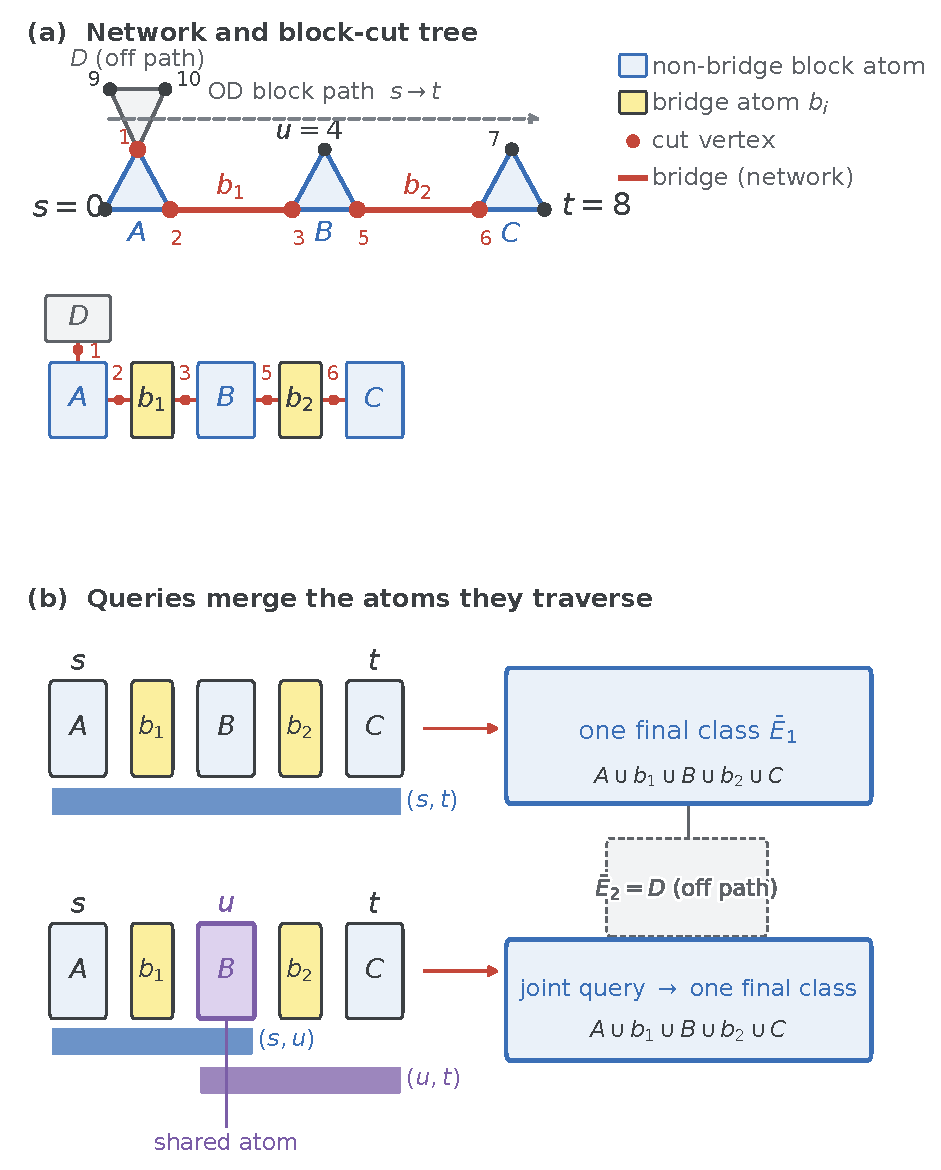
\includegraphics[width=0.74\linewidth]{../figures/fig1_block_cut_v108.pdf}
\caption{(a)~A two-bridge network with its block-cut tree: non-bridge
block atoms $A,B,C,D$ and bridge atoms $b_1,b_2$ joined at shared cut
vertices; the queried OD path runs $s\to t$ and the pendant atom $D$
hangs off the path. (b)~OD queries merge the atoms they traverse: the
single query $(s,t)$ merges $A\cup b_1\cup B\cup b_2\cup C$ into one
class while $D$ stays separate; two queries $(s,u)$ and $(u,t)$ sharing
only atom $B$ merge the same full chain transitively. For the
connected-region comparison of the main text, atom $D$ carries
heterogeneous weights $3,4,5$, invisible to the queried connected
boundaries but violating unrestricted transferability.}\label{fig:blockcut}
\end{figure}

\subsection{Main result: two-sided connected traffic regions}\label{sec:connectedmain}
Traffic analysis typically aggregates on screenlines, cordons and regional
boundaries whose two sides are each spatially connected. The main theorem
shows that this practice buys a substantial freedom in when boundary
summaries transfer. Let
\[
\mathcal U^{\mathrm{conn}}_{st}=\{U\subset V:s\in U,\ t\notin U,
\ G[U]\text{ and }G[V\setminus U]\text{ are connected}\},
\]
where connectivity uses the underlying undirected multigraph. These are
separating bonds: both sides of the boundary form connected regions.

\medskip
\noindent\fbox{\parbox{\dimexpr\linewidth-2\fboxsep-2\fboxrule\relax}{%
\textbf{Main implication.} For two-sided connected traffic regions,
transferable OD boundary explanations require uniform marginal weighting
only along the block atoms traversed by the queried OD paths.
Heterogeneity elsewhere in the network is immaterial to this guarantee.}}
\medskip

\begin{theorem}[two-sided connected-region classification]\label{thm:connectedclassification}
For a connected loopless multigraph, $\mu=e_t-e_s$, and
$D=\operatorname{diag}(w)$, the property
\begin{equation}
\exists\alpha\in\R\quad\forall x\text{ with }Bx=\mu\quad
\forall U\in\mathcal U^{\mathrm{conn}}_{st}:
-\mathbf1_U^\top BDx=\alpha
\label{eq:connectedclassification}
\end{equation}
holds if and only if every edge in the atoms of $\mathcal P(s,t)$ has
one common weight $\alpha$. Weights of edges outside those atoms are
arbitrary, even within an off-path block atom.
\end{theorem}
The proof in Appendix~\ref{app:connectedproof} uses connected prefix and
suffix regions within each traversed atom. Each admissible boundary
crosses edges in just one such atom, which explains why off-path
heterogeneity is invisible to this region family. This is a universal
fixed-weight statement; agreement for one realized response need not
imply its conditions.

\begin{corollary}[several queries on connected regions]\label{cor:connectedmulti}
At one shared weight vector, Eq.~\eqref{eq:connectedclassification} holds
for all queried ODs if and only if edges in each group of atoms joined
by the queried block paths have one common weight. An atom on no queried
path has no weight restriction, including no within-atom restriction.
\end{corollary}
Thus restricting attention to connected traffic regions permits additional
outcome heterogeneity. It changes the compatibility classification,
while the unrestricted extrema and error formulas of
Section~\ref{sec:stability} retain their own stated boundary family.

\subsection{Design implications}\label{sec:design}
The theorem gives three design freedoms, each checkable before any model
is fitted.
\paragraph{Query design.}
Only the atoms traversed by the queried OD paths enter the condition, and
adding queries merges atoms transitively through shared blocks. On
Figure~\ref{fig:blockcut} ($s=0$, $u=4$, $t=8$, linear outcome
$T_w(F)=w^\top F$), the query $(s,u)$ joins $A,b_1,B$ while $b_2$, $C$
and $D$ keep their own constants; adding $(u,t)$ joins the remaining
chain through the shared atom $B$; adjusting only $b_2$ and $C$ then
restores a common account for both queries while the unrelated atom $D$
keeps weight $3$. Appendix~\ref{app:classificationproof} tabulates the
three stages with exact account ranges.
\paragraph{A constructive distinction on Figure~\ref{fig:blockcut}.}
Keep weights $1$ on $A,b_1,B$, weights $2$ on $b_2,C$, but set the three
off-path $D$ weights to $3,4,5$. The first query $(s,u)$ admits common
account $1$ on every two-sided connected region for every conservative
response. The second query $(u,t)$ initially has connected accounts
spanning $[1,2]$ and fails that criterion. Changing only $b_2,C$ to
weight $1$ makes both queries compatible on connected regions, while
$D$ remains internally heterogeneous and the unrestricted criterion
still fails. Two weight configurations document this example:
Appendix~\ref{app:classificationproof} reports the set counts,
circulation-basis verification and account ranges of the three stages
for the uniform-pendant variant of Table~\ref{tab:topologyexample}
(the three $D$ weights all equal to $3$), while the heterogeneous
pendant weights $3,4,5$ used here are verified by the model-specific
diagnosis of Table~\ref{tab:levelsdiag}, whose synthetic row uses
exactly this post-merge configuration.

\paragraph{Outcome design.}
\begin{corollary}[linear outcome functionals]\label{cor:linear}
Let $f\in C^1$ be exactly conservative on an open neighborhood of the
attribution path, and let $T(F)=a^\top F$ be a linear functional of
realized flows. Then $\nabla T\equiv a$, so structural cut consistency
over the unrestricted separating family holds if and only if $a$ is
constant on the compatibility classes, with common cut account
$\beta_j=\Delta q_j\,a|_{\bigcup\mathcal{P}_j}$; over two-sided
connected regions the weaker condition of
Theorem~\ref{thm:connectedclassification} applies instead --- $a$
constant on the block atoms traversed by the queried OD paths, with no
constraint on off-path atoms. Both are conditions on the outcome
definition alone, checkable by inspection before any model is trained,
and the pointwise classification holds at every $\lambda$.
\end{corollary}
Nonlinear compatible outcomes also exist: if
$T(F)=\Phi(\sum_{e\in\bar E_1}F_e,\ldots,\sum_{e\in\bar E_{K'}}F_e)$,
its gradient is class-constant at every flow. More familiar traffic outcomes
require equality of their actual marginal weights. The Beckmann potential
has weights $t_e(F_e)$; total system travel time (TSTT) has weights
$t_e(F_e)+F_et'_e(F_e)$; a separable index $\sum_e g_e(F_e)$ has
weights $g'_e(F_e)$. Heterogeneous link parameters and congestion typically
violate these equalities. A single-link outcome has a nonzero common boundary value
only when the queried OD block path is precisely that singleton bridge.
\paragraph{Region-family design.}
The admissible family is part of the accounting question, and the theorem
quantifies what each choice costs: the connected family ignores off-path
heterogeneity, the unrestricted family does not, and a prescribed finite
family such as a screenline set admits the exact universal test of
Proposition~\ref{prop:familycriterion} in place of a graph-topological
classification.
On public road networks the size of that freedom is itself measurable
from topology alone. Across every positive-demand OD pair, the share of
edges in the queried block atoms --- the share the connected condition
constrains, against $100\%$ for the unrestricted condition --- has
median $100\%$ on Sioux Falls (one atom), $95.4\%$ on Anaheim ($22$
atoms), $95.3\%$ on Winnipeg ($68$ atoms) and $89.1\%$ on
Eastern-Massachusetts ($13$ atoms), where OD pairs localized in a
peripheral block constrain as little as $0.8\%$ of edges. Real urban
cores form large biconnected core blocks, so the off-path release is
modest for a median query and largest for corridor-type or
articulation-adjacent structure; where the release is small, the
realized summaries of Section~\ref{sec:stability}, not the structural
classification, carry the reporting.

\subsection{A stronger criterion for all separating sets}\label{sec:allsets}
When every separating set --- regular or irregular --- must share one
account, the condition tightens and reaches beyond the queried paths.

\Needspace{15\baselineskip}
\begin{theorem}[single-OD classification, static form]\label{thm:t3cpmain}
Let $\mathcal{G}$ be a connected multigraph with one OD pair $(s,t)$,
\textbf{$s\neq t$}, let
$w\in\R^m$, and let $D=\operatorname{diag}(w)$. The
\emph{response-independent OD cut consistency property}
\begin{equation}
\exists\,\alpha\in\R:\qquad BDx=\alpha\,\mu
\quad\text{for every }x\in\R^m\text{ with }Bx=\mu,
\label{eq:t3prop}
\end{equation}
with the scale $\alpha$ independent of the response $x$, holds
\textbf{if and only if}
\begin{enumerate}[(i)]
\item $w$ is constant within every non-bridge atom; and
\item all atoms on the $s$--$t$ block path $\mathcal{P}(s,t)$ share
one common value.
\end{enumerate}
In that case every conservative response induces the same boundary vector:
$BDx=w^*\mu$ for every $x$ with $Bx=\mu$, where
$w^*:=w|_{\bigcup\mathcal{P}(s,t)}$ is the common value of (ii) and
$\alpha=w^*$ is the scale in \eqref{eq:t3prop}.
\end{theorem}

Condition (i) concerns every atom, including those off the OD path. Their
constants may differ; only the traversed atoms must share the scale $w^*$.
Off-path atoms are constrained because a signed circulation can
be added to any conservative response, and heterogeneous weights can turn
it into node divergence. Connected regions change this conclusion, as
Theorem~\ref{thm:connectedclassification} shows. The proof adds a virtual
edge from $t$ back to $s$
(Appendix~\ref{app:classificationproof}): conservative OD responses then
become circulations on the extended graph, so the boundary vector is
response-independent exactly when diagonal weighting preserves the
circulation space --- equivalently, when every weighted cycle has zero
node divergence --- which forces equal weights within each block atom
and one shared weight along the atoms the OD block path connects.

\begin{theorem}[multi-OD classification, static form at a shared
realized flow state]\label{thm:t3cm}
Let $\mathcal{G}$ be connected, let each OD pair satisfy $s_j\ne t_j$,
and let $w\in\R^m$, $D=\operatorname{diag}(w)$. The
response-independent OD cut consistency property \eqref{eq:t3prop}
--- for each queried $j$, some $\alpha_j\in\R$ with
$BDx=\alpha_j\mu_j$ for every $x$ with $Bx=\mu_j$ --- holds
simultaneously for the queried ODs \textbf{if and only if} $w$ is
constant on each OD-compatibility class $\bar{E}_k$.
\end{theorem}

The classification concerns all signed responses compatible with vehicle
conservation; an equilibrium model generally realizes only a subset of
these responses (Appendix~\ref{app:membership}).
All queries use the same realized weight vector. Queries with $\Delta q_j=0$
have zero attribution columns and need not enter the closure. Requiring all
ordered pairs of distinct vertices collapses the classes to one per
connected component (Corollary~\ref{cor:allod}).

\subsection{Pathwise attribution and implications for learned assignment}\label{sec:pathwise}
\begin{corollary}[path form: endpoint implication]\label{cor:path}
Let $f\in C^1$ be conservative on an open set, $T\in C^1$,
$\gamma(\lambda)=q^0+\lambda\Delta q$ the straight-line path with $\Delta q\ne0$, and
$w(\lambda)=\nabla T(f(\gamma(\lambda)))$, $D_\lambda=\operatorname{diag}(w(\lambda))$, shared by
all participating ODs. If the equivalent conditions of
Theorems~\ref{thm:t3cpmain} and~\ref{thm:t3cm} hold at $w(\lambda)$ for
every $\lambda\in[0,1]$, then, for every participating $j$
simultaneously,
\[
B\widetilde{C}_{:,j}=\beta_j\,\mu_j
\]
holds with
\[
\beta_j=\Delta q_j\int_0^1 w^*_{k(j)}(\lambda)\,d\lambda,
\]
where $w^*_{k(j)}$
is the common value on the compatibility class $k(j)$ containing the
atoms of $\mathcal{P}_j$.
\end{corollary}

The specified edgewise outcome and the network representation are both
part of the object. On two series links, an outcome whose marginal
weights oscillate around unity can integrate to the same balanced column
$(1,1)$ as the linear outcome on one demand segment, yet fail to balance
on another (Example~\ref{ex:cancellation}); subdividing a link leaves
the composite map unchanged but creates interior divergence and even
halves the original cut value at the balanced split
(Example~\ref{ex:subdivision}). Response independence concerns
conservative responses on a fixed network; it does not make the account
invariant to road subdivision.

\begin{corollary}[conservative learned assignment]\label{cor:learned}
Let $f^L$ be an exactly conservative learned assignment map on an open
domain. Then its flow-valued integrated gradients inherit OD
conservation, $BG^L_{:,j}=\mu_j\Delta q_j$. Write
$w(\lambda)=\nabla T(f^L(\gamma(\lambda)))$ along the attribution path.
For each $\lambda$, structural cut consistency of the learned
explanations is equivalent to the weight conditions of
Theorems~\ref{thm:t3cpmain} and~\ref{thm:t3cm} at $w(\lambda)$ for the
unrestricted separating family, and to those of
Theorem~\ref{thm:connectedclassification} for two-sided connected
regions. When the unrestricted-family conditions hold at every
$\lambda$, the integrated explanations are realized cut consistent,
$B\widetilde C^{L}_{:,j}=\beta_j\mu_j$
(Corollary~\ref{cor:path}); when they fail at some $\lambda$, the node
representation of Section~\ref{sec:stability} gives the exact spatial
explanation range of the learned column over the unrestricted family
and its exact maximum boundary disagreement from any reference
assignment, with restricted families scanned through the same node
sums.
\end{corollary}
\begin{proof}
The conservation transfer is Eq.~\eqref{eq:anchorchain} applied to
$f^L$. The pointwise equivalences are the two classification theorems
applied to the fixed weight vector $w(\lambda)$; the integral claim is
Corollary~\ref{cor:path} with
$D_\lambda=\operatorname{diag}(w(\lambda))$; the fallback is
Corollary~\ref{cor:boundaryerror}.
\end{proof}
Conservation of predicted flows is thus the first step of a chain whose
later steps are topological; Section~\ref{sec:pairresults} evaluates the
whole chain empirically.

\section{Error-controlled boundary summaries and spatial profiles}\label{sec:stability}\label{sec:algorithm}
\subsection{Obtaining attribution columns}
For a separable outcome $T(F)=\sum_e g_e(F_e)$, a single changing OD gives
\begin{equation}
\widetilde C_{e,j}=g_e(F_e^1)-g_e(F_e^0).
\label{eq:edgeidentity}
\end{equation}
Along this demand path, $dF_e/d\lambda=\Delta q_j\partial_jf_e$; the fundamental theorem of calculus applies link by link, including endogenous background rerouting. Two endpoint assignments therefore recover the attribution column without sensitivity integration. The boundary account is $H_U(F^1)-H_U(F^0)$.
For jointly changing ODs, endpoint differences determine only the sum of attribution columns. Sensitivity integration in Eq.~\eqref{eq:Cdef} separates the individual OD contributions. Both cases then use the same node representation and spatial aggregation (Procedure~\ref{alg:spatial}) below. After preprocessing, all accounts for a prescribed screenline family are obtained from one incidence multiplication and a linear scan; numerical comparisons with direct crossing sums agree to machine precision, and same-task timings against endpoint and vectorized alternatives are collected in Appendix~\ref{supp:timing}.
\subsection{Node representation and exact account ranges}
Once the classes are constructed, structural cut consistency over the
unrestricted family of all separating regions is tested by
\begin{equation}
\eta_{\mathrm{all}}(\lambda)=\max_k\max_{e\in\bar E_k}|w_e(\lambda)-\bar w_k(\lambda)|,
\qquad
\bar w_k=|\bar E_k|^{-1}\sum_{e\in\bar E_k}w_e,
\label{eq:etaall}
\end{equation}
and the joint condition of Theorem~\ref{thm:t3cm} is exactly
$\eta_{\mathrm{all}}=0$. For two-sided connected regions, let
$E_Q=\bigcup_j\bigcup_{A\in\mathcal P_j}A$ collect the edges of all queried
block paths and define
\begin{equation}
\eta_{\mathrm{conn}}(\lambda)=
\max_{k:\,\bar E_k\cap E_Q\neq\varnothing}\;
\max_{e\in\bar E_k}|w_e(\lambda)-\bar w_k(\lambda)|,
\label{eq:etaconn}
\end{equation}
which omits every class on no queried path. By
Corollary~\ref{cor:connectedmulti}, $\eta_{\mathrm{conn}}=0$ is exactly the
connected-region compatibility condition, and off-path atoms may remain
internally heterogeneous, so $\eta_{\mathrm{conn}}=0$ does not imply
$\eta_{\mathrm{all}}=0$. Class construction uses the
block-cut tree and transitive merging; testing a weight vector then needs
one edge scan. No fitted-model derivatives are required for a linear outcome.

For a realized integrated attribution, define
\begin{equation}
d_j=(I-P_{\mu_j})B\widetilde C_{:,j},\qquad
P_{\mu_j}=\frac{\mu_j\mu_j^\top}{\norm{\mu_j}_2^2}.
\label{eq:endpointd}
\end{equation}
Endpoint cut consistency over all separating regions holds precisely when
$d_j=0$; only then does
$\mu_j^\top B\widetilde C_{:,j}/\norm{\mu_j}_2^2$ represent a common cut
value, whatever mechanism produced the balance
(Section~\ref{sec:levels}). For a connected family or another prescribed
finite family, $d_j=0$ is sufficient but not necessary; realized
consistency is then read from the account range over that family.

Without a connectivity restriction, each interior node can enter the
separating set independently. Therefore Eq.~\eqref{eq:cutdiff} gives
\begin{equation}
S_j:=\max_U\phi_j(U)-\min_U\phi_j(U)
=\sum_{v\notin\{s_j,t_j\}}|(B\widetilde C_{:,j})_v|.
\label{eq:cutspread}
\end{equation}
The extrema themselves have a closed form: writing $b_j=B\widetilde
C_{:,j}$, $(x)_+=\max(x,0)$, and summing over interior nodes
$v\notin\{s_j,t_j\}$,
\begin{equation}
\phi_j^{\min}=\phi_j(\{s_j\})-\sum_v(b_{jv})_+,
\qquad
\phi_j^{\max}=\phi_j(\{s_j\})+\sum_v(-b_{jv})_+,
\label{eq:cutextrema}
\end{equation}
since the minimizing set retains exactly the interior nodes with
positive divergence. Subtracting gives, for every separating set $U$
with $I_j=V\setminus\{s_j,t_j\}$,
\begin{equation}
\phi_j(U)-\phi_j^{\min}
=\sum_{v\in I_j\setminus U}(b_{jv})_+
+\sum_{v\in I_j\cap U}(-b_{jv})_+,
\label{eq:cutgap}
\end{equation}
so the gap to the unrestricted minimum is exactly the positive
divergence the region omits plus the negative divergence it contains.
When $\phi_j(\{s_j\})>0$, the unrestricted family
therefore contains a negative account whenever the interior positive
divergence $\sum_v(b_{jv})_+$ exceeds the origin-cut account: node
imbalance, extremal location, and sign crossing are the same statement.
$S_j=0$ is equivalent to $d_j=0$.
The projector in Eq.~\eqref{eq:endpointd} changes only the two endpoint
entries. Cauchy--Schwarz on the $n-2$ interior entries therefore gives
\begin{equation}
S_j=\sum_{v\notin\{s_j,t_j\}}|(d_j)_v|
\le\sqrt{n-2}\,\norm{d_j}_2.
\label{eq:rangebound}
\end{equation}
For network regions whose induced subgraphs and complements are both
connected, define $S_j^{\mathrm{conn}}$ by restricting the same extrema to
that family. Then $S_j^{\mathrm{conn}}\le S_j$. We report both
ranges as percentages of the absolute origin-cut value
$|\phi_j(\{s_j\})|$, which remains explicit because the ratio depends
on that denominator (absolute ranges when it is zero). Within each
region family, the tests of Table~\ref{tab:threequestions} apply with
their family-specific form: the unrestricted column uses
$\eta_{\mathrm{all}}$ and $d_j$, connected families use
$\eta_{\mathrm{conn}}$ and the family's account range, and a
prescribed finite family $\mathcal F$ uses the exact criterion of
Proposition~\ref{prop:familycriterion}; for
maximum model difference, $\mathcal K_j(e_j)$ is exact and family
scans give the restricted value.

\begin{corollary}[best common boundary value]\label{cor:approxinterchange}
For the unrestricted family, the unique best constant in maximum absolute
account error is
\[
\beta_j^\star=\frac{\phi_j^{\max}+\phi_j^{\min}}2
=\frac{(b_j)_{t_j}-(b_j)_{s_j}}2,\qquad
\min_{\beta\in\mathbb R}\max_{U\in\mathcal U_j^{\mathrm{all}}}
|\phi_j(U)-\beta|=\frac{S_j}{2}.
\]
Hence all separating accounts lie within a prescribed absolute tolerance
$\varepsilon$ of some common value if and only if $S_j\le2\varepsilon$.
\end{corollary}
\begin{proof}
For any constant, its largest error at the two attained extrema is at least
half their difference; their midpoint attains this bound for every account.
Equation~\eqref{eq:cutextrema} and $\mathbf1^\top b_j=0$ give the midpoint formula.
\end{proof}
The coefficient agrees with the endpoint projection in
Eq.~\eqref{eq:endpointd}. It approximates the original accounts; it does
not change their edge attribution or define a new system contribution.

\subsection{Common values and minimum-segment summaries}\label{sec:segments}
For any nonempty prescribed finite family $\mathcal F$, the same midpoint argument gives
\begin{equation}
\beta_j^{\mathcal F}=\frac{\phi_{j,\max}^{\mathcal F}+\phi_{j,\min}^{\mathcal F}}2,
\qquad \varepsilon_j^{\mathcal F}=\frac{\phi_{j,\max}^{\mathcal F}-\phi_{j,\min}^{\mathcal F}}2,
\qquad |\phi_j(U)-\beta_j^{\mathcal F}|\le\varepsilon_j^{\mathcal F}\quad(U\in\mathcal F).
\label{eq:familycommon}
\end{equation}
Ordered families --- a corridor's nested screenlines, or the regions of
one projection direction --- additionally support piecewise common
summaries. The construction is stated for any ordered family.
\begin{proposition}[minimal contiguous boundary summary]\label{prop:segmented}
Fix an ordered family of boundary accounts $a_1,\ldots,a_N$ and a
tolerance $\epsilon>0$. Among partitions into contiguous intervals
whose every interval has range at most $2\epsilon$ and does not
strictly mix signs, the longest-feasible-prefix procedure returns one
with the minimum number of intervals. The rule is elementary and
applies to any ordered sequence; its value here is the coupling to the
boundary scan, the node-difference interpretation, and a stated
tolerance --- a single interval reproduces the common summary of
Eq.~\eqref{eq:familycommon}.
\end{proposition}
\begin{proof}
No feasible first interval can extend past the longest feasible prefix,
so every optimal partition starts with a prefix no longer than the
greedy choice; replacing the first interval of an optimal partition by
the full greedy prefix cannot make the remainder infeasible, and the
same argument applies inductively to the remainder.
\end{proof}
The tolerance is the family-scale absolute rule
$\epsilon_j=5\%\max_U|\phi_j(U)|$; a mixed absolute--relative rule
$|\hat a_i-a_i|\le\epsilon_{\mathrm{abs}}+\tau|a_i|$ preserves
relative control at small magnitudes, its feasibility test is inherited
by subintervals so the same greedy returns the minimum count, and
Appendix~\ref{supp:tolerance} reports the sensitivity.
Every query therefore receives a usable output. The reporting rule is
stated once and organizes the numerical sections:

\medskip
\noindent\fbox{\parbox{\dimexpr\linewidth-2\fboxsep-2\fboxrule\relax}{%
\textbf{Adaptive reporting rule.} For a specified boundary family and
relative tolerance $\tau$, report the minimax common value
$\beta_j^{\mathcal F}$ when its exact error satisfies
$\varepsilon_j^{\mathcal F}\le\tau\max(|\phi_{j,\min}^{\mathcal F}|,
|\phi_{j,\max}^{\mathcal F}|)$; otherwise report the boundary response
profile itself, or its minimum contiguous segmentation under the same
tolerance (Proposition~\ref{prop:segmented}).}}
\medskip

\noindent The absolute pair remains available regardless of the
normalization, and each ordered boundary family is summarized at the
coarsest resolution that meets the prescribed tolerance: the outcome is
either an error-controlled common value or an error-controlled
profile.

\subsection{Exact scanning of predefined straight screenlines}\label{sec:scan}
Fix $D$ directions before evaluating attribution. For each direction, sort nodes by their coordinate projection and group equal projection values; no screenline splits such a group. A candidate position is a gap between adjacent groups. Forward and reverse union--find sweeps record whether each prefix and suffix induces a connected subgraph. This geometry and topology preprocessing is reusable across queries, demand paths and models.
For one attribution column, form $b_j=B\widetilde C_{:,j}$ and prefix sums $P_{j,k}=\sum_{i\leq k}(b_j)_{\pi(i)}$. If $s_j$ lies in the prefix and $t_j$ outside, its account is $-P_{j,k}$; for the reverse orientation it is $P_{j,k}$ because $\mathbf1^\top b_j=0$. Retain only endpoint-separating gaps with both sides connected. Scanning these values gives exact accounts and extrema over this prescribed finite screenline family. Preprocessing takes $O(D(|V|\log|V|+|E|\alpha(|V|)))$; after preprocessing, a column takes $O(|E|+D|V|)$ using sparse incidence multiplication. Duplicate regions may be removed without changing extrema.

On Sioux Falls, 36 directions at five-degree intervals give 1642 admissible query--position accounts across six queries (duplicates across directions retained for all algorithms). On exactly these oriented regions, the prefix scan, a vectorized baseline that precomputes the signed crossing matrix $A_{\mathcal F}$ (one sparse row per oriented region, $+1$ leaving and $-1$ entering) and aggregates every account with one sparse product $A_{\mathcal F}C$, and direct crossing-edge summation all agree to $2.2\times10^{-11}$ TSTT units once the reference columns are available. Appendix~\ref{supp:timing} reports the same-task timings of the three aggregations and the amortization threshold of the precomputed matrix.


\subsection{Exact boundary error and response supervision}\label{sec:boundarylearning}
For a query $j$ and any edge vector $h$, define the seminorm
\begin{equation}
\mathcal K_j(h)=\frac12\left(\left|(Bh)_{t_j}-(Bh)_{s_j}\right|
+\sum_{v\notin\{s_j,t_j\}}|(Bh)_v|\right).
\label{eq:boundaryseminorm}
\end{equation}
\begin{corollary}[exact maximum boundary error]\label{cor:boundaryerror}
Let $e_j=\widetilde C^L_{:,j}-\widetilde C^S_{:,j}$ be the difference
between learned and reference attribution columns. Then
\begin{equation}
\max_{U:s_j\in U,\ t_j\notin U}|\phi_j^L(U)-\phi_j^S(U)|
=\mathcal K_j(e_j).\label{eq:exactboundaryerror}
\end{equation}
At a common demand $q$, write
$h_j(q)=D^L(q)J_j^L(q)-D^S(q)J_j^S(q)$.
For any subfamily $\mathcal U_j$ of separating boundaries,
\begin{equation}
\epsilon_j^{\mathcal U}:=\max_{U\in\mathcal U_j}|\phi_j^L(U)-\phi_j^S(U)|
\le |\Delta q_j|\int_0^1\mathcal K_j(h_j(\gamma(\lambda)))\,d\lambda.
\label{eq:localboundarybound}
\end{equation}
\end{corollary}
The proof in Appendix~\ref{app:boundaryerror} applies
Eq.~\eqref{eq:cutextrema} to the error column. Evaluation requires one
incidence multiplication and node scan, without enumerating boundaries.
Connected regions and straight screenlines inherit an upper bound; their
restricted maxima need not equal $\mathcal K_j(e_j)$. The endpoint term
must be retained: the two explanations may each be cut-consistent but
have different common boundary values, which internal imbalance alone misses.

The seminorm evaluates spatial explanation errors directly.
Equation~\eqref{eq:localboundarybound} identifies the weighted response
discrepancy $h_j(q)=D^L(q)J_j^L(q)-D^S(q)J_j^S(q)$ as the direct local
driver of boundary error, and $\mathcal K_j$ defines the corresponding
reference-matching losses, whose complete specifications are collected
in Appendix~\ref{app:learning-objectives}. In the studied assignment
setting the weight-shift component of $h_j$ is small relative to the
response component (Section~\ref{sec:pairresults}), so the unweighted
Jacobian loss is evaluated as a stable proxy for the weighted quantity;
Section~\ref{sec:pairresults} also evaluates the bound chain of
Eq.~\eqref{eq:localboundarybound} directly on the test paths.

\subsection{Total error budget of learned summaries}\label{sec:totalbudget}
Sections~\ref{sec:segments} and~\ref{sec:boundarylearning} control two
errors separately: how far a summary is from the profile it compresses,
and how far a learned profile is from its reference. A reader of a
learned model's explanation uses both at once --- the minimum-segment
summary of the learned accounts. Write $a_j^L(U)$ and $a_j^S(U)$ for
the learned and reference accounts on a family $\mathcal F$,
$\hat a_j^L$ for the learned summary constructed at tolerance
$\varepsilon^{\mathrm{sum}}_j$, and
$\delta_j=\max_{U\in\mathcal F}|a_j^L(U)-a_j^S(U)|$.
\begin{corollary}[total explanation error]\label{cor:totalbudget}
\begin{equation}
\max_{U\in\mathcal F}\bigl|\hat a_j^L(U)-a_j^S(U)\bigr|
\le\varepsilon^{\mathrm{sum}}_j+\delta_j,
\qquad
\delta_j\le\mathcal K_j(e_j)\le|\Delta q_j|\int_0^1\mathcal K_j(h_j(\gamma(\lambda)))\,d\lambda.
\label{eq:totalbudget}
\end{equation}
\end{corollary}
\begin{proof}
Triangle inequality for the split
$\hat a_j^L-a_j^S=(\hat a_j^L-a_j^L)+(a_j^L-a_j^S)$; the first term is
bounded by construction ($\le\varepsilon^{\mathrm{sum}}_j$), the second by
Eq.~\eqref{eq:exactboundaryerror} and Eq.~\eqref{eq:localboundarybound}.
\end{proof}
The budget combines the two outputs the framework delivers --- a
compression and a learned profile --- into the error of the final
artifact. It is a posteriori: the integral bound consumes
reference-response information, so Eq.~\eqref{eq:totalbudget}
characterizes the worst boundary error when reference derivatives are
available, not a deployable guarantee computable from the learned model
alone. Section~\ref{sec:pairresults} evaluates all three quantities on
the test paths.

\begin{algo}[t]
\caption{From an OD demand change to a delivered spatial explanation}\label{alg:spatial}
\small
\textbf{Input:} incidence $B$, query $(s_j,t_j)$, edge attribution $c_j$,
an ordered boundary family $\mathcal F$ with tolerance $\epsilon_j$,
selected regions $U,W$, and optionally a reference column $c'_j$.\\
0. For a single changing OD and separable outcome, obtain $c_j$ from the two endpoint states using Eq.~\eqref{eq:edgeidentity}; for joint changes, input the separately integrated column.\\
1. Compute $b_j=Bc_j$; return its node distribution.\\
2. Return $\phi_j(U)=-\mathbf1_U^\top b_j$ and
$\phi_j(U)-\phi_j(W)=-(\mathbf1_U-\mathbf1_W)^\top b_j$: the boundary
response profile over $\mathcal F$.\\
3. Scan interior nodes to return the extrema in Eq.~\eqref{eq:cutextrema}
and the midpoint and half-range in Eq.~\eqref{eq:familycommon},
and their sets $\{s_j\}\cup\{v\in V\setminus\{s_j,t_j\}:b_{jv}>0\}$ and
$\{s_j\}\cup\{v\in V\setminus\{s_j,t_j\}:b_{jv}<0\}$.\\
4. Summarize: if $\varepsilon_j^{\mathcal F}\le\epsilon_j$ return the common
value $\beta_j^{\mathcal F}$; otherwise apply
Proposition~\ref{prop:segmented} and return the minimum-segment
summary with each segment's position range, representative value and
worst error ($\le\epsilon_j$ by construction).\\
5. If $c'_j$ is supplied, return $\mathcal K_j(c_j-c'_j)$ as the exact
maximum absolute error over unrestricted separating regions, the family
scan over $\mathcal F$, and, when step 4 produced a summary, the total
budget $\varepsilon^{\mathrm{sum}}_j+\delta_j$ of
Eq.~\eqref{eq:totalbudget}.\\
The incidence product and scan cost $O(|E|+|V|)$ per column; selected-region
sums cost $O(|V|)$; the segmentation is one linear pass over the family.
The same node representation serves all these tasks. The columns must already
have been computed; their reference-attribution cost remains separate.
\end{algo}



\paragraph{Scope and interpretation.}\label{sec:noninheritance}
The classification fixes four objects before any model is fitted: the
road representation (subdivision changes which crossing-link costs a
boundary includes, Example~\ref{ex:subdivision}); the outcome
definition (its marginal weights are the classified object); the
attribution path in demand space (with several ODs changing jointly,
the per-query columns are path dependent; the total is not); and the
admissible region family. The structural, model-specific, realized and
learned-reference levels answer different questions and are reported
separately (Table~\ref{tab:threequestions}).

\paragraph{Approximate conservation.}
For a model with residual $r(q)=Bf(q)-Mq-b$ and constant $b$, the
corresponding flow-attribution residual is
\begin{equation}
R_j:=BG_{:,j}-\mu_j\Delta q_j
=\Delta q_j\int_0^1\partial_jr(\gamma(\lambda))\,d\lambda,
\qquad \sum_jR_j=r(q^1)-r(q^0).
\label{eq:residualidentity}
\end{equation}
Small endpoint residuals control the sum, but individual columns can cancel.
Approximate output conservation controls attribution residuals only when
derivative regularity is also available; Appendix~\ref{app:approx} gives
the $C^{1,1}$ conditions, a local bound, sharpness examples and an
extension to weighted accounts. The traffic experiments below use exactly
conservative models.

\section{Numerical evidence and transportation interpretation}\label{sec:numerics}
Sioux Falls absolute accounts use benchmark flows in veh/h and time units of $0.01$ h; multiply an account by $0.01$ for the hourly vehicle-hour total. Anaheim uses vehicle-minutes per hour. All experiments use the stated fixed-path logit-SUE assignment models and prespecified demand scenarios; shares reported over boundary families are enumeration shares over those families. The adaptive reporting rule of Section~\ref{sec:stability} organizes the experiments: every query either receives one error-controlled common value or an explicit spatial profile. The subsections examine, in order, how that selection varies across demand and congestion regimes, which traffic mechanisms generate the spatial variation and how stable they are under alternative attribution paths, and what complete profiles with compact summaries look like on a large network.

\subsection{Adaptive summary selection across demand and congestion regimes}\label{sec:adequate}
Sioux Falls has 24 nodes and 76 arcs in one block atom. Its structural weight condition is therefore the same for every OD, and the connected and unrestricted classifications coincide; the experiments measure variation due to realized responses and heterogeneous marginal costs. The query-dependent classification is illustrated separately in Figure~\ref{fig:blockcut}.

Six input-selected queries away from node 10 change jointly from $0.2$ to $1.6$ times their base values with all other demands fixed and routes responsive; they are the shortest and longest free-flow ODs in each demand tercile (Appendix~\ref{supp:newod}). Table~\ref{tab:newod} reports their ranges. The adaptive rule separates them sharply: the geometric accounts for $(7,18)$ lie in $[642,702]$, their midpoint $672$ has maximum absolute error $30$, or $4.3\%$ of the largest account, and this family admits one common summary at a $5\%$ tolerance; the $(1,19)$ and $(7,12)$ geometric ranges cross zero and require boundary-specific reporting at every tolerance considered below.
\begin{table}[pos=htbp]
\footnotesize
\caption{System contributions and spatial ranges for six prespecified queries,
setting C (TSTT units). Connected: all admissible connected regions;
screenline: the geometric family constructed independently of attribution
values. All $C_j$ are positive. Origin-cut accounts, negative shares, and
neighbourhood ranges are retained in Appendix~\ref{supp:newodaccuracy}.}
\label{tab:newod}
\small
\begin{tabular*}{\tblwidth}{@{\extracolsep{\fill}}lrrr}
\toprule
OD & $C_j$ & Connected [min, max] & Screenline [min, max]\\
\midrule
$(7,18)$ & $672.9$ & $[634{,}\ 710]$ & $[642{,}\ 702]$ \\
$(1,19)$ & $50{,}097.7$ & $[-13{,}502{,}\ 24{,}260]$ & $[-2{,}767{,}\ 22{,}124]$ \\
$(4,5)$ & $2{,}826.0$ & $[2{,}396{,}\ 3{,}452]$ & $[2{,}652{,}\ 3{,}176]$ \\
$(1,15)$ & $77{,}403.2$ & $[-8{,}286{,}\ 40{,}540]$ & $[511{,}\ 36{,}621]$ \\
$(6,8)$ & $73{,}964.9$ & $[35{,}307{,}\ 66{,}695]$ & $[45{,}230{,}\ 65{,}286]$ \\
$(7,12)$ & $117{,}482.3$ & $[-17{,}616{,}\ 60{,}029]$ & $[-2{,}967{,}\ 57{,}780]$ \\
\bottomrule
\end{tabular*}
\end{table}

Experiment C widens the view to an input-only selection of 18 of the 528 positive Sioux Falls OD demands, taking two lexicographically predetermined positions from each demand-by-free-flow-time tertile cell. Each OD changes alone over $\pm10\%$ and $\pm20\%$ intervals while other demands remain fixed with endogenous rerouting; the same 36-direction geometric family is used throughout, and Appendix~\ref{sec:coverage} reports every query and both widths. For each nonempty family, let $\beta=(\phi_{\max}+\phi_{\min})/2$ and $\varepsilon=(\phi_{\max}-\phi_{\min})/2$. This common summary minimizes the largest absolute discrepancy, so every reported boundary satisfies $|\phi(U)-\beta|\leq\varepsilon$. The reported normalized error is
\begin{equation}
r_j^{\mathcal F}=100\,\varepsilon_j^{\mathcal F}\Big/\max\bigl(|\phi_{j,\min}^{\mathcal F}|,|\phi_{j,\max}^{\mathcal F}|\bigr),
\label{eq:normerror}
\end{equation}
the absolute deviation of every account from the common value as a
percentage of the family's largest account magnitude; it does not bound
each account's own relative error. We apply a fixed descriptive tolerance
$r_j^{\mathcal F}\leq5\%$; this is a reporting choice rather than a
transport welfare threshold. When all accounts in a family share one
sign, $r_j^{\mathcal F}\leq50\%$, so values near $50\%$ indicate that
the smallest magnitude is far below the largest, not that the accounts
nearly agree.
At $\pm10\%$ and $\pm20\%$, respectively, 1 and 1 of 18 queries meet this tolerance, while 1 and 1 have accounts of both signs; representative common summaries at $\pm20\%$ appear in Appendix~\ref{sec:coverage}.

\begin{figure}[t]\centering
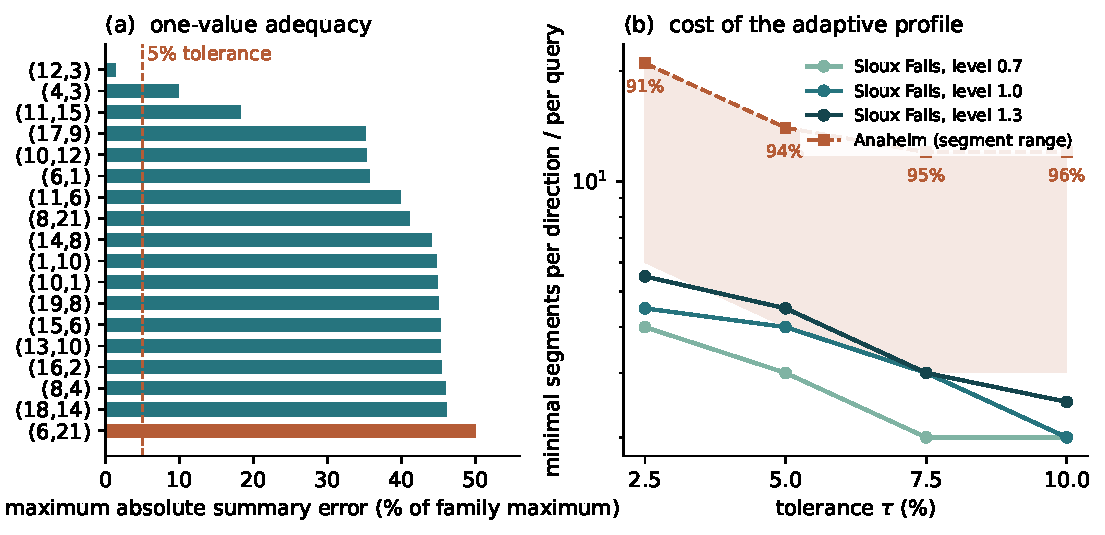
\includegraphics[width=0.99\linewidth]{../figures/fig_v108_summary_frontier.pdf}
\caption{Adaptive summary selection and its cost. Left: maximum absolute
summary error (Eq.~\eqref{eq:normerror}) over all 18 input-stratified
queries at $\pm20\%$, with the queries reordered by error; the $5\%$
tolerance marks which queries receive one common value. Right: the
alternative output --- median minimal segments per projection
direction on Sioux Falls (36 normals, distinct chains deduplicated,
three load levels) and per-query segments on Anaheim's ordered
families --- as the tolerance varies from $2.5\%$ to $10\%$;
underlying numbers in Table~\ref{tab:tolerance}
(Appendix~\ref{sec:coverage}).}\label{fig:commonsummary}\end{figure}

Figure~\ref{fig:commonsummary} presents the selection and its cost. A
minority of queries admits one common value at a working tolerance;
every other query is summarized one direction at a time. On Sioux
Falls the 36 projection normals of the geometric family induce
22--35 distinct ordered chains per query (median 5--9 regions per
chain), and consecutive entries of one chain are nested along that
direction, so the chain --- not the merged sequence --- is the unit of
spatial contiguity. Segmenting each chain at the family tolerance
needs a median of $2$--$5.5$ segments per direction across the three
load levels as the tolerance ranges over $2.5$--$10\%$ (at the $5\%$
tolerance and baseline load: median $4$, maximum $8$), and relaxing
the tolerance to $10\%$ halves the median to $2$. Ordering all
directions into one progress sequence yields fewer apparent segments
only by grouping non-adjacent cross-sections, so those counts are not
spatial summaries and are retained only for comparison
(Table~\ref{tab:tolerance}); the per-direction profiles are what the
framework delivers. On Anaheim's single-direction ordered families
the same relaxation raises the compression of the 83--211 accounts
per query from $91.4\%$ (6--21 segments) to $96.4\%$ (3--12
segments). With the same segment count, equal-count partitions have
median worst-segment error $1.4$--$4.0$ times the greedy error per
direction on Sioux Falls and $4.7$--$18.8$ times the tolerance on
Anaheim, so position-aware segmentation is what buys the error
control, not the segment count alone.

The $\pm10\%$ and $\pm20\%$ summaries of the same 18 queries are close in normalized terms, so further subdividing the perturbation width adds little information. The congestion state of the baseline is the more informative axis. All 528 demands are scaled jointly to $0.7$, $1.0$ and $1.3$ times their published values; at each level the level equilibrium is solved once, the focal query alone moves by $\pm20\%$, other demands stay fixed with responsive routes, and the endpoint identity supplies the attribution column (solver protocol in Appendix~\ref{supp:newod}).
\begin{table}[t]\centering\footnotesize
\caption{Common-summary statistics across baseline load levels (18
queries, focal $\pm20\%$, same 36-direction family). Normalized error
is Eq.~\eqref{eq:normerror}; the ratio column is the median
geometric-to-unrestricted spread ratio.}\label{tab:loadlevels}
\begin{tabular}{rrrrrr}\toprule
Level & Queries within $5\%$ & Mixed signs & Median error (\%) & Median ratio & Max.\ negative share\\\midrule
$0.7$ & 2 & 0 & 34.5 & 0.529 & $0.00\%$\\
$1.0$ & 1 & 1 & 44.4 & 0.574 & $0.67\%$\\
$1.3$ & 0 & 3 & 45.2 & 0.563 & $4.03\%$\\
\bottomrule\end{tabular}\end{table}
Table~\ref{tab:loadlevels} shows a monotone pattern: under the light
baseline, accounts are flatter across the family --- the median
normalized error falls to $34.5\%$, two queries satisfy the $5\%$
tolerance and no family crosses zero --- whereas the heavy baseline
makes every query exceed the tolerance, three families mix signs and
the negative share of $(6,21)$ reaches $4\%$. Per-query normalized
errors rise from the light to the heavy level for 17 of 18 queries
(e.g.\ $(10,12)$: $18.6\to35.2\to40.3$; $(1,10)$: $31.2\to44.8\to48.0$).
Across the load levels, light-load conditions admit transferable single
summaries more often, and heavy-load conditions require
boundary-specific reporting. The load-level trend has a theory-side
counterpart: the node-imbalance norm $\norm{d_j}_2$ rises by a factor
of $13.2$ from the light to the heavy baseline, and Eq.~\eqref{eq:cutspread}
sums that imbalance into the spatial range
(Appendix~\ref{sec:coverage} reports the rank correlations and the
Cauchy--Schwarz comparison).

\paragraph{How much does the model-specific level buy?}\label{sec:levelsdiag}
The universal structural condition quantifies over all conservative
responses; Section~\ref{sec:levels} introduced the model-specific level
that reasons on the responses an assignment model can actually realize.
Table~\ref{tab:levelsdiag} evaluates the hierarchy numerically. On the
Figure-1 network with its published post-merge weights, the universal
condition fails because the off-path pendant atom is heterogeneous, yet
the model-specific tests hold exactly for the all-simple-paths
structure: every rerouting that model can make preserves the common
account, so restricting attention to realizable responses restores
transferability that the universal condition denies. On Sioux Falls the
two levels coincide --- the full-background fixed-path model spans the
complete circulation space through path exchanges, so its response
envelope contains every conservative response
(Appendix~\ref{supp:networks}) --- and both fail at realistic TSTT
weights, leaving the realized summaries of Table~\ref{tab:newod} as the
operative output. The diagnosis is stable across load levels: the
normalized universal violation stays within $2.08$--$2.21$ from the
$0.7$ to the $1.3$ baseline while $\rho_{\mathrm{swap}}$ falls from
$1.12$ to $0.80$ as congestion grows. On Anaheim the universal test
fails more decisively (normalized violation $10.08$) and the
model-specific test fails with it ($\rho_{\mathrm{swap}}=2.18$ over the
$404$-dimensional exchange space), so there too the realized layer
carries the reporting.
\begin{table}[t]\centering\footnotesize
\caption{Numerical diagnosis of the transferability hierarchy of
Table~\ref{tab:threequestions}. $\eta_{\mathrm{all}}$ and
$\eta_{\mathrm{conn}}$: weight spread within all atoms / within the
queried atoms, normalized by the mean weight. $\rho_{\mathrm{swap}}$:
weighted-divergence leakage of unit rerouting directions relative to a
unit reference response; $\rho_{\mathrm{swap}}=0$ certifies
$BDN=0$, and together with zero off-span residuals
$\rho_{\mathrm{ref},j}$ it certifies both conditions of the
model-specific level. On Sioux Falls (level $1.0$) three of the six
queries have $\rho_{\mathrm{ref},j}=0$; the other three lie in
$0.83$--$0.97$. Realized: median
normalized geometric common-summary error of the setting-C six
queries. Synthetic: published post-merge weights; Sioux Falls: TSTT
weights at the level-$1.0$ equilibrium, where the path-exchange space
attains the full circulation dimension $53$.}\label{tab:levelsdiag}
\begin{tabular}{lrrrr}\toprule
Network & $\eta_{\mathrm{all}}$ & $\eta_{\mathrm{conn}}$ & $\rho_{\mathrm{swap}}$ & Realized (\%)\\\midrule
Figure-1 synthetic & $0.61$ & $0$ & $0$ & $0$ (model responses)\\
Sioux Falls & $2.08$ & $=$ & $0.88$ & $32.3$\\
\bottomrule\end{tabular}\end{table}

\subsection{What generates spatial variation?}\label{sec:variation}
Experiment A varies the background treatment. Eight largest published OD demands, all incident to node 10, change jointly from $0.2$ to $1.6$ times their base values; every study OD has ten fixed paths. Settings A, B and C use zero background, frozen background link flows and fixed background demands with endogenous rerouting, respectively. Setting C assigns all 528 positive demands (full protocols in Appendix~\ref{supp:fields}).
Uniform weights provide a compatible control. The active-link outcome $T(F)=F_{10\to16}$ preserves the $(10,16)$ direction but permits a response-dependent scale; TSTT produces internal imbalance. Figure~\ref{fig:respfield} illustrates the three patterns on the same realized response: compatible weights give one common account on every boundary, the directional outcome balances along the OD but scales with the response, and TSTT weights generate genuine spatial structure. For its seed-zero TSTT response, expanding $\{10\}$ to $\{10,17\}$ lowers the account from $5.77\times10^4$ to $4.34\times10^4$, approximately $92\%$ of the unrestricted spread. The direct-SUE decrease is $24.80\%$ of its own origin-cut account (Appendix~\ref{supp:accuracy}). Both sides of these regions are connected. Free-flow weights explain $84.7\%$ of the node-17 imbalance: all incident links have free-flow time 2 except $10\leftrightarrow17$ with time 8, giving $[B\operatorname{diag}(t_0)G_j]_{17}=6(G_{10\to17,j}-G_{17\to10,j})$.
\begin{figure}[pos=t]
\centering
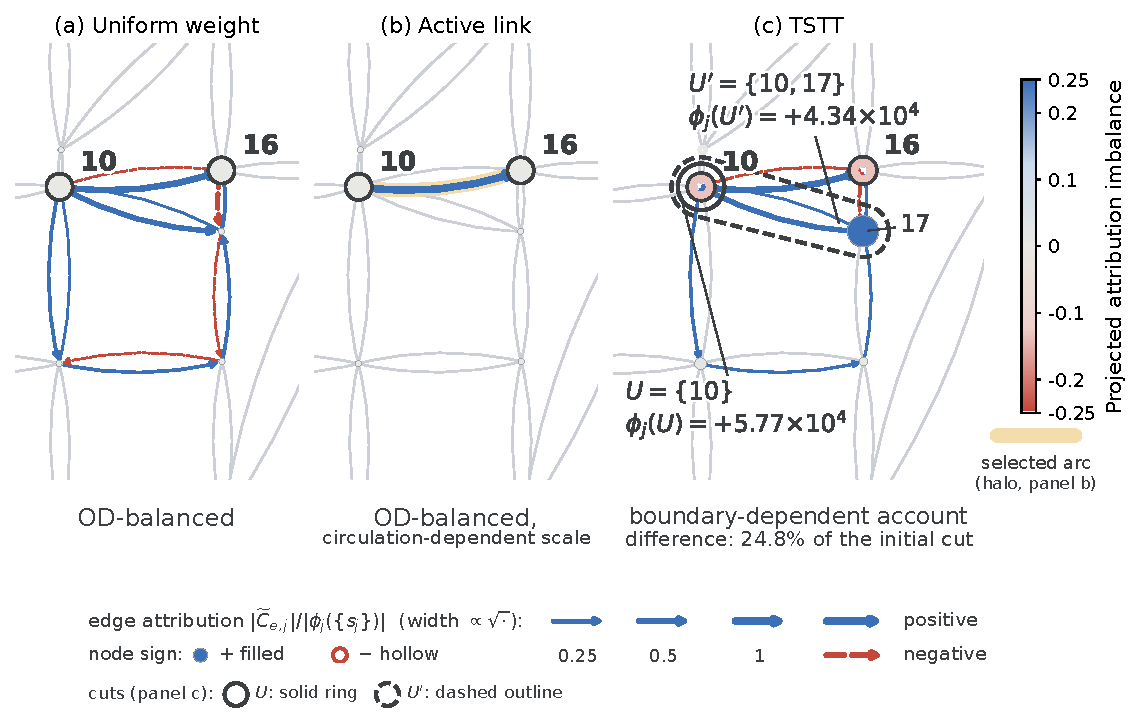
\includegraphics[width=0.9\linewidth]{../figures/fig_resp_field_v100.pdf}
\caption{OD $(10,16)$ endpoint attributions, zero background, learned
seed $0$. (a) Uniform weights give cut consistency. (b) The active-link
outcome balances in the OD direction but has no response-independent
scale. (c) The signed TSTT boundary account decreases by $24.8\%$ when
the boundary expands from $\{10\}$ to $\{10,17\}$. Widths encode
attribution magnitude; node colors show the projected attribution
imbalance $(d_j)_v$ (Eq.~\eqref{eq:endpointd}) divided by the absolute
origin-cut value.}
\label{fig:respfield}
\end{figure}

Table~\ref{tab:cutspreadperod} shows three representative queries of the eight under the three background settings (the complete table is in Appendix~\ref{supp:additional}); rerouting produces appreciable spatial variation for every query, and connected regions retain $60.41$--$76.85\%$ of the unrestricted range across the full set. Normalizations use each setting's own origin account: for $(17,10)$, the percentage falls from $59.95\%$ in A to $54.77\%$ in C while the absolute spread rises from 17,607.8 to 123,202.1, approximately sevenfold.
\begin{table}[pos=htbp]
\footnotesize
\caption{TSTT cut ranges as percentages of each account's absolute
origin-cut value; three representative queries shown, complete table in
Appendix~\ref{supp:additional}. A: zero background; B: frozen background
flows; C: background demands fixed, all traffic re-equilibrated. Learned
values are five-seed medians (ranges); all SUE columns are direct
($41$ quadrature points, implicit sensitivities).}\label{tab:cutspreadperod}
\small
\begin{tabular*}{\tblwidth}{@{\extracolsep{\fill}}lccccc}
\toprule
& \multicolumn{4}{c}{Unrestricted range (\%)} & Connected (\%)\\
\cmidrule(lr){2-5}\cmidrule(lr){6-6}
OD & Learned A & SUE A & SUE B & SUE C & SUE C\\
\midrule
$(17,10)$ & $59.71$ $(58.92$--$61.23)$ & $59.95$ & $56.38$ & $54.77$ & $35.27$ \\
$(16,10)$ & $36.80$ $(36.41$--$38.40)$ & $36.86$ & $39.99$ & $166.26$ & $127.72$ \\
$(11,10)$ & $0.18$ $(0.03$--$0.27)$ & $0.0073$ & $0.79$ & $81.09$ & $48.98$ \\
\bottomrule
\end{tabular*}
\end{table}
\paragraph{Same-state response decomposition.}\label{subsec:bgsplit}
Comparing A, B and C changes both costs and sensitivities. At each common setting-C state, split responses into study and background parts, with $BJ_j^{\mathrm{study}}=\mu_j$ and $BJ_j^{\mathrm{bg}}=0$. Weight both by the same total-flow TSTT gradient, yielding
\begin{equation}
\widetilde C_j^{\mathrm{tot}}=\widetilde C_j^{\mathrm{study}}+\widetilde C_j^{\mathrm{bg}}.
\label{eq:bg_attribution}
\end{equation}
At node 15 for $(10,16)$, study and background divergence contributions are $-973.1$ and $49{,}103.4$. Yet on the specified expansion $\{10\}\to\{10,17\}$, the account changes only $-3361.1$ ($-1305.0$ study, $-2056.1$ background), or $1.23\%$ of the initial account. Large extremal variation can coexist with similar selected accounts. Component differences add at a fixed region pair; their separate ranges do not add in general.

\paragraph{Free-flow and congestion mechanisms.}\label{subsec:newod}
For BPR costs, $g_e'=t_{0,e}+0.75t_{0,e}(F_e/c_e)^4$. Crossing these two weight terms with the two response terms gives four additive contributions, evaluated at identical states and the same reported boundary:
\[
\phi_j(U_-)=\sum_{a\in\{\mathrm{ff,cong}\}}\sum_{b\in\{\mathrm{study,bg}\}}\phi_j^{a,b},
\qquad \phi_j^{a,b}=-\Delta q_j\int_0^1\mathbf1_{U_-}^{\top}BD_\lambda^aJ_j^b(\lambda)\,d\lambda.
\]
Table~\ref{tab:ffcong} distinguishes the mechanisms behind the sign-crossing queries of Table~\ref{tab:newod}: study congestion dominates $(1,19)$, both congestion terms are negative for $(1,15)$, and background congestion dominates $(7,12)$. The combined free-flow contribution stays positive. The decomposition is additive at a common equilibrium state and identifies the contribution of each response--weight component.
\begin{table}[pos=htbp]
\caption{Four parts of the same boundary account at the reported
$U_-$ (setting C, six-query protocol; TSTT units; identical $41$-point
states, responses, and boundaries as Table~\ref{tab:newod}). Study
includes all six query ODs; background includes the other $522$.
Columns cross free-flow/congestion weights with study/background
responses. Entries are rounded independently.}\label{tab:ffcong}
\small
\begin{tabular*}{\tblwidth}{@{\extracolsep{\fill}}lrrrrr}
\toprule
OD & Free-flow study & Free-flow background & Congestion study & Congestion background & Total\\
\midrule
$(1,19)$ & $-361.3$ & $+759.0$ & $-17{,}357.9$ & $+3{,}458.6$ & $-13{,}501.6$ \\
$(1,15)$ & $+1{,}541.8$ & $+333.8$ & $-6{,}537.4$ & $-3{,}624.2$ & $-8{,}286.0$ \\
$(7,12)$ & $+3{,}897.0$ & $-1{,}311.1$ & $+125.5$ & $-20{,}327.6$ & $-17{,}616.2$ \\
\bottomrule
\end{tabular*}
\end{table}
The sign pattern itself is a spatial property, not a magnitude artefact. Negative accounts occupy $17.8\%$, $2.5\%$ and $7.3\%$ of the 14,477, 15,191 and 16,943 connected regions of the three sign-crossing queries. For $(1,19)$, the connected minimum $-13{,}501.6$ is attained on a 13-node region, whereas a 13-node free-flow neighbourhood has account $+10{,}756.0$: region size alone does not determine the account. At the minimizing boundary, outgoing attributions sum to $7{,}867.3$ and incoming attributions to $21{,}368.8$, so the signed crossing-link account is negative while $C_j=50{,}097.7>0$; Figure~\ref{fig:negmech} maps all 26 crossing links. Figure~\ref{fig:screenlines} shows the same contrast on two straight screenlines of the prespecified geometric family: the minimum and maximum screenline accounts of $(1,19)$ have opposite signs under one positive network-wide contribution.
\begin{figure}[pos=tb]
\centering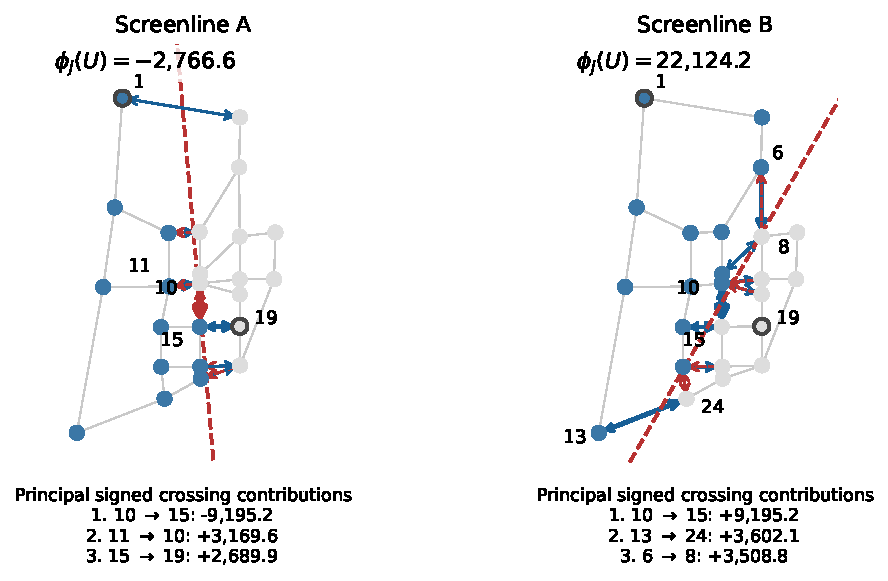
\includegraphics[width=0.64\linewidth]{../figures/fig_screenlines_v108.pdf}
\caption{Contrasting screenline accounts for the same positive OD
contribution. Two straight screenlines for OD $(1,19)$, setting C. Blue
nodes belong to $U$; grey nodes are outside; dashed lines separate the
two sides. Node $1$ is inside and node $19$ outside in both panels.
The two lines have different normal directions, so they are labelled
Screenline~A (left) and Screenline~B (right); the crossing progress of
each with the straight origin--destination segment is $0.61$ and
$0.78$, an ordering of the crossing positions that does not by itself
make the two enclosed regions nested. The two accounts have
opposite signs while the network-wide contribution is positive. The
lines are the minimum and maximum of the prespecified geometric family;
the complete irregular connected minimum and its crossing-link
decomposition appear in Figure~\ref{fig:negmech}.}
\label{fig:screenlines}\end{figure}
The straight-screenline family uses 36 directions at $5^\circ$ intervals, gaps between node projections, two-sided connectivity and duplicate removal; construction is independent of attribution. It contains 23--152 distinct regions per query. The $(1,19)$ and $(7,12)$ negative minima occur on 2/152 and 10/148 screenlines. Origin-centred hop and free-flow neighbourhoods remain positive but can differ in magnitude by factors 8.9, 9.0 and 3.4 for the three sign-crossing queries (Appendix~\ref{supp:newodaccuracy}). Sign stability and common-value accuracy are distinct properties.

\paragraph{Stability under alternative attribution paths.}\label{subsec:pathrobust}
With several ODs changing jointly, the per-query attribution columns
depend on the demand path; the columns are defined here under the
straight-line transition, and this paragraph quantifies that
dependence. Twenty-two piecewise-linear alternatives --- the six study
ODs changing one at a time, in canonical order, reverse order, and
twenty fixed-seed random permutations --- are compared with the
straight line on the setting-C protocol, with identical endpoints,
solver tolerance, quadrature and boundary family, and with the
mechanism decomposition evaluated at the same fixed regions $U_-$; the
total outcome change is path independent and reproduces to
$1.5\times10^{-7}$ relative on every order.
\begin{table}[t]\centering\footnotesize
\caption{Attribution-path robustness on the setting-C six-query
protocol: straight-line joint path versus 22 one-at-a-time orders
(canonical, reverse, 20 seeded permutations). $C_j$ range: minimum and
maximum over the orders; deviation relative to the straight-line
value. $\varepsilon$ shift: median normalized common-summary error
over the orders against the straight-line value. Sign: orders whose
family range keeps the straight-line sign-crossing status; mechanism:
orders whose largest-magnitude component at $U_-$ matches the straight
line's.}\label{tab:pathrobust}
\begin{tabular}{lrrrrr}\toprule
OD & $C_j$ range & Max $|C_j|$ dev. & $\varepsilon$ shift & Sign & Mechanism\\\midrule
$(7,18)$ & $[666.5,\ 678.4]$ & $1.0\%$ & $4.3\%\to4.3\%$ & $22/22$ & ---\\
$(1,19)$ & $[48{,}451.9,\ 51{,}817.7]$ & $3.4\%$ & $56.3\%\to56.4\%$ & $22/22$ & $22/22$\\
$(4,5)$ & $[2{,}780.8,\ 2{,}911.4]$ & $3.0\%$ & $8.2\%\to8.2\%$ & $22/22$ & ---\\
$(1,15)$ & $[75{,}306.6,\ 79{,}553.2]$ & $2.8\%$ & $49.3\%\to49.3\%$ & $22/22$ & $22/22$\\
$(6,8)$ & $[72{,}157.8,\ 75{,}713.7]$ & $2.4\%$ & $15.4\%\to15.5\%$ & $22/22$ & ---\\
$(7,12)$ & $[117{,}367.2,\ 117{,}573.5]$ & $0.1\%$ & $52.6\%\to52.5\%$ & $22/22$ & $22/22$\\
\bottomrule\end{tabular}\end{table}
Table~\ref{tab:pathrobust} summarizes the outcome. The spatial
conclusions are order-insensitive: system contributions move by at most
$3.4\%$, every query's sign-crossing status over the family is
identical on all 22 orders, the normalized common-summary errors shift
by at most $0.2$ percentage points, and the dominant mechanism at $U_-$
is unchanged on every order. The profile deviations themselves are
bounded (medians $0.3\%$--$4.5\%$, maxima $0.3\%$--$4.7\%$ of the
largest straight-line account), so the reported profiles are
path-specific in their fine structure but not in their traffic
interpretation. Per-order detail is retained in
Appendix~\ref{supp:pathrobust}.

\subsection{Complete spatial profiles and compact summaries}\label{sec:anaheim}
The public Anaheim network has 416 nodes, 914 directed links and 1,406 positive OD demands \citep{tnfrc2024transportation}. Six largest demands change jointly from 0.8 to 1.2 times their published values; other demands remain fixed with endogenous route choices. Ten fixed free-flow shortest paths per OD exclude other zone centroids as intermediate nodes (first through node 39). This calculation uses the existing 41-state attribution columns.
To obtain interpretable region locations without requiring coordinates, define free-flow progress $p(v)=[d_s(v)-d_t(v)+d_s(t)]/[2d_s(t)]$, using shortest distances in the underlying undirected network with the smaller free-flow time on parallel roads --- a network-distance indicator used for ordering the family, not a behavioural travel progress (assignment paths additionally exclude other zone centroids, the progress metric does not). The origin has progress zero and destination progress one. Group tied levels, retain prefixes with two connected induced sides that separate the OD, and orient every region toward the origin. This distance-based family depends on the network and query, before inspecting any attribution. It is a prescribed family, not all connected regions, and it is single-direction: the nested prefixes are totally ordered by progress, so no direction grouping is needed here.

The case asks one transport question: how does the signed crossing-cost
response of the demand change evolve along the origin--destination
direction, and does the variation come mainly from the study traffic's
congestion adjustment or from background rerouting?
Figure~\ref{fig:anaheimprofile} gives the answer for the query with the
largest early--late difference: the account as a function of progress
over the complete family with its delivered four-segment summary, and
the four-part same-state decomposition along the same axis. The
profiles of the remaining five queries stay positive with family ranges
spanning roughly one to one and a half orders of magnitude
(largest-to-smallest account ratios 12.5--36.9); the complete per-query
numbers --- system contributions, unrestricted and family ranges,
region counts and the accounts of the three prespecified positions ---
are collected in Appendix~\ref{app:anaheimsettings}
(Table~\ref{tab:anaheim}), with the early--late mechanism differences
in Table~\ref{tab:anaheimmechanism}.
\begin{figure}[t]\centering
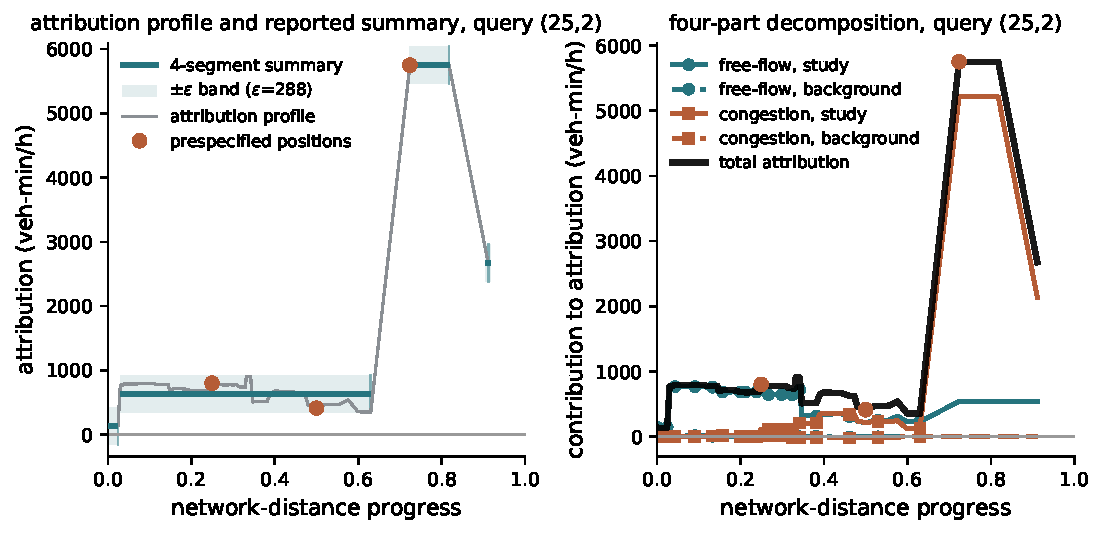
\includegraphics[width=0.99\linewidth]{../figures/fig_v108_anaheim_profile.pdf}
\caption{Anaheim spatial response profile for query $(25,2)$ over the
distance-based family, with its delivered summary. Left: the account
versus free-flow progress along its own OD direction (grey curve); the
four-segment minimum summary at the family tolerance is overlaid
(teal step curve with $\pm\epsilon$ band, $\epsilon=287.6$), and ochre
dots mark the three prespecified positions (nearest admissible gaps to
progress $0.25$, $0.50$, $0.75$). Right: the four-part same-state
decomposition, crossing free-flow and congestion weights with study
and background responses at identical states (teal: free-flow weights,
ochre: congestion weights; solid: study response, dashed: background);
the grey curve is the total account. Components close within
$2\times10^{-12}$ vehicle-minutes per hour.}\label{fig:anaheimprofile}
\end{figure}
Query $(25,2)$ falls from 801.5 at progress $0.250$ to 412.0 at $0.500$
and then rises to the family maximum 5751.2, which holds on the plateau
from progress $0.724$ to $0.818$ before falling back to 2673.1 at
$0.911$. The delivered summary is four segments
(Table~\ref{tab:anaheimsegments}): an origin-side segment near the
family minimum, a long corridor segment covering progress $0.03$--$0.63$
at representative value $630.2$, the congestion plateau at $5751.2$,
and a destination-side position at $2673.1$; every account lies within
$\epsilon=287.6$ of its segment value, the tolerance being $5\%$ of the
family maximum. The decomposition panel locates the mechanism. At the
early position the account is dominated by the free-flow study response
($669.3$ of the total $801.5$, congestion study $111.5$, background
below $11$); at the middle position the two study terms are comparable
($211.5$ free-flow against $212.6$ congestion of the total $412.0$,
background below $11$); at the late position the congestion study term
reaches $5213.7$ while both background terms are below $0.1$ in
absolute value: the rise is congestion adjustment of the study traffic
itself on destination-side links, not background rerouting. The
decomposition is additive at a common equilibrium state and identifies
the contribution of each response--weight component; the summary then
states, with its error bound, where that variation changes.
\begin{table}[t]\centering\footnotesize
\caption{Delivered minimum-segment summaries on Anaheim at the family
tolerance ($5\%$ of the largest account magnitude per query,
Proposition~\ref{prop:segmented}). Segment values are midpoints of the
enclosed account range; every account in a segment lies within the
query's $\epsilon$ of the stated value. Detail for the remaining
queries appears in Appendix~\ref{app:anaheimsettings}.}\label{tab:anaheimsegments}
\setlength{\tabcolsep}{4pt}
\begin{tabular*}{\tblwidth}{@{\extracolsep{\fill}}lrcccc}
\toprule
Query & Regions & Segments & \multicolumn{3}{c}{Segment progress ranges [value]}\\
\cmidrule(lr){4-6}
 & & & \multicolumn{3}{c}{(representative account, vehicle-min/h)}\\
\midrule
$(4,2)$ & 211 & 12 & $[0.04,0.12]$ [3231.5] & $[0.16,0.21]$ [416.4] & $\cdots$ 10 more\\
$(1,2)$ & 83 & 8 & $[0.06,0.18]$ [890.3] & $[0.25,0.37]$ [265.3] & $\cdots$ 6 more\\
$(2,4)$ & 211 & 14 & $[0.04,0.08]$ [1107.9] & $[0.13,0.17]$ [1905.7] & $\cdots$ 12 more\\
$(3,2)$ & 157 & 8 & $[0.05,0.16]$ [908.1] & $[0.23,0.31]$ [298.7] & $\cdots$ 6 more\\
$(25,4)$ & 164 & 13 & $[0.01,0.02]$ [163.1] & $[0.03,0.14]$ [669.1] & $\cdots$ 11 more\\
$(25,2)$ & 84 & 4 & $[0.00,0.02]$ [134.3] & $[0.03,0.63]$ [630.2] & $[0.72,0.82]$ [5751.2], $[0.91,0.91]$ [2673.1]\\
\bottomrule\end{tabular*}\end{table}
The compression is uniform across queries: 83--211 accounts reduce to
4--14 segments ($90.4$--$95.2\%$ compression) with every account within
the stated tolerance by construction, and the summary never changes an
original account --- it is the same computed profile at its coarsest
resolution that meets the tolerance. Aggregation timings and the original construction
costs appear in Appendix~\ref{supp:timing}; the tolerance sensitivity,
including a mixed absolute--relative rule that preserves detail at
small-magnitude positions, appears in Appendix~\ref{supp:tolerance}.


\FloatBarrier
\section{Theory-informed learning of conservative assignment}\label{sec:pairresults}
\paragraph{Method and setup.}
The learned map uses the conservative path-share parameterization
\begin{equation}
h_k(q)=q_k\,\operatorname{softmax}\bigl(z_\theta(q)\bigr|_{\Pi_k}\bigr),
\qquad f_\theta(q)=\Delta h(q),
\label{eq:consparam}
\end{equation}
where $\Pi_k$ are the fixed path sets of the assignment structure and
$\Delta$ the path--link incidence: node balance holds identically, and
only the shares are learned. The input is the six-dimensional study
demand vector with background demands fixed at their published levels;
the output covers every path of the structure, so background route
choice responds endogenously. The reference model supplies equilibrium
flows and sensitivity derivatives. Flow supervision fits predicted
flows; response supervision adds the derivative objective
\begin{equation}
\mathcal L(\theta)=\mathcal L_{\mathrm{flow}}
+\lambda_J\,\E_{q,j}\frac{\norm{J_j^L(q)-J_j^S(q)}_2^2}{u_j^2},
\label{eq:learningobjective}
\end{equation}
with $J_j$ the flow Jacobian column of query $j$ and $u_j$ its RMS
training scale; optimizer, batches, validation selection and label
costs appear in Appendix~\ref{app:pairs-v102}. Derivative supervision
itself is established (Sobolev training;
\citealp{czarnecki2017sobolev,yuan2022sobolev}); the target here is
network-derived, and the question is what it buys for spatial
explanations.
Why the unweighted objective of Eq.~\eqref{eq:learningobjective} acts
on the weighted quantity of Eq.~\eqref{eq:localboundarybound} is
answered by decomposing the weighted response discrepancy at a common
demand state:
\begin{equation}
h_j(q)=\underbrace{\bigl(D^L-D^S\bigr)J_j^S}_{\text{weight shift}}
+\underbrace{D^L\bigl(J_j^L-J_j^S\bigr)}_{\text{response error}},
\qquad h_j=D^LJ_j^L-D^SJ_j^S,
\label{eq:coldecompmain}
\end{equation}
and integrating along the demand path yields the column error
$e_j=\Delta q_j\int_0^1h_j(\gamma(\lambda))\,\mathrm{d}\lambda$. On the
96 test paths the response term dominates overwhelmingly: the
path--query median response and weight norms are $206.5$ and $3.5$
under flow supervision and $147.6$ and $3.3$ under response
supervision, with the response term larger on every path--query pair
for both objectives (Eq.~\eqref{eq:coldecomp} in
Appendix~\ref{supp:learningdetail} states the integrated form).
Supervising the dominant term is therefore a
practical proxy whose effect the boundary metrics measure directly.
\paragraph{Evaluation protocol.}
Both objectives are evaluated on the same 96 test demand paths
(Appendix~\ref{supp:learningdetail} states the composition); paths are
the independent unit, metrics average active queries and seeds within
each path, and seed variability is reported separately. Models and
validation choices were fixed before evaluation on the additional
paths; no result on the expanded set entered model selection or method
modification.
Table~\ref{tab:pathtable} reports the headline comparison on the 96
test demand paths under the frozen protocol of
Section~\ref{sec:pairresults}: flow-prediction error, attribution-column
error, geometric-boundary error, and the number of paths improved by
response supervision. The unrestricted and integrated-bound columns
and their group-level breakdown move to
Table~\ref{tab:boundchain96} (Appendix~\ref{supp:learningdetail});
Appendix~\ref{app:pairs-v102} gives full objectives and denominators.
\begin{table}[t]\centering\footnotesize
\caption{Prediction and spatial explanation on the same 96 test demand
paths (24 per group). Entries are group medians of path-level values;
flow errors are additionally averaged over the 41 states within each
path. Geometric: the maximum account error over the geometric family,
as a percentage of the reference geometric-family maximum. Improved:
paths on which response supervision lowers the error.}\label{tab:pathtable}
\setlength{\tabcolsep}{4.5pt}
\begin{tabular*}{\tblwidth}{@{\extracolsep{\fill}}rcc cc cc cc}
\toprule
& \multicolumn{2}{c}{Flow pred.\ (\%)} & \multicolumn{2}{c}{Column (\%)} & \multicolumn{2}{c}{Geometric (\%)} & \multicolumn{2}{c}{Improved}\\
\cmidrule(lr){2-3}\cmidrule(lr){4-5}\cmidrule(lr){6-7}\cmidrule(lr){8-9}
Active & flow & resp. & flow & resp. & flow & resp. & col. & geo.\\
\midrule
1 & 0.032 & 0.029 & 8.13 & 4.92 & 2.95 & 1.78 & 24/24 & 23/24\\
2 & 0.032 & 0.029 & 21.09 & 15.67 & 8.62 & 6.19 & 22/24 & 21/24\\
3 & 0.033 & 0.029 & 21.53 & 15.46 & 9.07 & 6.01 & 22/24 & 22/24\\
6 & 0.033 & 0.030 & 22.45 & 14.22 & 9.27 & 5.77 & 24/24 & 24/24\\
\midrule
All 96 & 0.032 & 0.029 & 21.18 & 14.19 & 8.74 & 5.75 & 92/96 & 90/96\\
\bottomrule\end{tabular*}\end{table}
On the 96 test demand paths, response supervision lowers the median
attribution-column error from 21.18\% to 14.19\% (a relative reduction
of one third) and the geometric-boundary error from 8.74\% to 5.75\%,
while both models retain flow-prediction errors near $0.03\%$ (medians
$0.0322\%$ and $0.0292\%$). The improvement holds in every
active-query group. Path-level paired differences quantify the
uncertainty: the median paired column-error difference is $-5.03$
percentage points with a path-level bootstrap $95\%$ interval of
$[-6.01,-4.48]$ (10,000 resamples), improving 92 of 96 paths; the
paired geometric difference has median $-2.06$ with interval
$[-2.76,-1.65]$, improving 90 of 96, with every group's interval
excluding zero and leave-one-path-out medians varying within
$[-5.11,-4.94]$ and $[-2.11,-2.00]$
(Appendix~\ref{supp:learningdetail} reports the group-level intervals).
The system-contribution difference is secondary and opposite in sign
(median $+0.45$, interval $[0.01,0.74]$; both methods below $3.5\%$),
confirming that scalar completeness and spatial explanation accuracy
measure different properties. The same-path decomposition of
Eq.~\eqref{eq:coldecompmain} attributes the discrepancy to demand-response
error on every path--query pair (path--query median response and weight
norms $206.5$ and $3.5$ under flow supervision, $147.6$ and $3.3$ under
response supervision).

\paragraph{All four objectives on the same paths.}
Table~\ref{tab:fourmethods} completes the objective comparison on the
same 96 paths with the frozen selection: the two endpoint objectives
(edge and cut supervision) yield a small improvement over flow-only
training, while response supervision is the only objective that moves
the explanation metrics substantially. The endpoint objectives do not
pass their flow-eligibility screen for three of five seeds and select
the common initial model there; the pattern is stable on the remaining
seeds. No objective is omitted: the endpoint columns report the same
protocol as the other two.
\begin{table}[t]\centering\footnotesize
\caption{Four supervision objectives, frozen selection, same 96 test
demand paths. Entries are medians of path-level values; improved:
paths on which the objective lowers the column (geometric) error
relative to flow-only training.}\label{tab:fourmethods}
\setlength{\tabcolsep}{5pt}
\begin{tabular*}{\tblwidth}{@{\extracolsep{\fill}}lccc cc}
\toprule
Objective & Flow pred.\ (\%) & Column (\%) & Geometric (\%) & \multicolumn{2}{c}{Improved vs.\ flow}\\
\cmidrule(lr){5-6}
& & & & col. & geo.\\
\midrule
Flow only & 0.032 & 21.18 & 8.74 & --- & ---\\
Edge supervision & 0.037 & 20.58 & 8.07 & 57/96 & 53/96\\
Cut supervision & 0.037 & 20.60 & 8.07 & 57/96 & 52/96\\
Response supervision & 0.029 & 14.19 & 5.75 & 92/96 & 90/96\\
\bottomrule\end{tabular*}\end{table}
The five seeds improve individually as well
(Table~\ref{tab:fiveseed}): for every seed, response supervision lowers
both median errors, and 80--91 of 96 paths improve per seed, so the
headline comparison does not rest on a favorable seed average.
\begin{table}[t]\centering\footnotesize
\caption{Per-seed medians of path-level values on the 96 paths and
path-level improvement counts (response vs.\ flow supervision).}\label{tab:fiveseed}
\setlength{\tabcolsep}{4.5pt}
\begin{tabular*}{\tblwidth}{@{\extracolsep{\fill}}r cc cc cc}
\toprule
& \multicolumn{2}{c}{Column (\%)} & \multicolumn{2}{c}{Geometric (\%)} & \multicolumn{2}{c}{Improved paths}\\
\cmidrule(lr){2-3}\cmidrule(lr){4-5}\cmidrule(lr){6-7}
Seed & flow & resp. & flow & resp. & col. & geo.\\
\midrule
0 & 19.55 & 15.93 & 8.40 & 5.67 & 85/96 & 84/96\\
1 & 15.66 & 12.44 & 7.07 & 4.57 & 80/96 & 84/96\\
2 & 22.81 & 14.91 & 9.08 & 6.52 & 88/96 & 89/96\\
3 & 22.33 & 14.95 & 7.40 & 5.98 & 87/96 & 84/96\\
4 & 16.65 & 12.02 & 6.57 & 4.23 & 87/96 & 91/96\\
\bottomrule\end{tabular*}\end{table}

\paragraph{Total error of the delivered summaries.}
The quantities of Table~\ref{tab:pathtable} concern the learned
profiles; the delivered artifact is the learned model's minimum-segment
summary. Table~\ref{tab:totalerror} evaluates the budget of
Eq.~\eqref{eq:totalbudget} on the same paths over the direction-grouped
Sioux Falls families, under the same per-query normalization as the
geometric column of Table~\ref{tab:pathtable} (the model term there
reappears as $E_{\mathrm{model}}$ here). Under flow supervision the
model term dominates the budget ($8.74\%$ versus a summary term of
$4.76\%$); response supervision lowers the model term to $5.75\%$,
bringing it to the level of the prescribed tolerance, so the two terms
are comparable and further reductions require both a tighter tolerance
and a better model. The measured total error of the delivered summary
stays within the budget on every path, cuts the total error by a
factor of $3.0$--$3.8$ relative to a single common value, and by
$1.7$--$2.0$ relative to equal-count segmentation with the same
segment counts; the paired total error improves on $93.1\%$ of
path--query pairs under response supervision.
\begin{table}[t]\centering\footnotesize
\caption{Total error budget of the learned minimum-segment summaries on
the 96 test paths, direction-grouped families, tolerance $5\%$ of the
learned family maximum. Entries are medians of path-level values in
percent of the reference family scale ($\max_U|a^S_j(U)|$), computed
per path--query--seed and averaged within path; segments are summed
over the family's distinct direction chains (duplicate projection
directions removed). Single: one common value for the whole family;
equal: equal-count segmentation with the same per-direction
counts.}\label{tab:totalerror}
\setlength{\tabcolsep}{4.5pt}
\begin{tabular*}{\tblwidth}{@{\extracolsep{\fill}}lcccccc}
\toprule
Method & $E_{\mathrm{model}}$ & $E_{\mathrm{summary}}$ & $E_{\mathrm{total}}$ & Single & Equal & Segments\\
\midrule
Flow & 8.74 & 4.76 & 11.35 & 34.3 & 19.7 & 117\\
Response & 5.75 & 4.75 & 8.68 & 33.0 & 17.2 & 117\\
\bottomrule\end{tabular*}\end{table}

\paragraph{Bound tightness.}
Computed with the same $41$-state trapezoidal quadrature for both
sides, the exact unrestricted errors $\mathcal K_j(e_j)$ lie below the
integrated bounds $B_j$ of Eq.~\eqref{eq:localboundarybound} at machine
precision (maximum relative chain violation $1.6\times10^{-15}$ over
every path, query, seed and method; this verifies the inequality for
the shared quadrature, and quadrature accuracy is reported separately
in Appendix~\ref{supp:accuracy}). The chain is tight: the median ratio
$\mathcal K_j(e_j)/B_j$ is $0.95$ for flow supervision (quartiles
$0.91$--$0.98$) and $0.95$ for response supervision (quartiles
$0.90$--$0.97$). The integrated bound is therefore a tight
\emph{a posteriori} upper bound on the realized worst boundary error
--- it uses reference-response information, as
Section~\ref{sec:totalbudget} notes --- and response supervision lowers
the geometric, unrestricted and bound levels in parallel. The
geometric family retains about half of the unrestricted error (median
ratio $E^{\mathrm{geo}}/\mathcal K_j(e_j)$ $0.51$ and $0.48$), so the
single-family errors reported throughout should be read as lower
bounds on the worst separating-region error. Sign reliability on the
separate frozen six-query baseline segment is boundary specific and is
retained in Appendix~\ref{supp:screenlinelearned}.

\paragraph{Second network: Anaheim.}
The same conservative parameterization, training objectives and
evaluation protocol transfer unchanged to Anaheim: the six largest
published OD demands are the study queries, all remaining positive
demands stay fixed with endogenous route choice over the same ten-path
centroid-restricted structure as Section~\ref{sec:anaheim}, the model
outputs all $14{,}060$ path flows, and forty-eight test demand paths
(twelve per active-query group, same generation rule, fresh seed) are
solved at a 21-state quadrature with reference sensitivities
(Appendix~\ref{app:anaheimlearning} gives the full protocol, label
budgets and gates). Table~\ref{tab:anaheimlearning} reports the
outcome. Anaheim's attribution columns are easier to learn than Sioux
Falls' --- the free-flow-weighted response dominates the column and
both objectives reach column errors near $1.5\%$ --- but the ordering
is the same and is consistent across seeds: response supervision
lowers the median column error from $1.64\%$ to $1.31\%$ and the
geometric-boundary error from $0.94\%$ to $0.78\%$, improves $46$--$48$
of $48$ paths in column error and $44$--$47$ of $48$ in geometric
error across the five seeds, and does so while flow
accuracy is again indistinguishable ($0.024\%$ and $0.019\%$). The
delivered summaries inherit the same budget structure as Sioux Falls:
the model term of Eq.~\eqref{eq:totalbudget} falls from $17.0$ to
$13.1$ vehicle-minutes per hour while the summary term reflects the
prescribed tolerance (path medians $99.7$ and $99.3$), the total stays
within the budget on every path, and the paired total error improves on
$73.3\%$ of path--seed units. The direction of every conclusion ---
better explanations from response supervision, dominant response term,
tolerance-dominated total error --- therefore does not depend on the
network.
\begin{table}[t]\centering\footnotesize
\caption{Anaheim learned assignment on the 48 test demand paths, same
protocol as Table~\ref{tab:pathtable} with a 21-state quadrature.
Column/Geometric/Flow as in Table~\ref{tab:pathtable}; $E$-terms are
absolute medians of the budget quantities of
Eq.~\eqref{eq:totalbudget} over the ordered nested-prefix families
(vehicle-minutes per hour).}\label{tab:anaheimlearning}
\setlength{\tabcolsep}{4pt}
\begin{tabular*}{\tblwidth}{@{\extracolsep{\fill}}lccccccc}
\toprule
Method & Flow pred.\ (\%) & Column (\%) & Geometric (\%) & $E_{\mathrm{model}}$ & $E_{\mathrm{summary}}$ & $E_{\mathrm{total}}$ & Segments\\
\midrule
Flow & 0.024 & 1.64 & 0.94 & 17.0 & 99.7 & 102.9 & 9.9\\
Response & 0.019 & 1.31 & 0.78 & 13.1 & 99.3 & 101.9 & 9.9\\
\bottomrule\end{tabular*}\end{table}


\section{Conclusions}\label{sec:conclusions}
Spatial OD attribution admits an exact topological organization. For
two-sided connected regions, a common boundary account is guaranteed
precisely when marginal weights agree on the block atoms traversed by
the queried OD paths; multiple queries merge these atoms transitively.
When a single value is not adequate, node divergence yields the exact
account range, the minimax common value and its error, and the maximum
disagreement between learned and reference explanations, so every query
receives either an error-controlled common value or a compact spatial
profile. The Sioux Falls and Anaheim applications show how study
traffic, background rerouting, free-flow costs and congestion jointly
shape spatial response profiles, while compact summaries retain
explicit accuracy guarantees and the qualitative conclusions are stable
across attribution-path choices. For conservative learned assignment,
response supervision improves the spatial explanation metrics predicted
by the theory on both Sioux Falls and Anaheim, the measured boundary
errors are tracked tightly by the theory's integrated bound, and the
total error of the delivered summary stays within the budget that adds
the compression and model terms. Together, these results turn spatial
attribution from an ad hoc boundary aggregation into a
transport-specific, mathematically controlled explanation framework.

\paragraph{Limitations.}
The guarantees concern a fixed road representation, outcome definition,
attribution path and admissible region family. When several OD demands
change jointly, the per-query attribution columns depend on the chosen
demand path; the reported spatial conclusions --- account signs,
summary-error levels and mechanism rankings --- are stable across
twenty-two alternative attribution orders on the six-query protocol
(Section~\ref{subsec:pathrobust}), but the columns themselves are
path-specific quantities under the stated straight-line transition.
Numerical conclusions concern the stated fixed-path assignment models
and prespecified demand scenarios; subdividing roads can change
crossing-link accounts, and broader demand domains require
corresponding validation.

\section*{Code and data availability}
Code, experiment configurations, numerical arrays, and scripts
reproducing every table and figure form a versioned archive, with a
README mapping each reported result to its generating script, fixed
random seeds, software versions, and checksums for the public TNTP
inputs. The archive is publicly accessible at
\href{https://github.com/Radar-Lei/TRB-MFAI}{github.com/Radar-Lei/TRB-MFAI}
and preserved with a persistent identifier at
\href{https://doi.org/10.5281/zenodo.23831225}{doi.org/10.5281/zenodo.23831225}.
Trained model checkpoints are regenerated by the archived scripts
under the frozen seeds (training costs documented in the appendices)
and are available from the corresponding author upon request.
The Sioux Falls and Anaheim networks and demands are available from the public
\href{https://github.com/bstabler/TransportationNetworks/tree/master/SiouxFalls}{Sioux Falls TNTP repository}
and \href{https://github.com/bstabler/TransportationNetworks/tree/master/Anaheim}{Anaheim TNTP repository}
\citep{tnfrc2024transportation}; training targets are synthetic fixed-path
logit-SUE assignments.
\section*{Declaration of competing interest}
The authors declare that they have no known competing financial interests
or personal relationships that could have appeared to influence the work
reported in this paper.
\FloatBarrier
\bibliographystyle{cas-model2-names}
\setlength{\bibsep}{0.8pt plus 0.2pt}
\bibliography{references_v108}
\appendix
\counterwithin{theorem}{section}
\counterwithin{rmk}{section}
\counterwithin{table}{section}
\counterwithin{figure}{section}
\counterwithin{equation}{section}
%% Mathematical appendix for the focused v82 revision.
\section{Mathematical foundations and proofs}\label{app:proofs}

\subsection{Conventions and conservation transfer}\label{app:notation}
The incidence matrix $B\in\R^{n\times m}$ has entries $-1$ at an arc's
origin and $+1$ at its destination; $\mu_j=e_{t_j}-e_{s_j}$ and
$M=[\mu_1,\ldots,\mu_K]$. Write $Z=\ker B$ and let $B^\dagger$ be the
Moore--Penrose pseudoinverse. All norms below are Euclidean or their
induced operator norms unless indicated otherwise. Graphs are loopless
multigraphs: parallel and reciprocal arcs remain distinct edges, including
in two-edge cycles. Block atoms and the block-cut tree are taken on the
underlying undirected multigraph. Formally, $\iota(v)$ is the cut-vertex
node when $v$ is an articulation vertex and otherwise its unique block
node; $\mathcal P(s,t)$ lists the atoms on the unique tree path from
$\iota(s)$ to $\iota(t)$. A signed simple $s$--$t$ path vector $p$ satisfies
$Bp=\mu$ and the full solution set is $p+Z$. Such a path uses only atoms
of $\mathcal P(s,t)$ and meets every atom on it.

\paragraph{Signed responses.}\label{app:signed}
The circulation and response vectors are signed first-order sensitivities,
not nonnegative commodity flows. At a strictly positive flow, sufficiently
small signed circulation perturbations also preserve nonnegativity. A
restricted response family is treated explicitly below.

\begin{corollary}[IG exchange]\label{cor:ig}
For an exactly conservative $C^1$ field on an open neighborhood of the
attribution path, $BG_{:,j}=\mu_j\Delta q_j$.
\end{corollary}
\begin{pf}
Differentiate $Bf(q)=Mq$ to obtain $BJ_f(q)=M$, then integrate the
$j$th column along $\gamma(\lambda)=q^0+\lambda\Delta q$.
\end{pf}

\subsection{Cycle structure and the classification proofs}\label{app:classificationproof}
\begin{lemma}[structure of circuit classes]\label{lem:mprime}
The non-bridge atoms are the non-singleton circuit classes; each bridge
is a singleton class. Moreover $Z=\bigoplus_A Z_A$, where
$Z_A=\{z\in Z:\operatorname{supp}z\subseteq A\}$, and the summands
have disjoint edge supports.
\end{lemma}
\begin{pf}
No simple cycle crosses an articulation vertex into another block: it
would revisit that vertex. Within a non-bridge block, any two edges lie
on a common cycle. One way to see this is to subdivide the two edges;
the resulting block is still biconnected, so its two new vertices lie
on a common cycle, which descends to the required cycle. This is the
usual circuit-class characterization of the graphic matroid
\citep{oxley2011matroid}. Every signed circulation is a linear combination
of signed simple-cycle vectors: subtract the fundamental cycles of a
spanning forest to leave a circulation on a forest, necessarily zero
by successive leaf elimination. Grouping these cycles by their blocks
gives the direct sum, and distinct blocks have disjoint edge sets.
\end{pf}

\begin{lemma}[circulation-preserving diagonal maps]\label{lem:m}
For $D=\operatorname{diag}(w)$, $DZ\subseteq Z$ if and only if $w$ is
constant on every non-bridge atom; bridge weights are free.
\end{lemma}
\begin{pf}
For any signed simple-cycle vector $z_C$, a circulation supported on
that cycle has equal signed amplitudes on successive edges, by node
balance. Thus $BDz_C=0$ forces $w$ constant on $C$, and
Lemma~\ref{lem:mprime} propagates equality throughout each atom.
Conversely, atomwise constancy makes $D$ a scalar on every $Z_A$, so
it preserves their direct sum. Bridges carry no circulation.
\end{pf}

\begin{pf}[Theorem~\ref{thm:t3cpmain}]
Add a virtual reverse OD edge $(t,s)$ and set
\[
\bar B=[B,-\mu],\qquad \bar D=\operatorname{diag}(w,\alpha).
\]
For a fixed $\alpha$, property~\eqref{eq:t3prop} is equivalent to
$\bar D\ker\bar B\subseteq\ker\bar B$.
Indeed, a kernel vector $(x,a)$ obeys $Bx=a\mu$. If $a\ne0$,
apply \eqref{eq:t3prop} to $x/a$ to obtain $BDx=a\alpha\mu$.
If $a=0$, subtract the identities for $p+x$ and $p$, with any fixed
$Bp=\mu$, to obtain $BDx=0$. These are exactly the two cases of
$\bar B\bar D(x,a)=0$. Conversely, applying kernel invariance to
$(x,1)$ gives \eqref{eq:t3prop} for every $Bx=\mu$, at that same $\alpha$.

By Lemma~\ref{lem:m}, this invariance holds precisely when the augmented
weights are constant on its block atoms. The virtual edge and a simple
$s$--$t$ path form a cycle meeting every original atom on
$\mathcal P(s,t)$, so these atoms merge with the virtual edge into one
circuit class. No other atoms join it: every new simple cycle contains
the virtual edge and a simple $s$--$t$ path, which uses only those
atoms. Other original atoms retain their classes. Thus the augmented
criterion is exactly within-atom constancy everywhere and common value
$\alpha$ on $\bigcup\mathcal P(s,t)$. This proves both directions and
identifies $\alpha=w^*$ without changing the universal response family.
\end{pf}

\begin{pf}[Theorem~\ref{thm:t3cm} and Corollary~\ref{cor:path}]
Apply the single-OD theorem to each query at the same $w$. Necessity
requires equality within every atom and among all atoms co-traversed
by a queried block path. Their transitive closure is exactly the
compatibility-class partition. Conversely, class constancy supplies
both single-OD conditions for every query. Along the attribution
path, exact conservation gives $BJ_f(\gamma(\lambda))\mathbf e_j=\mu_j$;
the static theorem therefore yields
\[
B\widetilde C_{:,j}=\Delta q_j\int_0^1
BD_\lambda J_f(\gamma(\lambda))\mathbf e_j\,d\lambda
=\Delta q_j\left(\int_0^1w^*_{k(j)}(\lambda)\,d\lambda\right)\mu_j.
\]
\end{pf}

\begin{corollary}[all-OD class collapse]\label{cor:allod}
Requiring the criterion at one common $w$ for every ordered pair of
distinct vertices makes all atoms in a connected component share one
constant.
\end{corollary}
\begin{pf}
For two atoms incident to the same cut vertex, choose endpoints on
their opposite sides. Their OD block path contains both atoms, forcing
their constants to agree. Connectivity of the block-cut tree propagates
the equality throughout the component.
\end{pf}

\begin{rmk}[a common flow realization]\label{rmk:quantifier}
The merging proof requires one common weight vector. Computing the
queries at different realized flows does not in general supply this
premise.
\end{rmk}

\begin{table}[pos=tb]
\footnotesize
\caption{Constructive query-dependent compatibility on Figure~\ref{fig:blockcut}
of the main text. Ranges use all $512$ separating sets per query and a
conservative unit response; the weighted circulation residual is below
$5\times10^{-16}$ in all stages, so these ranges are independent of that
response. The intentionally chosen linear weights illustrate
compatibility; they are not the marginal costs of the original TSTT
outcome.}\label{tab:topologyexample}
\begin{tabular*}{\tblwidth}{@{\extracolsep{\fill}}lccccl}
\toprule Stage & $w_{A,b_1,B}$ & $w_{b_2,C}$ & $w_D$ & Queried ODs & Account ranges\\\midrule
Initial query & 1 & 2 & 3 & $(s,u)$ & $[1,1]$\\
Add query & 1 & 2 & 3 & $(s,u);(u,t)$ & $[1,1];[1,2]$\\
Adjust merged class & 1 & 1 & 3 & $(s,u);(u,t)$ & $[1,1];[1,1]$\\
\bottomrule\end{tabular*}\end{table}
The calculation uses the minimum-norm solution of $Bx=\mu$ and checks
$BDZ=0$ on a basis of $\ker B$, which establishes response independence
of the displayed boundary vector. The theorem supplies the uniform
common-account guarantee in stages one and three.

\subsection{Direction, integration, and network representation}\label{supp:criteria}
At fixed weights $D=\operatorname{diag}(w)$, a realized model balances
when $BDJ_j=\alpha_j\mu_j$ for its actual response.
\emph{Universal directional balance} requires
$BDx\in\operatorname{span}\{\mu_j\}$ for every $Bx=\mu_j$, allowing its
coefficient to depend on $x$; \emph{structural cut consistency}
additionally requires one common coefficient across all such responses,
and is the property classified in the main text. For non-collinear
queries with shared weights, universal directional balance already
implies structural cut consistency because
$BD\ker B\subseteq\bigcap_j\operatorname{span}\{\mu_j\}=\{0\}$;
a query and its reverse alone do not suffice.
\begin{proposition}[universal directional criterion]\label{prop:directional}
Let $\hat x_j=B^\dagger\mu_j$, let $N$ span $Z$ with orthonormal
columns, and let $P_{\mu_j}$ project orthogonally onto
$\operatorname{span}\{\mu_j\}$. At fixed $w$, universal directional
balance is equivalent to
\[
(I-P_{\mu_j})BD\hat x_j=0,\qquad (I-P_{\mu_j})BDN=0.
\]
The scale may depend on the response. Requiring one common boundary value
additionally requires $BDN=0$. If directional balance holds along the
whole path for a conservative model, its integrated column balances.
\end{proposition}
\begin{pf}
Every response is $\hat x_j+z$, $z\in Z$. Apply $I-P_{\mu_j}$ to
$BD(\hat x_j+z)$ and vary $z$. The scale is
$\mu_j^\top BD(\hat x_j+z)/\norm{\mu_j}^2$ and is independent of
$z$ precisely when $BDZ=0$. Integrating the realized directional
identity gives the endpoint conclusion. Equivalently, invariance on
all incidence fibers, $Bx=By\Rightarrow BDx=BDy$, is exactly
$DZ\subseteq Z$, since $x-y$ ranges over $Z$.
\end{pf}

\begin{example}[strict separation of the criteria]\label{ex:triangle}
On the diamond $(s,a),(a,t),(s,b),(b,t)$ with weights $(1,1,1,2)$,
the upper-path response $(1,1,0,0)$ has divergence $\mu$ after
weighting, but the lower-path response has weighted divergence
$(-1,0,-1,2)$ in node order $(s,a,b,t)$, outside $\operatorname{span}\{\mu\}$.
On the triangle $(s,t),(t,u),(u,s)$ with weights $(1,0,0)$, every
response $x=(1+c,c,c)$ satisfies $BDx=(1+c)\mu$; direction balances,
but the common boundary value fails because the circulation $(1,1,1)$ maps
to $\mu\ne0$.
\end{example}

If directional balance holds for all
queries at common $w$, differences give
$BDZ\subseteq\bigcap_j\operatorname{span}\{\mu_j\}$. For non-collinear
queries this intersection is $\{0\}$, so directional balance implies
the common-value property. This uses the full response space $Z$.

\paragraph{Restricted families.}\label{app:membership}
For $S\subseteq Z$ with basis $N_S$, test responses in
$x_j^{\mathrm{ref}}+S$, where $Bx_j^{\mathrm{ref}}=\mu_j$.
The same proof gives the direction tests with $\hat x_j,N$ replaced
by $x_j^{\mathrm{ref}},N_S$; common boundary value replaces the second test by
$BDN_S=0$. Using $\hat x_j$ requires
$\hat x_j-x_j^{\mathrm{ref}}\in S$. For a fixed-path model $f=\Delta h$,
$A_{\mathrm{OD}}h(q)=q$ and $B\Delta=MA_{\mathrm{OD}}$. Choose a path
vector $a_j$ with $A_{\mathrm{OD}}a_j=\mathbf e_j$ and set
$x_j^{\mathrm{ref}}=\Delta a_j$. Differentiation yields
\[
J_f\mathbf e_j-x_j^{\mathrm{ref}}
=\Delta(\partial_jh-a_j)\in\Delta\ker A_{\mathrm{OD}}=:T_{\mathrm{swap}}.
\]
This space includes OD path exchanges of every OD: background
ODs may reroute even when their demands remain fixed.

\begin{example}[endpoint cancellation]\label{ex:cancellation}
For two series bridges, $f(q)=(q,q)$ and
$T(F)=F_1+F_2+[\sin(2\pi F_1)-\sin(2\pi F_2)]/(2\pi)$ give
\[
\widetilde C_1-\widetilde C_2
=\frac{\sin(2\pi q^1)-\sin(2\pi q^0)}{\pi}.
\]
For $q^0=0$, the nonzero balanced endpoints in $[0,1]$ are
$q^1=1/2,1$, although the two marginal weights differ almost
everywhere. At $q^1=0.3$ balance fails. Endpoint cancellation therefore
does not establish the pointwise classification conditions.
\end{example}

\begin{example}[network subdivision]\label{ex:subdivision}
A single edge with $f(q)=q$, $T(F)=\tau F$, $\tau>0$, has cut account
$\tau\Delta q$. Subdivide it into $(s,v),(v,t)$ and set
$f'(q)=(q,q)$,
$T'(F_1,F_2)=\tau[\alpha F_1+(1-\alpha)F_2]$, $0<\alpha<1$.
The composite demand-to-outcome map is unchanged, but
$\widetilde C'=\tau\Delta q(\alpha,1-\alpha)$ and
$(B\widetilde C')_v=\tau(2\alpha-1)\Delta q$.
The two cuts account $\tau\alpha\Delta q$ and
$\tau(1-\alpha)\Delta q$. They agree only for $\alpha=1/2$, when each
is half the undivided account; their sum remains the scalar
contribution $\tau\Delta q$. The invariance studied here thus concerns
conservative responses on a fixed network with a fixed edgewise
outcome definition, rather than invariance under subdivision.
\end{example}

\subsection{Approximate conservation and attribution balance}\label{app:approx}\label{app:failurestatement}
The residual identity~\eqref{eq:residualidentity} shows that output residuals alone do not control attribution columns. For unit $v\in\operatorname{im}B$ and
$r_\varepsilon(q)=\varepsilon v\tanh((q_1-q_2)/\varepsilon)$, the field $f_\varepsilon(q)=B^\dagger(Mq+r_\varepsilon(q))$ has residual exactly $r_\varepsilon$, globally bounded by $\varepsilon$ and zero on $q_1=q_2$; yet on $q(\lambda)=\lambda(\delta,\delta)$ its partial derivatives are $v,-v$, so $R_1=\delta v$ and $R_2=-\delta v$, and its residual Jacobian Lipschitz constant grows as $\varepsilon^{-1}$. Added to an exactly conservative field with minimum flow $\varrho>0$ on a compact positive-demand box, it preserves strictly positive flows when $\varepsilon\|B^\dagger\|_2<\varrho$; the traffic experiments use exactly conservative models, so these bounds delimit scope rather than enter the numerics.

\begin{theorem}[local neighborhood bound]\label{thm:t1pmain}
Let $r\in C^{1,1}(\mathcal N;\R^n)$ on an open neighborhood of the attribution path, with $\operatorname{Lip}(J_r)\le H$. Suppose, for some $\rho>0$ and every $j,\lambda$, the coordinate segment $\gamma(\lambda)+[-\rho,\rho]\mathbf e_j$ lies in $\mathcal N$ and its two endpoint residual norms are at most $\varepsilon$. Then
\[
\|R_j\|\le|\Delta q_j|(\varepsilon/\rho+H\rho/2).
\]
\end{theorem}
\begin{pf}
At $q=\gamma(\lambda)$, Taylor's formula gives $r(q\pm\rho\mathbf e_j)=r(q)\pm\rho\partial_jr(q)+\xi_\pm$ with $\|\xi_\pm\|\le H\rho^2/2$. Subtraction bounds $\|\partial_jr(q)\|$ by $\varepsilon/\rho+H\rho/2$; integration gives the claim.
\end{pf}
The optimized square-root rate is sharp. Indeed $r_\varepsilon=\varepsilon v\sin((q_1-q_2)/\sqrt\varepsilon)$ has supremum norm $\varepsilon$ and $\operatorname{Lip}(J_{r_\varepsilon})\le2$, while the same diagonal path gives $R_1=\delta\sqrt\varepsilon v=-R_2$. Thus a uniform $o(\sqrt\varepsilon)$ rate is impossible for bounded Jacobian Lipschitz constant.

\begin{lemma}[minimum-norm support]\label{lem:s}
For a signed $s$--$t$ path $p$, $\hat x=B^\dagger\mu=(I-P_Z)p$
is supported on $\bigcup\mathcal P(s,t)$.
\end{lemma}
\begin{pf}
The minimum-norm point of $p+Z$ is its orthogonal projection onto
$Z^\perp$. Lemma~\ref{lem:mprime} gives
$P_Z=\sum_A P_{Z_A}$ with disjoint supports; both $p$ and every
$P_{Z_A}p$ vanish on off-path atoms.
\end{pf}

\begin{proposition}[combined dispersion--residual bound]\label{prop:combined}
Let $f\in C^1$ near the attribution path, $r=Bf-Mq-b$ with the constant
background balance $b$ of Section~\ref{sec:noninheritance} ($b=0$
without background), and let
$w(\lambda)=\nabla T(f(\gamma(\lambda)))$ be continuous.
Let $\bar w(\lambda)$ be the compatibility-class mean vector and
$\eta(\lambda)=\norm{w(\lambda)-\bar w(\lambda)}_\infty$.
Writing $J_j(\lambda)=J_f(\gamma(\lambda))\mathbf e_j$ and
$d_j=(I-P_{\mu_j})B\widetilde C_{:,j}$, we have
\[
\norm{d_j}_2\le |\Delta q_j|\norm{B}_2\int_0^1\left[
\eta(\lambda)\norm{J_j(\lambda)}_2+
\norm{\bar w(\lambda)}_\infty\norm{B^\dagger}_2
\norm{\partial_jr(\gamma(\lambda))}_2\right]d\lambda.
\]
\end{proposition}
\begin{pf}
Differentiation gives $BJ_j=\mu_j+\partial_jr$ --- $b$ is constant and
drops out of the derivative --- so
$J_j=\hat x_j+z_j+B^\dagger\partial_jr$, $z_j\in Z$.
Let $\bar D=\operatorname{diag}(\bar w)$. Class constancy gives
$B\bar Dz_j=0$ by Lemma~\ref{lem:m}. By Lemma~\ref{lem:s},
$\hat x_j$ is supported on the OD block path, whose atoms lie in one
compatibility class $k(j)$; hence
$B\bar D\hat x_j=\bar w_{k(j)}\mu_j$.
Substituting leaves
$(I-P_{\mu_j})B[\operatorname{diag}(w-\bar w)J_j+\bar
DB^\dagger\partial_jr]$ inside the projector; the projector is
non-expansive, the two diagonal operator norms are
$\eta$ and $\norm{\bar w}_\infty$, and integration gives the bound.
For exact conservation only the dispersion term remains; for
$\eta=0$ only the derivative residual remains. Theorem~\ref{thm:t1pmain}
can bound that derivative term under its local hypotheses.
\end{pf}

\subsection{Exact boundary error and its path bound}\label{app:boundaryerror}
\begin{pf}
Set $b=Be_j$ and $I=V\setminus\{s_j,t_j\}$. Since $\mathbf1^\top b=0$,
Eq.~\eqref{eq:cutextrema} applied to $e_j$ gives an interval of extrema
with midpoint
\[
-b_{s_j}-\frac12\sum_{v\in I}b_v
=\frac12(b_{t_j}-b_{s_j})
\]
and half-width $\frac12\sum_{v\in I}|b_v|$. The larger absolute
endpoint is the absolute midpoint plus this half-width, proving
Eq.~\eqref{eq:exactboundaryerror}. This argument concerns the attained
extrema; it does not require every value between them to be attained.
The map $\mathcal K_j$ is a seminorm because it is a sum of absolute
linear functionals. Moreover
$e_j=\Delta q_j\int_0^1 h_j(\gamma(\lambda))\,d\lambda$.
Its homogeneity and triangle inequality therefore yield
\[
\epsilon_j^{\mathcal U}\le\mathcal K_j(e_j)
\le |\Delta q_j|\int_0^1\mathcal K_j(h_j(\gamma(\lambda)))\,d\lambda,
\]
proving the path statement. Its kernel is $\ker B$: if the seminorm
vanishes, all interior divergences vanish and $b_{s_j}=b_{t_j}$;
the zero sum then makes both endpoints zero.
\end{pf}


\subsection{Connected-region classification}\label{app:connectedproof}
We retain the loopless multigraph conventions of
Appendix~\ref{app:notation}; reciprocal arcs are distinct undirected
edges when defining atoms and connectivity.

\begin{lemma}[localization of a separating bond]\label{lem:bondlocal}
If $G[U]$ and $G[V\setminus U]$ are connected, all edges of
$\delta(U)$ lie in one block atom (or its singleton bridge).
If $s\in U$ and $t\notin U$, that atom lies on $\mathcal P(s,t)$.
\end{lemma}
\begin{pf}
For two distinct crossing edges, connect their endpoints by a simple
path inside $U$ and by another inside its complement. The two paths
have disjoint vertex sets; together with the crossing edges they form
a simple cycle, including the possible two-edge cycle. Hence all
crossing edges share a circuit class. A singleton crossing edge is a
bridge. A simple $s$--$t$ path crosses this boundary, so it meets its
atom; every atom met by such a path lies on $\mathcal P(s,t)$.
\end{pf}

\begin{lemma}[connected prefixes in an atom]\label{lem:prefixatom}
Let $A$ be a non-bridge atom and let $a\ne b$ be two of its vertices.
Its vertices admit an ordering $v_1=a,\ldots,v_k=b$ such that every
proper nonempty prefix and its suffix induce connected subgraphs.
The assertion includes two-vertex parallel-edge atoms.
\end{lemma}
\begin{pf}
For two vertices the assertion is immediate. Otherwise add an $a$--$b$
edge temporarily if needed. The connected-prefix property is the classical
$st$-numbering property \citep{even1976st}; we give a construction here.
A biconnected graph with this edge admits
an open-ear construction starting from a cycle containing that edge.
For completeness, this construction follows directly from vertex
connectivity. If vertices remain outside the current subgraph, any
component of those vertices has at least two distinct attachment
vertices in the current subgraph: a unique attachment would be an
articulation of the original graph. A path through the component
between two attachments supplies the next ear. Repeat until all
vertices have entered. Edges left over are irrelevant to the ordering.
The initial cycle exists because the added edge is not a bridge.

Order the other arc of the initial cycle from $a$ to $b$. For each
subsequent ear, let $u$ precede $v$ among its two attachment vertices;
insert its internal vertices, in their order from $u$ to $v$,
immediately after $u$. Every new internal vertex has an earlier and a
later neighbor. Existing vertices keep these neighbors. The first and
last vertices remain $a,b$. Every vertex except $a$ therefore has an
earlier neighbor and every vertex except $b$ a later neighbor. Repeated
steps along these neighbors connect every prefix to $a$ and every
suffix to $b$. Removing the temporary edge does not affect this
argument: it is never internal to a proper prefix or suffix.
\end{pf}

\begin{lemma}[external components of a traversed atom]\label{lem:atomcomponents}
Let $A$ be an atom of a connected loopless multigraph. Delete all
edges of $A$ while keeping its vertices. The remaining graph has
exactly one connected component $T_v$ for each $v\in V(A)$, containing
$v$ and no other vertex of $A$, and these components partition $V$.
This holds with parallel edges and reciprocal arcs; for a bridge atom
$\{e\}$, deleting $e$ leaves exactly the two connected components of
$G-e$, one containing each endpoint of $e$.
\end{lemma}
\begin{pf}
No two distinct vertices $u,v\in V(A)$ are joined by a path that
avoids the edges of $A$. Suppose such a path $P$ existed. For a bridge
atom $\{e\}$, the path $P$ together with $e$ would contain a simple
cycle through the bridge $e$, but a bridge lies on no cycle. For a
non-bridge atom (a block), pick any $u$--$v$ path $Q$ inside $A$; it
uses only edges of $A$, possibly the single edge, or the two-edge
cycle formed by parallel or reciprocal arcs. Walking along $P$ from $u$ until
its first vertex $w$ that lies on $Q$ and returning to $u$ along $Q$
exhibits a simple cycle containing at least one edge of $Q\subseteq A$
and at least one edge of $P$ outside $A$. Every simple cycle is
contained in one block, so this cycle's block would contain edges of
$A$ and edges outside $A$, contradicting that a block's edge set is
exactly the non-bridge atom $A$. Hence each $v\in V(A)$ reaches no
other vertex of $A$ without using $A$'s edges, so the components
$\{T_v\}_{v\in V(A)}$ are pairwise distinct; vertices outside $A$
attach to exactly one of them, again because any path from such a
vertex into $A$ ends at a first vertex of $A$, and two different
endpoints would contradict the claim just proved. The $T_v$ therefore
partition $V$.
\end{pf}

\begin{pf}[Theorem~\ref{thm:connectedclassification}]
For sufficiency, Lemma~\ref{lem:bondlocal} places every crossing edge
in one traversed atom. Its weight is $\alpha$, so
$-\mathbf1_U^\top BDx=-\alpha\mathbf1_U^\top Bx
=-\alpha\mathbf1_U^\top(e_t-e_s)=\alpha$.
No other edge enters this boundary sum.

For necessity, fix a traversed atom $A$, delete its edges, and form
the components $T_v$ of Lemma~\ref{lem:atomcomponents}. There are
distinct vertices $a,b$ with $s\in T_a$ and $t\in T_b$; these are the
entry and exit of the OD block path in $A$.
For a bridge atom, take the cut consisting of its $s$-side component.
Since its unit conservative crossing response is fixed, the assumed
account immediately gives that bridge's weight $\alpha$.

For a non-bridge atom, choose the ordering of
Lemma~\ref{lem:prefixatom}. Set
$U_i=\bigcup_{\ell\le i}T_{v_\ell}$ for $1\le i<k$.
The bags and the prefix/suffix connectivity show
$U_i\in\mathcal U^{\mathrm{conn}}_{st}$. Its crossing edges are exactly
those of the corresponding prefix in $A$.
Now choose any signed local response $y$ with
$B_Ay=e_b-e_a$, where $B_A$ is the incidence matrix on $A$.
Extend it by a signed unit path from $s$ to $a$ inside $T_a$ and from
$b$ to $t$ inside $T_b$, with zero on other edges. The result satisfies
$Bx=\mu$. Thus the assumption gives
\[
-\sum_{\ell\le i}(B_AD_Ay)_{v_\ell}=\alpha
\quad(1\le i<k).
\]
The first prefix gives $(B_AD_Ay)_a=-\alpha$, differences of consecutive
prefixes give zero at every interior vertex, and zero total incidence
sum gives $(B_AD_Ay)_b=\alpha$. Consequently
$B_AD_Ay=\alpha(e_b-e_a)$ for every local conservative $y$.
The single-OD classification (Theorem~\ref{thm:t3cpmain}), applied to the
one-atom graph $A$, forces every edge in $A$ to have weight $\alpha$.
This holds for every traversed atom. The sufficiency argument already
shows that no off-path weight is constrained.
\end{pf}

\begin{pf}[Corollary~\ref{cor:connectedmulti}]
Apply Theorem~\ref{thm:connectedclassification} at the common $w$ to
each query. Each queried path requires one weight on all its edges;
intersecting paths propagate equality transitively. Conversely these
transitive equalities satisfy every single-query condition. Atoms not
on any queried path enter none of these equalities.
\end{pf}

\subsection{Finite-change supervision and joint-path implication}\label{app:pairproof}
\begin{pf}[Proposition~\ref{prop:pairboundary}]
Write $r\in\{L,S\}$ and $c^r(q)=g(f^r(q))$ componentwise. Along a
single-coordinate segment $q(u)=q^-+u(q^+-q^-)$, the chain rule gives
\[
\frac{d}{du}c^r(q(u))=(q_j^+-q_j^-)
D^r(q(u))J_j^r(q(u)).
\]
Integration gives the attribution column exactly as
$\widetilde C^r_{:,j}=c^r(q^+)-c^r(q^-)=z_j^r$.
Corollary~\ref{cor:boundaryerror} applied to their difference proves
the stated maximum-error identity. No reference input derivative is
needed to obtain this label.

For the local-to-joint implication set
$A(q)=B[c^L(q)-c^S(q)]$. Equality of every separating boundary account
of a sufficiently small single-coordinate change implies
$\mathcal K_j(c^L(q+\epsilon e_j)-c^L(q)
-c^S(q+\epsilon e_j)+c^S(q))=0$.
The seminorm's kernel is $\ker B$: its expression forces all internal
entries of $Bh$ to vanish and its two endpoint entries to agree; their
zero total then forces both to vanish. Hence
$A(q+\epsilon e_j)=A(q)$. Differentiability and division by $\epsilon$
yield
\[
\partial_j A(q)=B[D^L(q)J_j^L(q)-D^S(q)J_j^S(q)]=0.
\]
On any valid joint attribution path, integration of this identity gives
zero divergence of the corresponding attribution-column error, and
therefore matching accounts on every separating boundary. This needs
the local matching premise throughout the domain containing the path;
a finite training sample supplies no such premise.
\end{pf}

\section{Experimental methods}\label{supp:fields}\label{supp:metrics}
\subsection{Network, path sets, and demand settings}\label{supp:networks}
The public Sioux Falls network has $24$ nodes and $76$ directed arcs
\citep{tnfrc2024transportation}. All arcs belong to one block atom, hence
one compatibility class. The eight queries are the positive-demand OD pairs with the largest
published demands, with ties broken by ascending origin then destination
node ID. All happen to involve node $10$.
The queries are
$(10,16)$, $(16,10)$, $(10,11)$, $(10,15)$, $(15,10)$, $(10,17)$, $(11,10)$, $(17,10)$,
with published demands
$q_{\mathrm{base}}=(4400,4400,4000,4000,4000,3900,3900,3900)$ veh/h.
The attribution path changes these demands from $0.2q_{\mathrm{base}}$ to
$1.6q_{\mathrm{base}}$. Node IDs in the traffic experiments are one-based.
Flows retain the benchmark's approximate-hourly convention; one time unit
is $0.01$ h. A reported TSTT number is $\sum_e F_et_e(F_e)$ with $F_e$
in veh/h and $t_e$ in these time units: multiplying by $0.01$ gives the
hourly vehicle-hour total, without extrapolating to a day. All absolute
attribution and boundary-account numbers use the same convention.

For each OD we retain every loopless directed path if enumeration finishes
within $200$ paths, otherwise the ten shortest by free-flow cost (Yen's
algorithm, lexicographic edge-sequence tie breaking); no OD in this
network has a fully enumerated set under the threshold. All eight query
ODs use ten paths. The link--path incidence $\Delta$ and the matrix $A$
summing paths within each OD stay fixed, so $B\Delta=MA$ with the
appropriate full or study OD incidence matrix. The full-background
ten-path set has $5{,}280$ paths (ten per OD; the expanded set
$10{,}560$, twenty per OD); Appendix~\ref{supp:coverage} compares these
candidate-path models.

The path-exchange response space $T_{\mathrm{swap}}=\Delta\ker A$
(Appendix~\ref{app:membership}) has dimension $32$ in A with ten
paths for each study OD, and dimension $53$ in C with either ten or
twenty paths for every OD, equal to the full circulation-space
dimension $m-n+1=53$ (ranks computed from within-OD differences of
link--path incidence columns, cross-checked against singular-value
bases of $\Delta\ker A_{\mathrm{OD}}$). On Sioux Falls, full background
therefore spans the complete circulation space through allowable path
exchanges, while the eight-OD path model spans a proper subspace. On Anaheim, whose
centroid-restricted ten-path sets cannot use nodes $2$--$38$ in
transit, $T_{\mathrm{swap}}$ has dimension $404$ of a circulation-space
dimension of $499$: a proper subspace, although still large enough
that the model-specific weight tests fail decisively there
($\rho_{\mathrm{swap}}=2.2$).

The three demand settings share the same query endpoints. In setting A,
all other demands are zero. In setting B, assign all positive
background demands jointly with the study demands fixed at
$q^0=0.2q_{\mathrm{base}}=(880,880,800,800,800,780,780,780)$ veh/h in
the listed query order, freeze the resulting background link flows, and
re-equilibrate only the eight query ODs. In setting C, the other $520$
positive OD demands stay at published values while all $528$ ODs
re-equilibrate jointly at every path point and perturbation. TSTT and
its gradient use total link flows in B and C; setting C is a
full-background assignment with eight attribution queries, not an
attribution evaluation of all $528$ ODs.

\subsection{Equilibrium and its sensitivities}\label{supp:sue}
Unless stated otherwise, the fixed-path logit stochastic user equilibrium
(SUE) uses $\theta=1$ and BPR costs
$t_e(F_e)=t_{0,e}[1+0.15(F_e/c_e)^4]$. With $\Pi_j$ the path set,
\begin{equation}
h_p=q_jp_p(F),\quad
p_p(F)=\frac{\exp[-\theta(\Delta^\top t(F))_p]}
{\sum_{r\in\Pi_j}\exp[-\theta(\Delta^\top t(F))_r]},\quad
F=\Delta h.\label{eq:sueloading}
\end{equation}
This is the solution of
\[
\min_{h\ge0,\ Ah=q}\left\{
\sum_e\int_0^{(\Delta h)_e}t_e(s)ds+
\theta^{-1}\sum_p h_p(\log h_p-1)\right\}.
\]
For positive demands the feasible set is nonempty and compact, the
objective strictly convex, and the minimizer positive: transferring
mass to a zero path flow from a positive path of the same OD improves
the objective, with entropy change
$\theta^{-1}\epsilon\log\epsilon+O(\epsilon)<0$. Its Hessian and
sensitivity equations are
\begin{equation}
H=\Delta^\top\operatorname{diag}(t'_e)\Delta+
\theta^{-1}\operatorname{diag}(1/h_p)\succ0,\qquad
\begin{bmatrix}H&A^\top\\A&0\end{bmatrix}
\begin{bmatrix}\partial_jh\\\partial_j\nu\end{bmatrix}
=\begin{bmatrix}0\\\mathbf e_j\end{bmatrix}.
\label{eq:kkt_sensitivity}
\end{equation}
$A$ has full row rank, so the system is nonsingular and the implicit
function theorem gives a $C^1$ demand-to-flow map.

For background re-routing we solve the equivalent total-link-flow fixed
point $F=L(F,q)=\Delta\{q_jp_{\Pi_j}(F)\}_j$ by Newton steps with residual
line search. For frozen background the corresponding equation is
$F=F_{\mathrm{bg}}^0+\Delta_{\mathrm{study}}
\{q_jp_{\Pi_j}(F)\}_{j\in\mathrm{study}}$, where $F_{\mathrm{bg}}^0$
is fixed at the joint $q^0$ equilibrium. Costs and gradients use this
total $F$ in both equations. Every solution is checked against its path-loading
equation, with maximum absolute path-flow gap below $10^{-7}$ veh/h.
The $76$-dimensional implicit system avoids forming a dense path Hessian.
For an OD group $R$, define
\[
S_R=\theta\sum_{k\in R}\Delta_k
\left[\operatorname{diag}(h_k)-h_kh_k^\top/q_k\right]\Delta_k^\top,
\quad W=\operatorname{diag}(t'_e(F_e)),\quad S=S_{\mathrm{all}}.
\]
Differentiating the logit probabilities gives
$\partial_F L_R=-S_RW$. Consequently the total sensitivity satisfies
\begin{equation}
(I+SW)J_j=\Delta_jp_j,\qquad
J_j^{\mathrm{study}}=\Delta_jp_j-S_{\mathrm{study}}WJ_j,\qquad
J_j^{\mathrm{bg}}=-S_{\mathrm{bg}}WJ_j.
\label{eq:bg_sensitivity}
\end{equation}
Here ``study'' includes all eight queried ODs and ``background'' the
other $520$: $J_j=J_j^{\mathrm{study}}+J_j^{\mathrm{bg}}$,
$BJ_j^{\mathrm{study}}=\mu_j$, $BJ_j^{\mathrm{bg}}=0$, the study
term including responses of the other seven study ODs. The
decomposition uses one joint equilibrium, rather than sensitivities
at different congestion states.
For setting B the background flows have no derivative, so the same
implicit system uses $S=S_{\mathrm{study}}$, with
$J_j^{\mathrm{study}}=J_j$ and $J_j^{\mathrm{bg}}=0$.

Central finite differences independently re-solve Eq.~\eqref{eq:sueloading}
at $q\pm a_j\mathbf e_j$, $a_j=0.005q_{\mathrm{base},j}$ and
$a_j/2$; both steps are checked at every $\theta=1$ ten-path
re-routing integration point, the path-set and $\theta$ variations
add half-step checks for all eight columns at the path midpoint, and
the link Newton solver is compared against the successive-averages
background equilibria at their common eleven quadrature points.

\subsection{Conservative learned surrogate}\label{supp:protocol}
The zero-background surrogate parameterizes
$h_j=q_j\operatorname{softmax}(z(q)|_{\Pi_j})$, $f=\Delta h$.
The three hidden layers each have $128$ tanh units; the final layer is
linear. The logit head uses training-standardized demands while the raw
$q_j$ multiplies the shares, preserving nonnegative flow and exact
conservation. Computations use double precision.
Training targets are fixed-path logit-SUE assignments ($\theta=1$,
path fixed-point tolerance $10^{-6}$). The $2500/857/857$
training/validation/test split uses seed $20260820$, with demands
$q_j=q_{\mathrm{base},j}s_j$ and independent $s_j$ drawn from
LogNormal$(0,0.5^2)$ clipped to $[0.2,2]$.
Adam uses learning rate $0.003$, full-batch link-flow MSE, at most
$12{,}000$ steps, and validation every $50$ steps. The
minimum-validation-error state of each seed $0,\ldots,4$ supplies
the reported results, with automatic differentiation supplying their
Jacobians; the test split is used only for final reporting.

\subsection{Integration grids, connected boundaries, and cancellation diagnostics}\label{supp:quadrature}
All numerical integrations use composite trapezoids. The principal
learned zero-background results use $201$ quadrature points; direct
zero-background SUE and both background settings use $41$ in the main
table. Frozen background compares $11$ with $41$ points; re-routing
compares $11$, $21$, and $41$ nested points; the two near-balanced
queries add $81$ and $161$ nested points; the learned-versus-SUE
sensitivity comparison uses identical $41$-point grids, kept separate
from the $201$-point learned results (Appendix~\ref{supp:accuracy}).

Connected boundaries require both $G[U]$ and $G[V\setminus U]$ to be
connected on the underlying undirected graph, with $s_j\in U$, $t_j\notin U$.
Exact enumeration yields $10{,}270$--$13{,}253$ admissible sets for each
of the eight main study ODs, and $4{,}621$--$16{,}943$ for the six
additional queries of Appendix~\ref{supp:newod}.
Extrema of $-\mathbf1_U^\top B\widetilde C_j$ are evaluated by exact
enumeration, cross-checked against independent subset enumeration on
restricted neighborhoods; attaining sets are verified for membership
with values recomputed by direct summation.

For cancellation diagnostics define
$A_j=|\Delta q_j|\int_0^1\sum_{v\notin\{s_j,t_j\}}|(BD_\lambda J_j)_v|d\lambda$
and $\kappa_j=1-S_j/A_j$ when $A_j>0$. The triangle inequality gives
$0\le S_j\le A_j$. Both quantities use the specified $201$-point learned
grid and are summarized over the five seeds; checks on additional
path-set or dispersion models sample the demand-path midpoint and
endpoints.

\subsection{Six pre-specified queries away from node 10}\label{supp:newod}
The selection rule uses only published demands and free-flow
shortest-path times. Candidates are the positive-demand ODs whose origin
and destination both differ from node $10$; ranking them by demand and
splitting into three equal-count terciles, the minimum- and
maximum-free-flow-shortest-path OD within each tercile is selected, with
ties broken by ascending (origin, destination). The six queries are
$(7,18)$, $(1,19)$, $(4,5)$, $(1,15)$, $(6,8)$, and $(7,12)$, with
published demands $(200,300,500,500,800,700)$ veh/h and free-flow
shortest-path times $(2,22,2,23,2,19)$ time units; the joint
protocol, sensitivities, and boundary enumeration are as in
Section~\ref{subsec:newod}, with conservation checks at setting-C
floating-point levels (maximum path fixed-point residual
$1.6\times10^{-10}$ veh/h, midpoint implicit-versus-finite-difference
column error $2.6\times10^{-8}$, completeness $4.3\times10^{-7}$).

For the single-OD checks, let $\bar q=q^{\mathrm{base}}$ be the full
published demand vector over all $528$ positive-demand ODs. For each
focal query $j\in\{(1,19),(1,15),(7,12),(6,8)\}$, define
\begin{equation}
q^{(a)}=\bar q+(a q_j^{\mathrm{base}}-\bar q_j)e_j,
\qquad
q^{(b)}=\bar q+(b q_j^{\mathrm{base}}-\bar q_j)e_j,
\qquad
(a,b)\in\{(0.2,1.6),(0.9,1.1),(0.8,1.2)\},
\label{eq:singleodstates}
\end{equation}
where $e_j$ is the coordinate unit vector. All other $527$ demands,
including the other five selected queries, remain at their published
values $\bar q_{-j}$ along the segment. Direct equilibria and the learned
small-band checks use these same reference states. The setting-C solver,
path sets, and boundary definitions are unchanged; checks and interval
results are in Appendix~\ref{supp:newodaccuracy}. For each interval,
Eq.~\eqref{eq:edgeidentity} gives the attribution column from the two
endpoint equilibria alone.

\subsection{Same-task computation timings}\label{supp:timing}
Timings here describe the same fixed tasks and the same computational
environment that produced the reported accounts
(Section~\ref{sec:stability}).

\paragraph{Endpoint versus sensitivity integration.}
For the single Sioux Falls query $(1,19)$, only its demand changes from
$0.8q_j$ to $1.2q_j$, with endogenous rerouting of the fixed published
demands. Both methods share the path set, solver tolerance and
$152$-region geometric family, use no cached equilibrium states (each
integral chain warm-starting only from its own preceding state), and
include equilibrium solving, attribution formation and all geometric
accounts in the timed computation; common construction excluded from
both took $3.53$ seconds (paths) and $0.13$ seconds (family). Timings
are medians of three uncached runs
(Table~\ref{tab:endpointbenchmark}).
\begin{table}[pos=t]\centering\footnotesize\caption{Same-task single-OD computation. Relative errors use Euclidean norms; account error is maximum absolute geometric-account discrepancy in Sioux Falls units.}\label{tab:endpointbenchmark}\begin{tabular}{lrrrr}\toprule Method & Time (s) & Edge error & Node error & Account error\\\midrule
Endpoints & 0.088 & --- & --- & ---\\
21-state integral & 0.510 & 2.5e-08 & 1.7e-08 & 6.6e-05\\
41-state integral & 0.948 & 6.3e-09 & 4.3e-09 & 1.6e-05\\
81-state integral & 1.813 & 1.6e-09 & 1.1e-09 & 4.1e-06\\
\bottomrule\end{tabular}\end{table}
The endpoint identity eliminates sensitivity integration for this
separable single-OD task. It does not separate OD columns when several
demands change jointly.

\paragraph{Screenline aggregation.}
Table~\ref{tab:scan} compares three aggregation methods on the 1642
oriented Sioux Falls regions of Section~\ref{sec:scan}, once reference
columns are available: the prefix scan; a vectorized baseline that
precomputes the signed crossing matrix $A_{\mathcal F}$ (one sparse row
per oriented region, $+1$ leaving and $-1$ entering) and aggregates
all accounts with one sparse product $A_{\mathcal F}C$; and direct
crossing-edge summation. All three agree to $2.2\times10^{-11}$ TSTT
units. The one-time matrix build (69.5 ms) serves only the vectorized
method; the common candidate construction, projection sorting and
connectivity preprocessing (83.48 ms) is required by all. Cold totals
for six columns are 87.64 ms (scan), 153.22 ms (vectorized product
including preprocessing and matrix construction) and 111.99 ms
(direct); the table reports subsequent aggregation with the matrix
already built.
\begin{table}[pos=t]\centering\footnotesize\caption{Same-task spatial aggregation after reference columns are available. Median batch times; reference generation is excluded. The 120-column workload repeats the six columns twenty times and measures repeated-query cost. Vectorized aggregates by one sparse product $A_{\mathcal F}C$ after a one-time 69.5 ms matrix construction.}\label{tab:scan}\begin{tabular}{rrrrr}\toprule Columns & Accounts & Prefix scan (ms) & Vectorized $A_{\mathcal F}C$ (ms) & Direct crossings (ms)\\\midrule
6 & 1642 & 4.16 & 0.24 & 28.51\\
120 & 32840 & 87.92 & 3.46 & 1176.15\\
\bottomrule\end{tabular}\end{table}
Among aggregations of a fixed region family, the precomputed matrix is
fastest once repeated queries amortize its construction (at 120
columns, matrix construction plus aggregation costs about 72.9 ms
against 87.92 ms for scanning; the six-column cold total does not
repay it), the prefix scan needs no per-family matrix, and rebuilding
each region's crossing edges inside the loop is slowest.

\paragraph{Anaheim aggregation.}
On the same 910 query--region accounts, with attribution already
available, prefix scanning takes 0.10 ms, one precomputed sparse
crossing-matrix product 0.30 ms, and direct crossing-edge aggregation
13.31 ms; the vectorized product agrees with node sums to 5.9e-12 and
scanning with direct summation to 1.4e-12; building the crossing
matrix takes 23.3 ms and the common distance-ordering and connectivity
preprocessing 33.89 ms, required by all three algorithms. The original
21-state reference construction, including paths and sensitivities,
took 1278.7 seconds; the additional refinement reused those states.

\subsection{Anaheim network, equilibrium and predefined regions}\label{app:anaheimsettings}
Both network and demand files are the public Transportation Networks for Research Core Team Anaheim TNTP data \citep{tnfrc2024transportation}. The network header supplies free-flow times in minutes and capacities in vehicles per hour; all roads use the published BPR coefficient 0.15 and power 4. We use $t_e(F_e)=t_e^0[1+0.15(F_e/c_e)^4]$ and TSTT marginal weight $t_e^0[1+0.75(F_e/c_e)^4]$. The six study OD demands, ranked by descending base demand and then lexicographic OD, are $(4,2)$: 2106.7, $(1,2)$: 1365.9, $(2,4)$: 1271.4, $(3,2)$: 1237.9, $(25,4)$: 1232.4, $(25,2)$: 1232.3 vehicles per hour. They move jointly from 0.8 to 1.2 times base demand; all remaining positive demands stay at their published base values and retain endogenous route choice. Every OD uses ten loopless free-flow shortest routes from Yen's algorithm. Ties within $10^{-12}$ minutes are resolved by lexicographic edge-index sequence in the TNTP road order. Nodes 1--38 are centroids and cannot be intermediate route nodes; the first through node is 39. Logit scale $\theta=1$ minute$^{-1}$ applies to route travel time in minutes.
The edge Newton solver targets maximum loading residual below $10^{-8}$ vehicles per hour, uses at most 80 iterations and backtracking up to 30 halvings per step, and checks the original path loading residual below $10^{-7}$. Implicit derivatives solve the same fixed-point equation. Trapezoidal integration uses equally spaced states, with warm starts from a neighboring saved state. The 41-state refinement reuses all 21 old states and computes only the twenty new midpoints.
The distance-based region construction and fixed progress targets are specified in Section~\ref{sec:anaheim}. The reported range uses every admissible prefix in that family. Same-state mechanisms compare regions chosen nearest the progress targets, using free-flow weights $t^0$ and congestion weights equal to the total-flow TSTT marginal weight minus $t^0$. Figure~\ref{fig:anaheimrest} plots the five profiles not shown in the main text.
\begin{figure}[pos=htbp]\centering
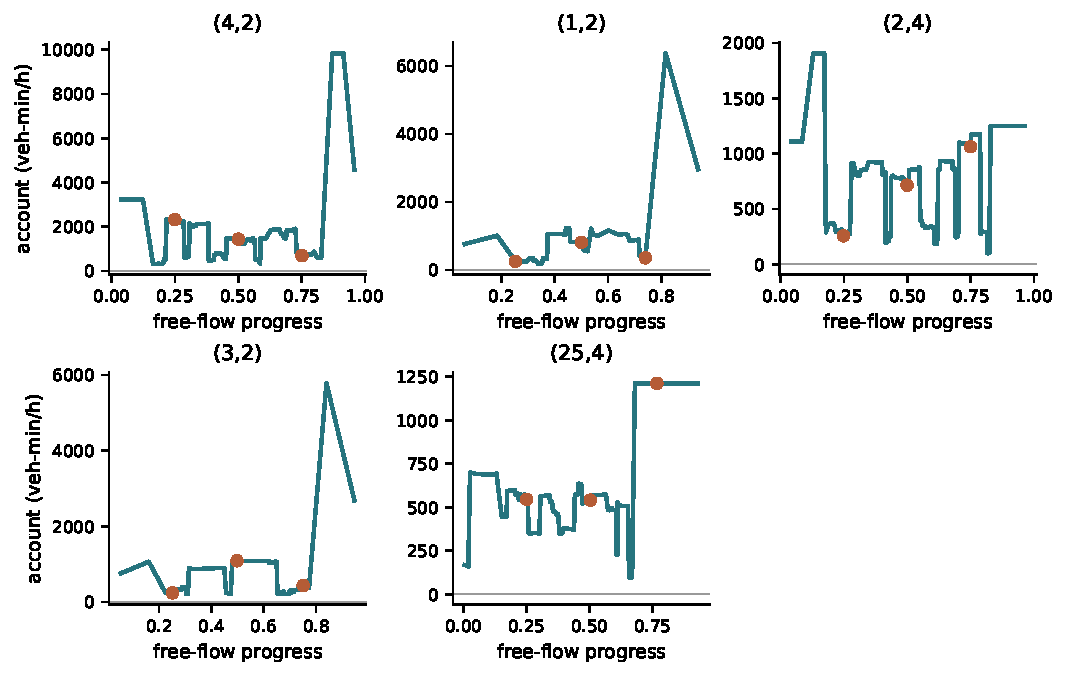
\includegraphics[width=0.99\linewidth]{../figures/fig_v108_anaheim_rest.pdf}
\caption{Anaheim spatial response profiles of the remaining five study
queries over the distance-based families: the account versus free-flow
progress along each query's own OD direction, with ochre dots marking
the three prespecified positions. All stay positive; family ranges span
roughly one to one and a half orders of magnitude.}\label{fig:anaheimrest}
\end{figure}
\begin{table}[pos=htbp]\centering\footnotesize\caption{Anaheim accounts over the complete distance-based family, with the three prespecified positions (vehicle-minutes per hour). Column heads are the prespecified targets; the exact selected levels are (row order) $0.250/0.501/0.752$, $0.252/0.500/0.740$, $0.248/0.499/0.750$, $0.251/0.498/0.751$, $0.251/0.504/0.768$ and $0.250/0.500/0.724$.}\label{tab:anaheim}\begin{tabular}{lrrrrrrr}\toprule OD & System & Unrestricted range & Family range & Regions & $\phi(0.25)$ & $\phi(0.50)$ & $\phi(0.75)$\\\midrule
(4,2) & 34664.1 & [-12712.6,20514.0] & [307.5,9832.1] & 211 & 2323.5 & 1441.8 & 692.3\\
(1,2) & 16773.6 & [-6032.2,9762.0] & [172.7,6374.8] & 83 & 259.0 & 818.0 & 360.5\\
(2,4) & 12143.7 & [-4374.6,6733.0] & [98.7,1905.9] & 211 & 257.0 & 714.6 & 1061.8\\
(3,2) & 14706.7 & [-5613.8,9052.9] & [202.8,5777.4] & 157 & 236.2 & 1087.3 & 434.6\\
(25,4) & 6919.3 & [-1805.3,3091.8] & [96.8,1212.2] & 164 & 545.6 & 540.7 & 1212.2\\
(25,2) & 11445.9 & [-4157.3,6904.5] & [131.8,5751.2] & 84 & 801.5 & 412.0 & 5751.2\\
\bottomrule\end{tabular}\end{table}
\begin{table}[pos=htbp]\centering\footnotesize\caption{Anaheim differences between preselected early and late regions, split by free-flow and congestion weights and study and background responses (vehicle-minutes per hour).}\label{tab:anaheimmechanism}\begin{tabular}{lrrrrr}\toprule OD & Free-flow study & Free-flow background & Congestion study & Congestion background & Total\\\midrule
(4,2) & -416.91 & -8.53 & -1499.94 & 294.16 & -1631.21\\
(1,2) & 9.85 & 6.96 & 83.01 & 1.71 & 101.54\\
(2,4) & 312.07 & -65.41 & 667.06 & -108.90 & 804.83\\
(3,2) & 50.04 & 11.80 & 136.55 & 0.04 & 198.43\\
(25,4) & 47.28 & -40.11 & 666.28 & -6.89 & 666.56\\
(25,2) & -131.77 & -10.52 & 5102.23 & -10.15 & 4949.79\\
\bottomrule\end{tabular}\end{table}

\subsection{Learning objectives and exact endpoint targets}\label{app:learning-objectives}
Equation~\eqref{eq:localboundarybound} suggests learning the reference's weighted demand response
where it affects spatial accounts. With training-only positive scales
$a_j$, the boundary term is
\begin{equation}
\mathcal L=\mathcal L_{\mathrm{flow}}+\lambda_J\mathcal L_{\mathrm{response}}
+\lambda_{\mathrm{cut}}\mathcal L_{\mathrm{boundary}},\qquad
\mathcal L_{\mathrm{boundary}}
=\frac1{NK}\sum_{q,j}\left[\frac{\mathcal K_j(h_j(q))}{a_j}\right]^2.
\label{eq:trainingobjective}
\end{equation}
The reference Jacobian is obtained from the existing implicit SUE
sensitivity system (Appendix~\ref{supp:sue}). We compare ordinary
flow supervision, flow plus response supervision, and the full objective.
Derivative supervision itself is established in Sobolev training
\citep{czarnecki2017sobolev}, including finite-difference derivative targets
\citep{yuan2022sobolev}; the network-derived target here selects the
part of weighted response error that changes boundary accounts.
A circulation in $\ker B$ is invisible to $\mathcal K_j$, so flow and
response losses remain necessary for the other attribution objectives.
The target matches the reference's actual response; it does not force
its true internal attribution divergence to zero or replace TSTT weights
with uniform weights. Equation~\eqref{eq:localboundarybound} is a path
inequality; finite training-point losses alone do not certify an entire
demand domain.


For the following finite-change statement, the outcome is explicitly separable:
\[
g(F)=(g_e(F_e))_{e\in E},\qquad T(F)=\sum_{e\in E}g_e(F_e).
\]
\begin{proposition}[exact finite-change boundary target]\label{prop:pairboundary}
Let $f^L,f^S$ and the edgewise outcome $g$ be continuously differentiable
on an open demand domain, and let $q^\pm=q\pm h e_j$ with their entire
segment in that domain. Put
\[
z_j^r=g(f^r(q^+))-g(f^r(q^-)),\qquad r\in\{L,S\}.
\]
For the attribution of this single-OD change,
\begin{equation}
\max_{U:s_j\in U,\ t_j\notin U}|\phi_j^L(U)-\phi_j^S(U)|
=\mathcal K_j(z_j^L-z_j^S).\label{eq:pairboundaryexact}
\end{equation}
If all sufficiently small single-coordinate changes have matching
accounts on every separating boundary at every point of the domain,
then $BD^LJ_j^L=BD^SJ_j^S$ throughout the domain. Integrating yields
matching boundary attribution columns for any joint demand path in that
domain (with the same columnwise path convention).
\end{proposition}
Appendix~\ref{app:pairproof} proves both statements. The first is an
exact finite-change target, whereas the pointwise response objective
optimizes the upper bound in Eq.~\eqref{eq:localboundarybound}; integrating
before taking $\mathcal K_j$ can retain cancellations. The second statement
requires a domain-wide local premise and is not a guarantee from finite
training data. With several ODs changing, the endpoint outcome difference
only identifies the sum of their attribution columns.

For sampled single-OD endpoint pairs, a direct training objective is
\begin{equation}
\mathcal L_{\mathrm{pair}}=\mathcal L_{\mathrm{flow}}
+\lambda_{\mathrm{edge}}\frac1N\sum_{(q,h,j)}
\frac{\|z_j^L-z_j^S\|_2^2}{b_j^2}
+\lambda_{\mathrm{cut}}\frac1N\sum_{(q,h,j)}
\left[\frac{\mathcal K_j(z_j^L-z_j^S)}{a_j}\right]^2,
\label{eq:pairobjective}
\end{equation}
with positive training-only scales $a_j,b_j$. The edge term controls
changes invisible to the boundary seminorm, whose kernel is $\ker B$.
Two reference endpoint equilibria supply $z_j^S$; training uses ordinary
parameter backpropagation through two predictions, without reference
Jacobian labels or input-Jacobian differentiation. Actual label-generation
and training costs must still be measured.

\subsection{Learned-model evaluation protocol}\label{app:pairs-v102}
Four objectives continue each of five common conservative models for 1,200 Adam
updates, with learning rate $3\times10^{-5}$, flow batch 32 and query batch eight.
The flow data and seed-specific minibatch sequences are shared. Each of six
queries has 64 training and 16 validation endpoint pairs. Centers are sampled
coordinatewise from $[0.65,1.3]$ times baseline demand (seed 102111);
half-widths 2.5\% and 15\% occur equally often. Only one demand changes per
pair, while background routes remain responsive. Endpoint-edge and
endpoint-edge-plus-boundary objectives use identical endpoint labels, coefficients
one and 0.01, and training-only root-mean-square scales. Response supervision
uses derivatives at the same pair centers; its coefficient is one.

The flow loss averages $[(f_e^L-F_e^S)/s_e]^2$ over minibatch states and edges, with $s_e=0.01\sqrt{\operatorname{mean}_{\rm train}[(F_e^S)^2]}$ from the 2,500 training states. The response loss is the batch mean of $\|J_j^L-J_j^S\|_2^2/u_j^2$. With $\langle\cdot\rangle_j$ denoting the average over query $j$'s training pair centers or endpoint labels, the scales are
\[
\begin{aligned}
u_j&=\max\{\sqrt{\langle\|J_j^S\|_2^2\rangle_j},10^{-6}\},\\
b_j&=\max\{\sqrt{\langle\|z_j^S\|_2^2\rangle_j},10^{-6}\},\qquad
a_j=\max\{\sqrt{\langle\mathcal K_j(z_j^S)^2\rangle_j},10^{-6}\}.
\end{aligned}
\]
Edge and response losses sum squared errors over edges before batch averaging; their coefficients are one, while the boundary coefficient is 0.01.

Candidates comprise the common initial model (update zero) and every 100th
continuation update. We minimize normalized validation boundary mean-square
error among candidates with mean endpoint flow error at most 1.1 times the
initial model's value, using the same 96 validation pairs for every method.
The initial model ensures this set is nonempty. Test paths never enter selection.

The final evaluation uses 96 fixed test paths: the 24 paths above
(seed 102112) plus 72 additional paths (seed 102113, 18 per active-query
group) generated by the identical rule; models and validation choices
were frozen before evaluation on the additional paths. Changes
are 15--30\% of baseline demand with both same-direction and mixed-direction
paths, each with 41 states. For every path, flow error first averages relative
Euclidean errors across its states. Attribution statistics average active
queries and seeds within each path and then take medians across the 96 paths;
seeds do not add independent paths. For column error $e_j$ and reference column
$c_j$, relative column, system and unrestricted-boundary errors divide
$\|e_j\|_2$, $|\mathbf1^\top e_j|$ and $\mathcal K_j(e_j)$ by the
corresponding reference values, with absolute floor $10^{-6}$. Geometric error
uses $\max_{U\in\mathcal F_j^{\rm geo}}|\mathbf1_U^\top Be_j|$ and
the same maximum for $c_j$. Percentages multiply ratios by 100.

The decomposition in Eq.~\eqref{eq:coldecomp} is evaluated at the same 41 states
with the same quadrature. Component norms describe error mechanisms; cancellation
prevents treating their norms as additive shares. The fixed-screenline sign
comparison in Appendix~\ref{supp:screenlinelearned} uses the separate frozen
six-query baseline segment and is not pooled with these 24 paths.
\begin{table}[t]\centering\footnotesize
\caption{Four objectives with update zero included in validation selection, on the initial 24-path subset (seed 102112) of the 96-path final evaluation; the full 96-path, five-seed comparison is Table~\ref{tab:pathtable} and the unified four-method comparison is Table~\ref{tab:fourmethods}. All entries report path medians after averaging seeds and active queries.}
\label{tab:pairs-v102}
\begin{tabular}{lrrrrr}\toprule Method & Flow (\%) & Column (\%) & System (\%) & Boundary (\%) & Geometric (\%)\\\midrule
Flow & 0.0325 & 21.61 & 2.33 & 14.53 & 7.91\\
Flow + endpoint edge & 0.0376 & 21.80 & 2.92 & 18.91 & 8.30\\
Flow + endpoint edge + boundary & 0.0376 & 21.81 & 2.95 & 18.93 & 8.30\\
Flow + response & 0.0291 & 14.22 & 3.31 & 12.08 & 5.81\\
\bottomrule\end{tabular}\end{table}
Selected updates in seed order 0--4 are Flow: 1100, 800, 1000, 100, 700; Flow + endpoint edge: 0, 1200, 0, 0, 1100; Flow + endpoint edge + boundary: 0, 1200, 0, 0, 1100; Flow + response: 1100, 1200, 1200, 1200, 1200. All selected models meet the endpoint flow constraint. For each endpoint objective, three seeds retain update zero.
On the original held-out demand-state split, seed-mean relative flow errors are Flow: 0.0386\%, Flow + endpoint edge: 0.0445\%, Flow + endpoint edge + boundary: 0.0445\%, Flow + response: 0.0388\%. These are distinct from the matched-path flow errors in the table.

Table~\ref{tab:learning-costs} reports the incremental computation
costs of training-label generation, common validation and explanation
timing under the shared CPU protocol.
\begin{table}[t]\centering\footnotesize
\caption{Incremental computation costs (seconds). Training-label and common-validation costs are measured separately on the same CPU protocol; training times are archived continuation medians, and explanation times are newly measured sequential medians for the selected models.}
\label{tab:learning-costs}
\begin{tabular}{lrrrr}\toprule Method & Training labels & Common validation & Continuation & Explanation\\\midrule
Flow & 0.00 & 6.45 & 246.0 & 7.34\\
Flow + endpoint edge & 25.75 & 6.45 & 422.2 & 7.59\\
Flow + endpoint edge + boundary & 25.75 & 6.45 & 275.1 & 7.27\\
Flow + response & 16.12 & 6.45 & 297.1 & 7.13\\
\bottomrule\end{tabular}\end{table}
Training labels comprise 768 endpoint states for either endpoint objective, or 384 center states and their sensitivities for response supervision. Every method additionally uses the same 192 endpoint states for validation; unused center-validation derivatives are excluded. Endpoint objectives share their labels and do not incur duplicate reference solves. Existing flow data, pretrained models and the common test reference are excluded from these incremental costs. The 984 test states and sensitivities took 74.4\,s in the archived reference run. Explanation timing covers all 24 paths, forward evaluation, six directional derivatives per state, quadrature and node aggregation, excluding model loading. Archived continuation times include initialization, validation and saving under concurrent seed jobs; they describe the actual training expense and do not establish a method speed advantage.


Across the five selected seeds, the ranges of mean unrestricted-boundary errors are $[13.36,24.12]\%$, $[12.29,30.50]\%$, $[12.27,30.50]\%$, $[10.53,17.46]\%$, respectively, in the method order of Table~\ref{tab:pairs-v102}. Each seed statistic first averages active queries within each path and then gives equal weight to the 24 paths. These ranges describe seed variability rather than additional independent test paths.


\section{Numerical accuracy and supporting results}\label{supp:numdetail}\label{supp:transrecords}
\subsection{Grid refinement, derivative, and solver checks}\label{supp:accuracy}
All differences here are observed numerical comparisons, not certified
bounds. Direct attribution-column differences are at most 0.178\% for
11 versus 41 states and $1.1\times10^{-4}\%$ for six-query/single-OD
41 versus 81 states. Near-zero accounts on 41/81/161 grids change by
less than $5\times10^{-6}$ percentage points (absolute $<0.01$); the
learned 201/801-state relative difference is $4.97\times10^{-6}$.
Implicit versus re-solved central-difference Jacobian errors are at most
$7.6\times10^{-5}$ (halved step $2.5\times10^{-5}$), or
$3.0\times10^{-8}$ for six-query/single-OD columns. Newton versus
successive-averages differences over 1,353 solves are at most
$1.31\times10^{-11}$. Maximum fixed-point and balance residuals are
$3.10\times10^{-8}$ and $1.82\times10^{-11}$ veh/h. Scalar completeness
relative discrepancies are at most $3.36\times10^{-5}$ for
frozen/re-routing settings and $1.9\times10^{-7}$ for single-OD checks.
Per-edge endpoint checks give relative column errors
$7.7\times10^{-8}$--$1.1\times10^{-6}$ and maximum entry residuals
$5.4\times10^{-4}$--$1.6\times10^{-2}$ TSTT units. Per-query records
remain in the arrays. The direct $(10,16)$ account change is 24.80\%
on its 41-state grid; Figure~\ref{fig:respfield} uses the seed-zero
learned model on 201 states (24.8\%).

\subsection{Normalization, cancellation, and sensitivity}\label{supp:additional}
\paragraph{Complete cut-range table.}
Table~\ref{tab:cutspreadfull} completes the three representative rows of
Table~\ref{tab:cutspreadperod} with all eight study ODs.
\begin{table}[pos=htbp]
\footnotesize
\caption{TSTT cut ranges as percentages of each account's absolute
origin-cut value, all eight study ODs (complete version of
Table~\ref{tab:cutspreadperod}). A: zero background; B: frozen background
flows; C: background demands fixed, all traffic re-equilibrated. Learned
values are five-seed medians (ranges); all SUE columns are direct
($41$ quadrature points, implicit sensitivities).}\label{tab:cutspreadfull}
\footnotesize
\begin{tabular*}{\tblwidth}{@{\extracolsep{\fill}}lccccc}
\toprule
& \multicolumn{4}{c}{Unrestricted range (\%)} & Connected (\%)\\
\cmidrule(lr){2-5}\cmidrule(lr){6-6}
OD & Learned A & SUE A & SUE B & SUE C & SUE C\\
\midrule
$(17,10)$ & $59.71$ $(58.92$--$61.23)$ & $59.95$ & $56.38$ & $54.77$ & $35.27$ \\
$(10,17)$ & $37.55$ $(37.40$--$37.94)$ & $37.48$ & $43.62$ & $49.11$ & $31.57$ \\
$(16,10)$ & $36.80$ $(36.41$--$38.40)$ & $36.86$ & $39.99$ & $166.26$ & $127.72$ \\
$(10,16)$ & $26.85$ $(26.68$--$27.07)$ & $26.94$ & $34.02$ & $109.04$ & $83.80$ \\
$(15,10)$ & $0.84$ $(0.69$--$1.16)$ & $0.77$ & $21.98$ & $84.05$ & $58.24$ \\
$(10,15)$ & $0.81$ $(0.76$--$0.88)$ & $0.77$ & $18.89$ & $71.88$ & $49.90$ \\
$(10,11)$ & $0.23$ $(0.10$--$0.35)$ & $0.0075$ & $1.17$ & $84.67$ & $51.27$ \\
$(11,10)$ & $0.18$ $(0.03$--$0.27)$ & $0.0073$ & $0.79$ & $81.09$ & $48.98$ \\
\bottomrule
\end{tabular*}
\end{table}
\paragraph{Error-metric definitions.}
The surrogate test flow error is, within each seed, the mean over the
$857$ test demands of
$\|f(q)-F^{\mathrm{SUE}}(q)\|_2/\|F^{\mathrm{SUE}}(q)\|_2$, reported
as the median over the five seeds; Jacobian column errors
$\|J_j^{\mathrm{learned}}-J_j^{\mathrm{SUE}}\|_2/\|J_j^{\mathrm{SUE}}\|_2$
are pooled over the $5\times41\times8$ seed--point--OD columns;
attribution-column errors use the per-column norm over the $40$
seed--OD columns on the common $41$-point grid.

\paragraph{Same-path flow, sensitivity, and boundary-account errors.}
The test-split flow error is not paired with the Jacobian
comparison; re-summarized on the same $41$ zero-background quadrature
points for each seed (median / 95th percentile / maximum, percent):
flow error $0.136$ / $0.682$ / $1.331$; Jacobian column error
$0.516$ / $3.903$ / $9.562$ (maximum at seed $3$, OD $(16,10)$,
$\lambda=0.925$; $5\times41\times8$ seed--point--OD units);
attribution-column
errors median $0.349\%$, maximum $1.80\%$; and
$E_j^{\mathrm{cut}}$, which evaluates both models' accounts at every
connected boundary of a query's family on the same path
(the unrestricted-family counterpart is virtually identical), at
$0.204$ / $0.650$ / $1.739$ ($40$ seed--OD units; largest connected
error at OD $(16,10)$, seed $3$).

Table~\ref{tab:origin_denominators} supplies the per-query absolute
origin-cut denominators for Table~\ref{tab:cutspreadperod}. The
setting-C link sums $C_j$ span $2.078$--$4.282\times10^5$ TSTT units,
exceeding origin-cut accounts by factors of $1.01$--$2.37$; their sum
matches the endpoint TSTT change within $2.3\times10^{-5}$ relative.
\begin{table}[pos=htbp]
\footnotesize
\caption{Absolute direct-SUE origin-cut accounts
$|\phi_j(\{s_j\})|$, in TSTT units, for the eight queries in
Table~\ref{tab:cutspreadperod}. A, B, C use their respective
$41$-point columns; entries rounded to one decimal.}
\label{tab:origin_denominators}
\footnotesize
\begin{tabular*}{\tblwidth}{@{\extracolsep{\fill}}lrrr}
\toprule
OD & A & B & C\\
\midrule
$(17,10)$ & $29{,}372.1$ & $249{,}729.2$ & $224{,}954.3$ \\
$(10,17)$ & $46{,}977.2$ & $317{,}861.9$ & $245{,}178.7$ \\
$(16,10)$ & $41{,}994.3$ & $352{,}858.5$ & $180{,}671.5$ \\
$(10,16)$ & $57{,}468.9$ & $405{,}374.2$ & $272{,}743.2$ \\
$(15,10)$ & $33{,}859.4$ & $226{,}878.2$ & $201{,}351.2$ \\
$(10,15)$ & $34{,}056.4$ & $258{,}682.3$ & $232{,}160.6$ \\
$(10,11)$ & $28{,}807.1$ & $339{,}651.4$ & $202{,}928.2$ \\
$(11,10)$ & $28{,}010.4$ & $324{,}427.0$ & $204{,}802.3$ \\
\bottomrule
\end{tabular*}
\end{table}

The node breakdown in Table~\ref{tab:bgdecomp} complements the fixed
boundary comparison of Section~\ref{subsec:bgsplit}.
\begin{table}[pos=htbp]
\footnotesize
\caption{Signed node divergence in the re-routing setting, at the
same joint equilibrium state and total-flow gradient at each of the
$41$ quadrature points (study includes all eight query ODs; TSTT
units of Appendix~\ref{supp:networks}; entries rounded independently,
so a component sum may differ from the rounded total in its last
digit).}
\label{tab:bgdecomp}
\small
\begin{tabular*}{\tblwidth}{@{\extracolsep{\fill}}llrrr}
\toprule
OD & Node & Study & Background & Total\\
\midrule
$(10,16)$ & $15$ & $-973.1$ & $49,103.4$ & $48,130.3$ \\
$(10,16)$ & $8$ & $9.6$ & $42,102.7$ & $42,112.3$ \\
$(10,16)$ & $20$ & $0.2$ & $41,805.4$ & $41,805.6$ \\
$(10,11)$ & $5$ & $0.5$ & $35,952.1$ & $35,952.6$ \\
$(10,11)$ & $12$ & $0.0$ & $-23,858.1$ & $-23,858.1$ \\
$(10,11)$ & $9$ & $-0.2$ & $-18,557.6$ & $-18,557.7$ \\
\bottomrule
\end{tabular*}
\end{table}

For the learned zero-background low-range group, five-seed median pointwise
imbalance budgets $100A_j/|\phi_j(\{s_j\})|$ lie between $0.22\%$ and
$0.95\%$, versus $26.85$--$59.71\%$ for the high group; the low-group
median cancellation factors are at most $0.313$ (one seed reaches
$\kappa=0.852$), so small pointwise imbalance mainly limits the
low-group range, while the high group's median $\kappa$ is below
$8\times10^{-5}$.

Zero-background route-choice dispersion checks at $\theta\in\{0.5,1,2\}$
(eleven-point direct-SUE calculations) retain the large/small
separation --- large ranges $27$--$64\%$, the others below $9.4\%$.

\subsection{Full-background six-query surrogate validation}\label{supp:fullbgsurrogate}
The six-query conservative surrogate predicts shares over all 5,280
paths, with the architecture of Appendix~\ref{supp:protocol}, dataset
seed 20261025 and batch size 256. Its 4,214 target solves have maximum
path residual $3.5\times10^{-8}$; learned conservation residual is at
most $3.6\times10^{-11}$. Held-out flow error is 0.040\% (seed median;
range 0.035--0.056\%). On the 41 common path states, flow errors are
0.037--0.065\%, but increment errors are 5.0--7.0\% against a reference
increment norm 2,982.7 (2.7\% of flow level). Median column errors are
81.2\% for $(7,18)$, 31.1\% for $(4,5)$ and 7.4--11.8\% for the
others. System contribution errors reach 14.7\% and 10.3\% for those
two queries, versus at most 3.7\% for the sign-crossing queries.
Learned column completeness is within $6\times10^{-6}$ relative;
across-seed envelopes of the learned columns and connected extrema
accompany the result arrays.

An exact two-term split of \eqref{eq:Cdef} ($L$/$S$: learned/direct)
identifies where this error arises:
\begin{equation}
\widetilde C_{:,j}^{L}-\widetilde C_{:,j}^{S}
=\Delta q_j\int_0^1(D_\lambda^{L}-D_\lambda^{S})J_j^{S}\,\mathrm{d}\lambda
+\Delta q_j\int_0^1D_\lambda^{L}(J_j^{L}-J_j^{S})\,\mathrm{d}\lambda,
\label{eq:coldecomp}
\end{equation}
satisfied entrywise within $10^{-10}$ TSTT units. The weight-shift
term has querywise median norm at most 0.2\% of the reference column;
the response term is larger in every one of the thirty seed--query
units. Their norm sum is at most 1.04 times the realized error norm.
Signed scalar terms can cancel, so these norms are not additive shares.
Small-band endpoint columns have 4.8--15.9\% error and system values
within 2.7\% of reference, while every seed retains the reported signs.

\subsection{Sensitivity to candidate paths and route-choice dispersion}\label{supp:coverage}
The path-set comparison expands all $528$ OD sets to twenty
candidates each (the first ten unchanged), with demands, BPR
functions, $\theta=1$, and $41$ quadrature points fixed: across the
eight queries, absolute unrestricted and connected ranges change by
at most $0.977\%$ and $1.011\%$, with the three largest
internal-node terms keeping their ordered node IDs (moving at most
$1.43\%$). The $\theta\in\{0.5,2\}$ check splits the specified
$(10,16)$ boundary difference into study/background components
$-7{,}404.9$/$-2{,}371.5$ at $\theta=0.5$ and $+115.3$/$+235.7$ at
$\theta=2$; for all three additional models, implicit derivative
columns match re-solved half-step central differences at the
demand-path midpoint (maximum $0.00249\%$, completeness gap
$2.85\times10^{-5}$).

\subsection{Six-query interval, mechanism, boundary-family, and
scenario checks}\label{supp:newodaccuracy}


\textbf{Extremal ranges and negative shares.}
Unrestricted extrema follow the closed form \eqref{eq:cutextrema},
connected extrema the same enumeration as the connected ranges
(Table~\ref{tab:newodinterval}); the negative shares in
Section~\ref{subsec:newod} are exact counts over the connected
families ($4{,}621$--$16{,}943$ admissible sets per query), and all
displayed values come from the $41$-point columns.

\begin{table}[pos=tbh]
\footnotesize
\caption{Minimum--maximum boundary-account ranges for the three
sign-crossing queries of Table~\ref{tab:newod}, in TSTT units
(Appendix~\ref{supp:networks}), rounded to integers. Baseline:
unrestricted extrema (closed form \eqref{eq:cutextrema}; connected
extrema in Table~\ref{tab:newod}); next four rows: connected
ranges under the model-setting changes and the single-OD
$0.2\to1.6$ re-run (unrestricted intervals within $1\%$ of the
baseline row); last two: small-interval bands, with $C_j$ positive
($+7{,}202$ to $+33{,}734$ across the three queries) and the control
$(6,8)$ positive ($[5{,}079,\ 9{,}623]$ and $[10{,}157,\ 19{,}246]$;
single-OD $[35{,}352,\ 66{,}861]$).}
\label{tab:newodinterval}
\footnotesize
\begin{tabular*}{\tblwidth}{@{\extracolsep{\fill}}lrrr}
\toprule
Range & $(1,19)$ & $(1,15)$ & $(7,12)$\\
\midrule
Baseline ($10$ paths, $\theta=1$): unrestricted & $[-19{,}116,\ 26{,}696]$ & $[-16{,}240,\ 44{,}137]$ & $[-45{,}241,\ 61{,}650]$\\
\addlinespace
Twenty paths, $\theta=1$: connected & $[-13{,}451,\ 24{,}276]$ & $[-8{,}329,\ 40{,}644]$ & $[-17{,}728,\ 59{,}452]$\\
Ten paths, $\theta=0.5$: connected & $[-13{,}024,\ 24{,}064]$ & $[-8{,}107,\ 39{,}933]$ & $[-17{,}633,\ 60{,}476]$\\
Ten paths, $\theta=2$: connected & $[-13{,}016,\ 24{,}411]$ & $[-8{,}233,\ 40{,}892]$ & $[-19{,}587,\ 61{,}647]$\\
Single-OD $0.2\to1.6$: connected & $[-13{,}608,\ 24{,}414]$ & $[-8{,}359,\ 40{,}745]$ & $[-17{,}580,\ 60{,}006]$\\
Single-OD $\pm10\%$ band ($0.9\to1.1$): connected & $[-1{,}947,\ 3{,}494]$ & $[-1{,}201,\ 5{,}838]$ & $[-2{,}517,\ 8{,}608]$\\
Single-OD $\pm20\%$ band ($0.8\to1.2$): connected & $[-3{,}895,\ 6{,}988]$ & $[-2{,}402,\ 11{,}677]$ & $[-5{,}035,\ 17{,}215]$\\
\bottomrule
\end{tabular*}
\end{table}

\textbf{Connected minimum and divergence decomposition.}
Table~\ref{tab:negmech} reports, for each sign-crossing query, the
connected minimizing boundary $U_-$ at the baseline setting: its
account, and the interior divergence sum
$\phi_j(\{s_j\})-\phi_j(U_-)$, decomposed as the table caption
specifies, at the same joint state and gradient as the reported
columns (additivity $\le1.2\times10^{-10}$).
By Eq.~\eqref{eq:cutgap}, the negative divergence captured inside
$U_-$ ($4{,}664.9$, $6{,}960.1$, and $19{,}811.5$ for the three
queries) covers $83\%$, $88\%$, and $72\%$ of the gaps
$\phi_j(U_-)-\phi_j^{\min}$, while the captured positive divergence
($19{,}938.0$, $18{,}194.2$, $46{,}901.4$) is $95.5\%$, $94.8\%$,
and $85.7\%$ of the query totals. The sign change arises
differently across queries: study response
dominates for $(1,19)$ (largest node $15$: own $+14{,}464.0$),
study- and background-dominated nodes share the sign for $(1,15)$,
and both contribute about equally for $(7,12)$ (node $8$).
The extremal node sets (one-based node IDs) are
$U_-(1,19)=\{1,2,6,7,8,9,15,16,18,20,21,22,24\}$ and
$U_+(1,19)=\{1,2,3,4,5,6,10,11,12,13,14,22,23\}$;
$U_-(1,15)=\{1,2,6,7,8,9,16,17,18,19,20,21,24\}$ and
$U_+(1,15)=\{1,2,3,4,5,6,10,11,12,13,14,22,23\}$;
$U_-(7,12)=\{1,2,3,4,5,6,7,8,9,10,11,14,17,19,23\}$ and
$U_+(7,12)=\{7,8,9,15,16,18,20,21,22,24\}$.

\begin{table}[pos=tbh]
\footnotesize
\caption{Connected minimizing boundary $U_-$ at the baseline setting
for the three sign-crossing queries, in TSTT units. Interior is the
divergence sum over $U_-\setminus\{s_j\}$, decomposed into the query's
own response, the other five query ODs, and the background response;
the study group of the main text is the sum of the first two columns.
Node sets are the one-based lists in the preceding paragraph. Entries
are rounded independently.}
\label{tab:negmech}
\small
\begin{tabular*}{\tblwidth}{@{\extracolsep{\fill}}lrrrrrr}
\toprule
OD & $\phi_j(\{s_j\})$ & $\phi_j(U_-)$ & Interior & Own OD & Other query & Background\\
\midrule
$(1,19)$ & $1{,}771.6$ & $-13{,}501.6$ & $15{,}273.1$ & $19{,}480.9$ & $-59.4$ & $-4{,}148.3$ \\
$(1,15)$ & $2{,}948.1$ & $-8{,}286.0$ & $11{,}234.1$ & $7{,}856.9$ & $-26.7$ & $3{,}404.0$ \\
$(7,12)$ & $9{,}473.8$ & $-17{,}616.2$ & $27{,}089.9$ & $14{,}002.3$ & $-3.2$ & $13{,}090.8$ \\
\bottomrule
\end{tabular*}
\end{table}

\textbf{Neighbourhood families.}
Use undirected hop distance or shortest free-flow distance from the origin
(minimum weight over parallel arcs). Include nodes at each attained radius,
stop before including the destination, and retain only two-sided connected
regions. Table~\ref{tab:neighbourhoods} reports all family ranges; all are
positive with minima at the origin cut. For short-path queries $(7,18)$,
$(4,5)$ and $(6,8)$, only that cut is admissible. The thirteen-node
free-flow ball at radius 16 for $(1,19)$ is
$\{1,2,3,4,5,6,7,8,9,11,12,13,24\}$, with account $+10{,}756.0$.

\begin{table}[pos=htbp]
\footnotesize
\caption{Origin-centred neighbourhood accounts, baseline six-query setting C
(TSTT units). Counts are distinct admissible node sets within each family;
sets shared by the two families are counted in each row.}\label{tab:neighbourhoods}
\footnotesize
\begin{tabular*}{\tblwidth}{@{\extracolsep{\fill}}llrrr}
\toprule OD & Neighbourhood & Count & Minimum & Maximum\\\midrule
$(1,19)$ & Hop distance & 6 & $1,771.6$ & $15,803.5$\\
$(1,19)$ & Free-flow time & 13 & $1,771.6$ & $15,803.5$\\
$(1,15)$ & Hop distance & 5 & $2,948.1$ & $26,602.0$\\
$(1,15)$ & Free-flow time & 14 & $2,948.1$ & $26,602.0$\\
$(7,12)$ & Hop distance & 4 & $9,473.8$ & $31,524.1$\\
$(7,12)$ & Free-flow time & 9 & $9,473.8$ & $32,139.4$\\
\bottomrule\end{tabular*}\end{table}

\textbf{Straight screenlines.}
Coordinates use an equirectangular frame (longitude scaled by the cosine
of mean latitude). Section~\ref{sec:scan}'s 36-direction construction,
with duplicate regions removed, gives 35, 152, 32, 123, 23 and 148
regions in Table~\ref{tab:newod} order. All accounts agree with direct
incidence aggregation below $10^{-9}$. Refining directions from
$5^\circ$ to $1^\circ$ leaves both negative minima unchanged; negative
shares change from 1.3\% to 1.8\% for $(1,19)$ and 6.8\% to 6.2\%
for $(7,12)$. Other queries stay positive; only $(7,18)$'s minimum
changes, from 642.4 to 641.4.

\textbf{Model-setting checks.}
Re-solving the protocol of Appendix~\ref{supp:newod} under twenty
candidate paths per OD and $\theta\in\{0.5,2\}$ at ten paths gives
the ranges of Table~\ref{tab:newodinterval} ($C_j$ within $3.9\%$);
solver and finite-difference checks match
Appendix~\ref{supp:newod} levels.

\textbf{Single-OD demand changes.}
Each single-OD demand path ($0.2\to1.6$ of published demand)
re-solves the setting-C protocol with one moving coordinate. For the
three crossing queries the connected ranges (Table~\ref{tab:newodinterval},
single-OD row) still straddle zero, their extrema attained by exactly
the joint-scenario sets $U_-$ and $U_+$ (changes at most $0.9\%$ and
$0.5\%$; unrestricted intervals within $1\%$ of the joint baseline)
and the contributions stay positive ($C_j=50{,}322.2$, $77{,}672.6$,
$117{,}476.8$); the control $(6,8)$ remains sign-consistent
($C_j=74{,}176.1$, connected range in the caption). The
small-interval bands (Table~\ref{tab:newodinterval}, last two rows)
follow the same protocol, the $41$-point check ($(1,19)$,
$0.8\to1.2$) reproducing the endpoint column to $1.3\times10^{-5}$
TSTT units per edge.

\begin{figure}[pos=htbp]
\centering
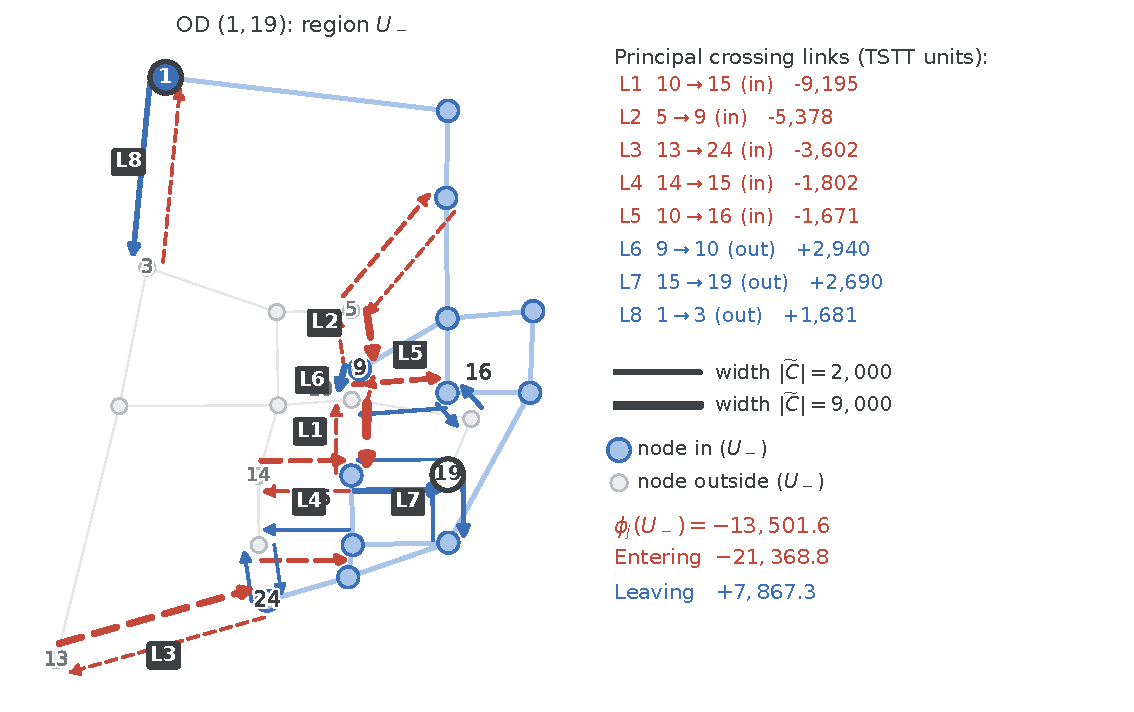
\includegraphics[width=0.82\linewidth]{../figures/fig_negmech_v102.pdf}
\caption{The connected minimizing region $U_-$ for OD $(1,19)$
(setting C, six-query protocol). Shaded nodes form $U_-$ (origin
node $1$ ringed; destination $19$ outside). Crossing-link arrows keep
the link direction; width scales with $|\widetilde C_{e,j}|$, and
colour and style encode the signed contribution to $\phi_j(U_-)$,
$a_{e,j}=\sigma_e\widetilde C_{e,j}$ ($\sigma_e=+1$ leaving, $-1$
entering; solid blue positive, dashed red negative), so a positive
attribution on an entering link appears red. The side panel lists, in
TSTT units, the five largest negative and three largest positive
contributions among the $26$ crossing links
($\mathrm{L}1$--$\mathrm{L}5$ negative, $\mathrm{L}6$--$\mathrm{L}8$
positive, ``(in)''/``(out)'' marking entering and leaving links),
with the width scale and the membership legend.}
\label{fig:negmech}
\end{figure}
\textbf{Endpoint identity checks.}
Appendix~\ref{supp:accuracy} reports the per-edge
endpoint-identity errors and their relation to completeness gaps on
these same demand paths.

\FloatBarrier
\subsection{Frozen-surrogate boundary errors}\label{supp:screenlinelearned}
Table~\ref{tab:screenlinelearned} reports, for each of the six study
queries, the reference minimum over the fixed straight screenline
family and the accounts of the five frozen flow-supervised surrogates
at that same screenline, with the across-seed range of the largest
family error in the last column. On the connected families of the same
protocol, the five-seed median largest connected-boundary disagreement
is $4.2$--$6.9\%$ of the direct connected span for four queries,
reaches $99.5\%$ for the small-response query $(4,5)$ and exceeds the
span ($522.5\%$) for $(7,18)$; across-seed envelopes of the learned
columns and connected extrema accompany the result arrays.
\begin{table}[pos=htbp]
\footnotesize
\caption{Fixed straight screenlines: reference minimum and the five frozen flow-supervised surrogates at that same screenline (TSTT units). The last column gives the largest error over the screenline family, as an across-seed range.}
\label{tab:screenlinelearned}
\small\begin{tabular*}{\tblwidth}{@{\extracolsep{\fill}}lrrr}\toprule
OD & Reference minimum & Learned account: seed range & Maximum screenline error: seed range\\\midrule
$(7,18)$ & 642.4 & $[576.9,\ 789.8]$ & $[141.0,\ 269.4]$ \\
$(1,19)$ & -2766.6 & $[-3886.6,\ -3365.1]$ & $[857.9,\ 1430.8]$ \\
$(4,5)$ & 2652.3 & $[2301.7,\ 2918.8]$ & $[438.0,\ 648.3]$ \\
$(1,15)$ & 511.1 & $[732.8,\ 2068.2]$ & $[1140.6,\ 2553.0]$ \\
$(6,8)$ & 45230.2 & $[46431.5,\ 47218.3]$ & $[1276.2,\ 1988.1]$ \\
$(7,12)$ & -2967.3 & $[-2810.4,\ -1916.6]$ & $[1736.8,\ 2499.2]$ \\
\bottomrule\end{tabular*}\end{table}


All five baseline seeds retain the three connected-family sign
crossings and positive system contributions. At the fixed reference
extrema,
$m_j=\min\{-\phi_j^S(U_-),\phi_j^S(U_+)\}-\epsilon_j^{\rm conn}$
is positive, with smallest value 5519 TSTT units. At the fixed
direct-model minimizing screenline, every seed retains the negative
sign for both queries: $(1,19)$ gives $[-3886.6,-3365.1]$ against the
reference $-2766.6$, and $(7,12)$ gives $[-2810.4,-1916.6]$ against
$-2967.3$, with largest family-wide errors $1430.8$ and $2499.2$ below
the reference sign margins. These are screenline-specific certificates
of sign preservation; they do not imply accurate column magnitudes.


The eight-query path-set and dispersion checks are collected in
Appendix~\ref{supp:coverage}. Boundary variation persists, although
the specified $(10,16)$ comparison $\{10\}\to\{10,17\}$ changes sign
across $\theta$; these are different fixed-path models, not convergence
to unrestricted SUE.

\subsection{Additional learning comparisons}\label{app:legacy-learning}\label{app:learning-protocol}\label{app:calibration-protocol}
Two additional pointwise comparisons use five conservative models, 600 Adam updates at $3\times10^{-5}$, flow/response batches of 32/8 and training-only scales. Derivative labels comprise 256 training and 64 validation states (seed 20261029). The fixed-coefficient comparison uses coefficients one; calibration selects 0.01 from $\{0.001,0.01,0.1\}$ with seed zero under a 110\% relative flow-error threshold, then applies it across seeds (seven boundary fits). Each comparison tests four prescribed 41-state paths, with one, two, three and six active queries and baselines in $[0.65,1.3]$ times published demands (test seeds 101029/101030). Fixed-coefficient boundary supervision yields 22.25\% boundary error versus 9.64\% for response supervision; calibration yields 7.74\% versus 7.44\% on its new paths. Neither
comparison supports overall improvement. The final four-method
comparison with common selection and matched-path metrics is
Table~\ref{tab:fourmethods}.

\subsection{Group-level uncertainty for the 96-path comparison}\label{supp:learningdetail}
Path-level bootstrap intervals for the paired median differences
(10,000 resamples; column error / geometric error, in percentage
points): single-query group $[-4.90,-2.95]$ / $[-1.99,-0.88]$
improving 24/24 and 23/24 paths; two-query group $[-6.48,-4.31]$ /
$[-3.15,-1.52]$, 22/24 and 21/24; three-query group $[-9.26,-3.36]$ /
$[-4.11,-1.36]$, 22/24 and 22/24; six-query group $[-8.59,-5.22]$ /
$[-3.86,-1.73]$, 24/24 and 24/24. Leave-one-path-out medians of the
paired column difference vary within $[-5.11,-4.94]$ and of the paired
geometric difference within $[-2.11,-2.00]$, so no single path carries
the result. The system-contribution difference has median $+0.45$
percentage points with interval $[0.01,0.74]$, improving 39 of 96
paths, while both methods retain system errors below $3.5\%$ (medians
$2.52\%$ and $3.13\%$).

\subsection{Unrestricted and integrated-bound errors by group}\label{supp:boundchain}
Table~\ref{tab:boundchain96} completes Table~\ref{tab:pathtable} with
the unrestricted and integrated-bound columns of
Eq.~\eqref{eq:localboundarybound}, as percentages of the reference
column's boundary seminorm; the geometric and unrestricted columns use
different denominators and are not one inequality, and the bound chain
$\mathcal K_j(e_j)\le B_j$ holds in absolute units for the shared
quadrature (Section~\ref{sec:pairresults}).
\begin{table}[pos=htbp]\centering\footnotesize
\caption{Unrestricted (exact $\mathcal K_j(e_j)$ over all separating
regions) and bound (integrated bound of
Eq.~\eqref{eq:localboundarybound}) errors, medians of path-level values
on the 96 test paths, as percentages of the reference column's
boundary seminorm.}\label{tab:boundchain96}
\begin{tabular}{rcc cc}\toprule
& \multicolumn{2}{c}{Unrestricted (\%)} & \multicolumn{2}{c}{Bound (\%)}\\
\cmidrule(lr){2-3}\cmidrule(lr){4-5}
Active & flow & resp. & flow & resp.\\\midrule
1 & 4.54 & 2.95 & 4.62 & 3.00\\
2 & 15.48 & 12.65 & 15.67 & 12.80\\
3 & 16.36 & 12.39 & 16.70 & 12.81\\
6 & 19.43 & 12.28 & 20.61 & 13.48\\
\midrule
All 96 & 15.65 & 12.08 & 16.34 & 12.83\\
\bottomrule\end{tabular}\end{table}

\subsection{Complete input-stratified common-summary results}\label{sec:coverage}
Positive non-diagonal published demands are stratified by demand and directed free-flow shortest-path time using empirical tertiles, with ties kept in the lower bin. Within each of nine cells, lexicographically sorted OD indices at zero-based positions $\lfloor N/3\rfloor$ and $\lfloor2N/3\rfloor$ are retained. No attribution values enter selection. Endpoint differences identify total edge attribution, without identifying the same-state study/background response split. The two perturbation widths share every field of the selection protocol and differ only in the demand interval; their normalized errors are close for every query, so Table~\ref{tab:coveragefull} reports both in one table. Absolute minima, maxima, midpoints and half-ranges for both widths, and the per-position account sequences behind the segmentation of Proposition~\ref{prop:segmented}, accompany the result arrays in the code package. Figure~\ref{fig:coverageintervals} plots the complete interval set, normalized by each query's largest account magnitude; each query's common value and error follow from the tabulated range by the midpoint rule $\beta=(\phi_{\min}+\phi_{\max})/2$.
\begin{table}[pos=htbp]\centering\footnotesize\caption{Complete geometric common summaries for the 18 input-stratified queries at both widths. Normalized error is Eq.~\eqref{eq:normerror} at $\pm10\%$ and $\pm20\%$; ranges are $[\phi_{\min},\phi_{\max}]$ at $\pm20\%$ in Sioux Falls cost units; P and M mean positive and mixed signs at $\pm20\%$.}\label{tab:coveragefull}\begin{tabular}{lrrrrl}\toprule OD & System & Range ($\pm20\%$) & Norm.\ err.\ ($\pm10\%$) & Norm.\ err.\ ($\pm20\%$) & Sign\\\midrule
(4,3) & 507.2 & [429.0, 535.0] & 9.9 & 9.9 & P\\
(12,3) & 337.2 & [330.7, 340.2] & 1.4 & 1.4 & P\\
(6,1) & 2360.6 & [658.3, 2290.4] & 35.6 & 35.6 & P\\
(15,6) & 9390.2 & [415.4, 4433.5] & 45.3 & 45.3 & P\\
(6,21) & 4577.8 & [-3.4, 2349.4] & 50.1 & 50.1 & M\\
(18,14) & 3422.3 & [150.8, 1929.7] & 46.1 & 46.1 & P\\
(8,4) & 25097.5 & [1270.7, 15741.3] & 46.0 & 46.0 & P\\
(19,8) & 16939.7 & [733.2, 7266.4] & 45.0 & 45.0 & P\\
(11,6) & 6165.9 & [1236.4, 6106.4] & 39.9 & 39.9 & P\\
(16,2) & 17763.1 & [896.3, 9628.6] & 45.3 & 45.3 & P\\
(8,21) & 7605.5 & [752.6, 4214.1] & 41.1 & 41.1 & P\\
(14,8) & 17445.3 & [890.3, 7527.1] & 44.1 & 44.1 & P\\
(11,15) & 47925.5 & [17628.9, 27737.8] & 18.2 & 18.2 & P\\
(17,9) & 24040.9 & [5482.3, 18519.3] & 35.2 & 35.2 & P\\
(10,12) & 55214.5 & [9822.4, 33248.6] & 35.2 & 35.2 & P\\
(13,10) & 54411.9 & [2918.8, 31345.2] & 45.3 & 45.3 & P\\
(1,10) & 33917.2 & [2182.9, 20856.4] & 44.8 & 44.8 & P\\
(10,1) & 34264.5 & [2182.7, 21039.5] & 44.8 & 44.8 & P\\
\bottomrule\end{tabular}\end{table}

\begin{figure}[pos=htbp]\centering
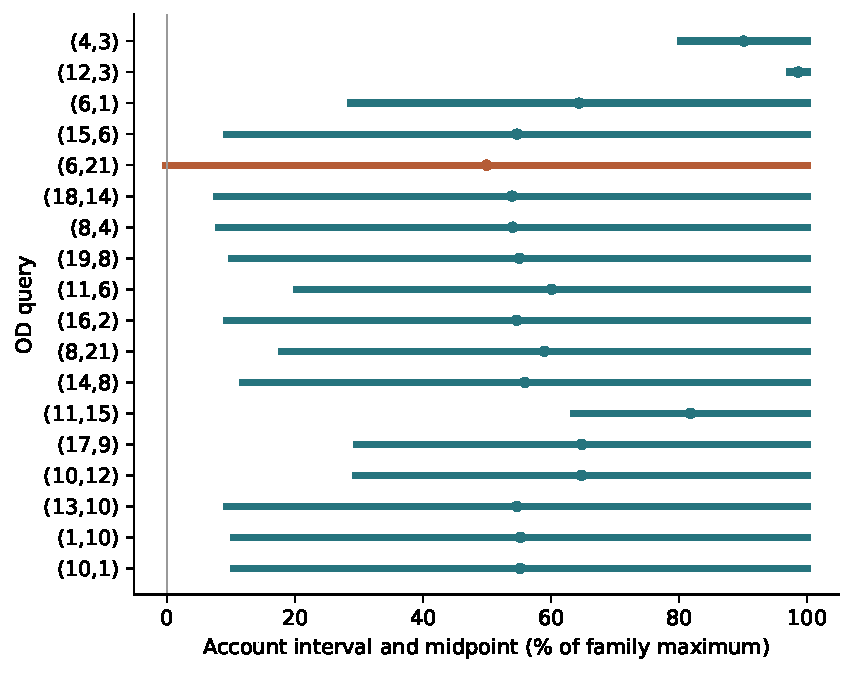
\includegraphics[width=0.88\linewidth]{../figures/fig_v108_coverage_intervals.pdf}
\caption{Geometric account intervals normalized by each query's largest
account magnitude, over all 18 input-stratified queries at $\pm20\%$
(the complete-interval companion of
Figure~\ref{fig:commonsummary}).}\label{fig:coverageintervals}
\end{figure}

\begin{table}[pos=htbp]\centering\footnotesize
\caption{Tolerance sensitivity of the delivered summaries, within
fixed projection directions (experiment C for Sioux Falls, 18 queries
per level, 36 normals with duplicate chains removed; experiment D for
Anaheim, six single-direction queries). Single: number of queries whose
whole family admits one common value at the stated tolerance;
segments: median per-direction count on Sioux Falls at load levels
$0.7/1.0/1.3$ (maximum over directions in parentheses) or per-query
range on Anaheim; compression: $1-$segments/regions, median per
direction (Sioux Falls) or per query (Anaheim).}\label{tab:tolerance}
\begin{tabular}{rrrrr}\toprule
Tolerance $\tau$ & Sioux single ($0.7/1.0/1.3$) & Sioux med.\ seg./dir. & Anaheim segments & Anaheim compression\\\midrule
$2.5\%$ & $2/1/0$ & $4.0\,(10)/4.5\,(12)/5.5\,(13)$ & $6$--$21$ & $91.5\%$\\
$5\%$ & $2/1/0$ & $3.0\,(7)/4.0\,(8)/4.5\,(10)$ & $4$--$14$ & $93.8\%$\\
$7.5\%$ & $2/1/1$ & $2.0\,(7)/3.0\,(8)/3.0\,(8)$ & $3$--$12$ & $95.5\%$\\
$10\%$ & $2/2/1$ & $2.0\,(6)/2.0\,(6)/2.5\,(7)$ & $3$--$12$ & $96.4\%$\\
\bottomrule\end{tabular}\end{table}

\paragraph{Tolerance rule and small-magnitude detail.}\label{supp:tolerance}
The primary rule is absolute: $\epsilon_j=5\%$ of the family's largest
account magnitude, so it permits errors much larger than $5\%$ of the
small accounts. A mixed rule
$|\hat a_i-a_i|\le\epsilon_{\mathrm{abs}}+\tau|a_i|$ keeps relative
control at small magnitudes; a candidate segment admits a common
representative iff $\max_{i\in I}(a_i-t_i)\le\min_{i\in I}(a_i+t_i)$
with $t_i=\epsilon_{\mathrm{abs}}+\tau|a_i|$, feasibility is inherited
by subintervals, and the same greedy returns the minimum count. On
Anaheim, at the primary rule the worst relative error at
small-magnitude positions (accounts below $10\%$ of the family
maximum) has median $0.55$ and maximum $0.94$; the mixed rule with
$\epsilon_{\mathrm{abs}}=1\%$ of the family maximum and $\tau=10\%$
lowers these to $0.28$ and $0.45$ while the median segment count rises
from 10 to 12 (per-query range 6--17), i.e.\ the compression is
essentially retained and the detail at small-magnitude positions
doubles in accuracy. Enlarging the relative part of the primary
$5\%$ absolute rule without shrinking the absolute floor
($\epsilon_{\mathrm{abs}}=5\%$, $\tau\ge5\%$) instead reduces
segment counts by merging large-magnitude runs while the
small-position error worsens --- confirming that the absolute floor,
not the relative part, controls the small-magnitude detail.

\paragraph{Load-level protocol and node-imbalance diagnostics.}
The load-level experiment solves one equilibrium per level ($0.7$,
$1.0$, $1.3$ times the published demands); with the focal query moving
alone over $\pm20\%$ under the identical geometric family and masks,
the levels $0.7$ and $1.3$ add 74 equilibrium solves. For each of the
18 columns and three levels, the imbalance vector $d_j$ of
Eq.~\eqref{eq:endpointd} has norm $\norm{d_j}_2$ rising from a median
of $1196.4$ at level $0.7$ to $4803.2$ at $1.0$ and $15763.3$ at
$1.3$ --- a $13.2$-fold increase from the light to the heavy baseline
--- while the unrestricted range $S_j$ rises from $3102.2$ to
$52766.2$. Across all 54 query--level pairs, the rank correlation
between $\norm{d_j}_2$ and the geometric-family spread is $0.99$
(Spearman; $0.99$ for $S_j$), and the realized ratio
$S_j/\norm{d_j}_2$ has median $2.53$ against the Cauchy--Schwarz bound
$\sqrt{n-2}=4.69$ of Eq.~\eqref{eq:rangebound}. The normalized
summary error, whose denominator varies by query, correlates more
moderately ($0.53$). The load levels change the realized weights,
responses and demand increments together rather than the weights alone,
so these correlations are mechanism-consistent readings of
Eq.~\eqref{eq:cutspread}, not isolated weight effects.

\subsection{Computational protocol for alternative attribution orders}\label{supp:pathrobust}
Each of the 22 alternative orders of Section~\ref{subsec:pathrobust}
changes the six study ODs one at a time (41 quadrature states per
segment, identical solver tolerance, endpoints and boundary family as
the straight-line run; canonical order, reverse order, and twenty
permutations under seed 20261031). Gates: straight-line columns
reproduce the frozen arrays to $1.7\times10^{-15}$ relative; every
order's endpoint equilibria match the straight-line endpoints to
$6.1\times10^{-9}$; the path-independent total outcome change
reproduces to $1.5\times10^{-7}$ relative. Each order's record stores
the attribution column, family range, common summary and normalized
error, sign-crossing flag, maximum profile deviation against the
straight-line accounts, and mechanism components at the fixed regions
$U_-$ (arrays in the code package). The dominant mechanism at $U_-$
coincides with the straight line's on all 22 orders for each of the
three mechanism-tracked queries.

\subsection{Anaheim learned-assignment protocol}\label{app:anaheimlearning}
The Anaheim experiment mirrors the Sioux Falls protocol in structure;
differences are stated here once. The study queries are the six largest
published OD demands of Section~\ref{sec:anaheim}; all remaining
positive demands are fixed with endogenous route choice over the same
ten-path centroid-restricted structure. The model is the conservative
parameterization of Eq.~\eqref{eq:consparam} with $K=1{,}406$ OD
softmaxes over $P=14{,}060$ paths and $m=914$ link outputs; the input
is the six-dimensional study demand vector. Reference labels: 1{,}000
flow states ($q\sim U(0.65,1.3)\,q_{\mathrm{base}}$; 800 train, 200
validation), 480 derivative centers (384 train, 96 validation) with
equilibrium sensitivities of the six study columns, and 48 test demand
paths (twelve per active-query group $k\in\{1,2,3,6\}$, mixed and same
signs, generation rule identical to the Sioux Falls test paths under a
fresh seed) solved at a 21-state quadrature with sensitivities at every
state. Training: stage~A pretrains flow-only from scratch for up to
4{,}000 steps (Adam, learning rate $3\times10^{-3}$, batch 128,
per-link scaled MSE, best-validation selection every 50 steps); stage~B
continues for 1{,}200 steps with the method objective exactly as in
the Sioux Falls protocol (learning rate $3\times10^{-5}$, batch 32
flow samples plus 8 derivative centers, rotation over the six study
columns), methods \emph{flow} and \emph{response}, five seeds.
Validation: flow relative error on the 200 held-out flow states;
$K$-MSE, the boundary-seminorm of the weighted response discrepancy
normalized per query, on the 96 held-out centers. Selection: minimum
validation $K$-MSE among states with validation flow error at most
1.1 times the stage-A checkpoint, fallback minimum flow error; test
paths enter neither training nor selection. All selected response
checkpoints lie at the 1{,}200-step training cap, as in Sioux Falls,
so the operating point is budget-limited rather than
validation-plateaued; the conclusion is nevertheless uniform across
seeds. Gates: conservation of every reference state (study plus
background supply) holds to $9.1\times10^{-12}$ vehicle-units;
reference-column completeness relative to the endpoint outcome change
is at most $1.2\times10^{-5}$; the total error of every delivered
summary stays within its budget. Costs: reference data 2{,}488
equilibrium solves with sensitivities ($\approx$35\,s per state
single-threaded, parallelized over twelve workers), pretraining
$\approx$40\,minutes per seed, fine-tuning $\approx$5--9\,minutes per
(method, seed).


\end{document}
